%%================================================
%% Filename: main.tex
%% Encoding: UTF-8
%% Author: Yuan Xiaoshuai - yxshuai@gmail.com
%% Created: 2012-01-08 13:09
%% Last modified: 2020-04-05 21:01
%%================================================
% !TEX program = xelatex
\documentclass[bachelor]{zzuthesis}
% \documentclass[%
%   bachelor|master|doctor% mandatory option
%   ]{zzuthesis}
% 自定义宏包
\usepackage{docutils}

% 图形文件路径
\graphicspath{{figures/}}

\begin{document}
\frontmatter
%%================================================
%% Filename: cover.tex
%% Encoding: UTF-8
%% Author: Yuan Xiaoshuai - yxshuai@gmail.com
%% Created: 2012-01-14 13:44
%% Last modified: 2019-11-03 00:30
%%================================================
% 研究生论文:学校代码、学号或申请号、密级
\schoolcode{10459}
\thesisno{00000}
\id{208010102893000753}
\secretlevel{}

% 论文题目
\ctitle{基于Nginx服务器集群负载均衡技术的研究与改进}
\etitle{Research and Improvement of Nginx-based Server Cluster Load Balancing Technology}

% 研究生论文:
% 培养院系、学科门类、专业名称、专业学位名称(仅限于专业博士、硕士学位论文)、
% 导师姓名、完成时间
% 本科论文:
% 指导老师、职称、学生姓名、学号、专业、院(系)、完成时间
\cdepartment{尚真书院}
%\csubject{工\hspace{2em}学}
\cmajor{医学信息工程}
\grade{2020级}
\cauthor{苏峻锋} 
\csupervisor{张格}
\stuno{2020189017} %本科论文需要学号
\eauthor{Su JunFeng}
% 时间自动生成
%\submitdate{}
%\cdate{\CJKdigits{\the\year}年\CJKnumber{\the\month}月}
%\cdate{2012年6月}

% 研究生论文:英文封面
% etitle{An Introduction to \LaTeX{} Thesis Template of Zhengzhou University} 
% \emajor{Materials Science and Engineering} 
% \edepartment{School of Materials Science and Engineering}
% \eauthor{Zhao Qiansun} 
% \esupervisor{Prof. Wu Zhengwang} 
% \edate{December, 2005}%英文日期自动生成
%封面
%%================================================
%% Filename: abstract.tex
%% Encoding: UTF-8
%% Author: Yuan Xiaoshuai - yxshuai@gmail.com
%% Created: 2012-04-24 00:21
%% Last modified: 2019-11-01 09:26
%%================================================
\begin{cabstract}

论文的摘要是对论文研究内容和成果的高度概括。摘要应对论文所研究的问题及其研究目
的进行描述,对研究方法和过程进行简单介绍,对研究成果和所得结论进行概括。摘要应
具有独立性和自创性,其内容应包含与论文全文同等量的主要信息。

论文摘要的书写应力求精确、简明。硕士学位论文建议1000字以内,博士学位论文建议
2000字以内。部分学生用外文撰写学位论文时,博士学位论文的摘要应不少于5000字符,
硕士应不少于2500字符。切忌写成对论文书写内容进行提要的形式,尤其要避免“第1章……
;第2章……;……”这种或类似的陈述方式。摘要中不可出现图片、图表、表格或其他插图材
料。

关键词是为了便于做文献索引和检索工作而从论文中选取出来用以表示全文主题内容信息
的单词或术语。关键词应体现论文特色,具有语义性,在论文中有明确的出处,并应尽量
采用《汉语主题词表》或各专业主题词表提供的规范词。在摘要内容下方另起一行标明,
一般3~8个,之间用空格分开。为便于国际交流,应标注与中文对应的英文关键词。

\zzuthesis{}(郑州大学学位论文模板)提供郑州大学本科毕业设计(论文)和研究生学位
论文的模板,其代码来源于清华大学学位论文模板(\textsc{ThuThesis}),并根据《郑州
大学材料科学与工程学院本科毕业设计(论文)基本规范》和《郑州大学学位论文写作规范
格式》的规范要求进行了修改,目前该模板已基本符合学校学院的相关要求。本文介绍该
模板的使用方法,并给出相关示例。

本文的创新点主要有:

  \begin{itemize}
    \item 用例子来解释模板的使用方法;
    \item 用废话来填充无关紧要的部分;
    \item 一边学习摸索一边编写新代码。
  \end{itemize}

\textsf{模板作者声明}:关键词分隔符用半角逗号,模板会自动处理替换为《规范》中
规定的分隔符,英文关键词同理。该分隔符在 \texttt{zzuthesis.cfg} 中定义。

\end{cabstract}

\ckeywords{TeX/LaTeX, XeLaTeX与中文处理, 科技排版, 郑州大学, 学位论文
模板, 关于摘要}

\begin{eabstract} 


An abstract of a dissertation is a summary and extraction of research work and
contributions. Included in an abstract should be description of research topic
and research objective, brief introduction to methodology and research
process, and summarization of conclusion and contributions of the research. An
abstract should be characterized by independence and clarity and carry
identical information with the dissertation. It should be such that the
general idea and major contributions of the dissertation are conveyed without
reading the dissertation. 

An abstract should be concise and to the point. It is recommended that the
abstract of master thesis be less than 1000 characters, and the doctor
dissertation less than 2000 characters accordingly. For students who write
their thesis in foreign languages, the abstract should be no more than 2500 \&
5000 words respectively. It is a misunderstanding to make an abstract an
outline of the dissertation and words ``the first chapter'', ``the second
chapter'' and the like should be avoided in the abstract. No pictures, charts,
tables or illustrations are allowed in the abstract.

Key words are terms used in a dissertation for indexing, reflecting core
information of the dissertation. An abstract may contain 3$\sim$8 key words,
with comma used in between to separate one another. In order to facilitate
international exchanges, Enlish keywords should be marked on the corresponding
keywords in Chinese.

\end{eabstract}

\ekeywords{TeX/LaTeX, XeLaTeX Chinese, Scientific typesetting system,
Academic thesis template, Zhengzhou University, About keywords}
%摘要
\makecover
\tableofcontents
\makeatletter
\zzu@makeabstract
\makeatother

% 本科不需要插图清单
% \listoffigures%插图清单,本科论文重新定义为\relax
% \listoftables%表格清单,本科论文重新定义为\relax

% \makeatletter%符号对照表
%   \ifzzu@bachelor\else%%================================================
%% Filename: denotation.tex
%% Encoding: UTF-8
%% Author: Yuan Xiaoshuai - yxshuai@gmail.com
%% Created: 2012-01-14 13:44
%% Last modified: 2019-11-05 15:46
%%================================================
\begin{denotation}

\item[HPC] 高性能计算 (High Performance Computing)
\item[cluster] 集群
\item[Itanium] 安腾
\item[SMP] 对称多处理
\item[API] 应用程序编程接口
\item[PI]	聚酰亚胺
\item[MPI]	聚酰亚胺模型化合物,N-苯基邻苯酰亚胺
\item[PBI]	聚苯并咪唑
\item[MPBI]	聚苯并咪唑模型化合物,N-苯基苯并咪唑
\item[PY]	聚吡咙
\item[PMDA-BDA]	均苯四酸二酐与联苯四胺合成的聚吡咙薄膜
\item[$\Delta G$]  	活化自由能~(Activation Free Energy)
\item [$\chi$] 传输系数~(Transmission Coefficient)
\item[$E$] 能量
\item[$m$] 质量
\item[$c$] 光速
\item[$P$] 概率
\item[$T$] 时间
\item[$v$] 速度
\item[劝学] 君子曰:学不可以已。青,取之于蓝,而青于蓝;冰,水为之,而寒于水。
木直中绳。(车柔)以为轮,其曲中规。虽有槁暴,不复挺者,(车柔)使之然也。故木
受绳则直, 金就砺则利,君子博学而日参省乎己,则知明而行无过矣。吾尝终日而思矣
,  不如须臾之所学也;吾尝(足齐)而望矣,不如登高之博见也。登高而招,臂非加长
也,  而见者远;  顺风而呼,  声非加疾也,而闻者彰。假舆马者,非利足也,而致千
里;假舟楫者,非能水也,而绝江河,  君子生非异也,善假于物也。积土成山,风雨兴
焉;积水成渊,蛟龙生焉;积善成德,而神明自得,圣心备焉。故不积跬步,无以至千里
;不积小流,无以成江海。骐骥一跃,不能十步;驽马十驾,功在不舍。锲而舍之,朽木
不折;  锲而不舍,金石可镂。蚓无爪牙之利,筋骨之强,上食埃土,下饮黄泉,用心一
也。蟹六跪而二螯,非蛇鳝之穴无可寄托者,用心躁也。——荀况
\end{denotation}
\fi%本科论文不要求
% \makeatother

% 正文部分
\mainmatter
%%================================================
%% Filename: chap01.tex
%% Encoding: UTF-8
%% Author: Su JunFeng
%% Email: harisonkhlil@gmail.com
%% Created: 2024-02-21
%% Last modified: 2024-02-22
%%================================================
\chapter{绪论}

\section{研究背景及意义}

\subsection{研究背景}

互联网的迅速发展和普遍应用极大地改变了人类生活的方方面面。互联网已渗透到日常生活的每个角落,从年轻一代的“数字土著”到逐渐接触网络的老年群体,大家纷纷融入这个数字时代,展示出显著的社交倾向、互动性及创新能力,共同塑造了多元且丰富的网络文化。
来自中国互联网络信息中心的第52次《中国互联网络发展状况统计报告》指出,截至2023年6月,中国网民人数已达到10.79亿,相比2021年12月增加了3549万,互联网覆盖率上升至75.6\%\cite{vsgohulmwhlofavjvlkltsjibcgc}

随着网络范围的持续扩展,服务于广大用户的服务器数量不断增加。人们利用互联网来接收信息、享受视频娱乐等活动越发频繁。
在此背景下,服务器后台处理能力面临重大考验。历史上,学者和工程师提出了多种方法来应对这一挑战,包括流量疏导、负载引流以及服务器集群等。
随着服务器集群规模的扩大,即服务器数量的增加,服务器间频繁的交互行为对处理能力提出了新的要求。
这些交互过程,特别是集群内部的数据交换和远程调用,成为了亟需解决的问题之一。此外,随着用户请求量的持续增加,如何保持各节点负载平衡也显得尤为重要。
为了维持节点负载的稳定性,采用负载均衡算法对任务进行智能分配,以实现资源的高效利用,已成为关键策略之一。

随着网络请求的不断攀升,提升服务器处理能力变得尤为关键。这一目标可以通过两个主要途径实现。首先是从硬件层面着手,通常称之为硬件级的负载均衡。主要手段是增添服务器节点,分散和处理更多的请求,以此提高整体的处理能力和效率。然而,这一策略可能伴随着高额的经济成本,对中小型企业来说是一笔沉重的财务压力,而且对于投入巨资购入的高性能服务器,如果未能充分发挥其性能,显然也会影响到成本效益比。
在许多情况下,企业可能会考虑一种更为经济高效的替代方案,即通过优化软件层面的算法来提升性能。这种优化不仅能节约资源并且有助于最大化现有服务器的性能潜力。通过智能分配和请求调度,可以在不增加硬件投入的同时,确保处理请求的效率和稳定性。\cite{qbee}

综上所述,除了大型企业,其它类型的企业从软件方面进行改进是一个可行的方案,
而且对于大型企业来说进行软件方面的改进可以使庞大的服务器集群的性能更上一层楼。
软件方面进行的负载均衡被称为软负载均衡,在一台或者多台服务器上不同的操作系统中安装一个
或者多个附加软件以实现负载均衡。这种方法最大的特点就是配置可能更加简单,价格比较亲民。

对于软负载均衡常见的有 LVS\cite{lijp}, Nginx\cite{Zepeng}, HAProxy\cite{li2019dynamic}, Ribbon 等等。其中,Nginx 是一款优秀的软件负载均衡器,具有并发量高代码开源等优点,因此常常被用来作为服务器端的负载均衡器。
本文也是基于 Nginx 负载均衡系统的研究,在研究的基础上探究负载均衡算法并创造优化算法

\subsection{国内外研究现状}

在过去几十年中,互联网的蓬勃发展对Web服务器的并发处理能力提出了更高的要求,导致服务器面临的处理压力逐渐增大。
随着硬件负载均衡技术的发展,在软件负载均衡的领域,全球研究者也提出并实施了多项改进措施。在诸多服务器软件解决方案中,Nginx的出现尤其引人注目。

在国际领域,例如XIAONICHI等研究人员\cite{chi2012web},分深入探讨了负载均衡的各类技术。他们参考了历史上成功运用负载均衡技术的案例,聚焦于Nginx的关键功能模块以及其核心机制。通过将Nginx作为反向代理服务器,他们解决了并发请求处理的挑战,运用负载均衡和缓存技术策略有效应对服务器过载的问题。此外,研究者还根据具体需求定制网络拓扑结构,并将其应用于Discuz论坛系统。
通过实验和仿真分析,结果表明,利用Web缓存技术可以有效应对大量的并发请求,充分展现了其解决方案的可行性和功效。

多家国际企业持续深耕于集群系统负载调度器的研发。Cisco推出LocalDirect,引入最快响应算法与最小连接数算法。而IBM的Network Dispatcher则偏好将新请求分配至现有连接最少的服务器。Intel的网擎系统则采纳一种快速响应负载调度策略\cite{张淇2020服务器集群负载均衡算法在商务系统中的研究与应用}。

国内在这方面也不落人后,2016年,王永辉提出了新型的集群服务器分组管理方法。该方法规定服务器需定期收集并向集群控制节点上报负载指标信息。控制节点随后将这些数据反馈给负载均衡器。之后负载均衡器会计算出每台服务器的加权值,并从中选出权值最高的三台服务器。随后,基于权值与概率成正比的原则,负载均衡器从这三台服务器中随机选取一台来处理接入的客户端请求\cite{王永辉2015基于}。

在2018年,王东引入了一项创新的动态负载均衡算法,该算法基于UDP协议实现了服务器负载指标数据的多播传输。此算法以多核CPU一定时间内的平均工作负载为基础,来判定是否达到最大工作负荷阈值,并据此调整处于高负载状态下服务器的任务分配。
研究表明,这种方法确实提升了系统整体的处理能力,尽管如此,UDP的传输机制还是带来了某些可靠性方面的挑战\cite{王东2018动态反馈负载均衡策略的研究}。

紧接着在2021年,谭畅和胡磊等研究者展开了更进一步的工作\cite{谭畅2021云中心基于}。他们提出了一套动态权重调节的负载均衡策略,该策略在加权轮询算法的基础上进行了优化,兼顾了服务器的硬件性能以及实时负载状况。
经过一系列严格的测试,新策略在处理高并发请求时,无论是响应时间还是承担的实际并发量,均表现出超越原先算法的优异性能。

\subsection{研究目的与意义}

近年来,负载均衡研究领域涌现出众多创新思路,特别是在运用机器学习、深度学习以及神经网络等先进技术来预测并应对高并发场景,削减服务器压力方面。

2012年的一项研究通过应用多元回归分析,在系统响应时间与节点负载状态之间寻求现实关联,并构建了相关的预测模型来优化服务器负载分配。
同期,吴伟开发了一种基于BP神经网络的动态负载均衡算法,能够根据服务器当前的负载数据预测处理请求所需的时间单元,并且结合当前正在处理的请求数量进行智能调度。这两种策略,本质上都利用了预测技术来实现其目标。

到了2020年,秦娥采用基于时间序列的分析方法,对服务器的访问量进行未来高峰期预测\cite{qbee}。此分析有助于服务器集群中各个节点在全天的性能余量趋势预测,进而实现集群中节点的合理配置,显著提升了整体的稳定性和效率。

结合所学知识及在大学期间的课程经验,运用智能算法来分析访问量和服务器负载指数,探究内置负载均衡算法的改进策略成为了研究的重点。通过这三方面的综合改进,可以有效减轻服务器负担,缩短响应时间,并为用户提供更加优质的网络体验。
这些研究成果不仅有理论意义,也具有实际应用中的价值。
\section{论文结构}

本文详细结构如下:

第一章开篇明确了本文的研究范围与深度,包括国内外Nginx负载均衡算法的发展现状,旨在明确研究动机及其学术与实践意义。篇末概述了整篇论文的结构安排。

在第二章中,详细阐述了研究过程中所依托的相关技术理论,涵盖了服务器集群技术、负载均衡的分类与核心调度策略。同时,对Nginx的关键模块以及服务器集群中的反向代理技术进行了深入分析。

第三章对时间序列分析及其算法执行进行了深入研究,并通过实验比较来筛选最合适的访问量预测算法。

第四章展开对负载均衡算法在神经网络领域的研讨,特别是如何将时间卷积网络算法与Nginx的负载均衡关键指标相结合,从而得到算法优化的方案及其具体实施步骤。

第五章提出了一种结合访问量预测和神经网络学习的新型动态加权轮询负载均衡算法,并探讨了此算法的理论基础及其具体实现方式。

第六章对整篇论文进行总结,审视了创新点及研究中存在的不足之处。

%%================================================
%% Filename: chap02.tex
%% Encoding: UTF-8
%% Author: 苏峻锋
%% Created: 2024-02-26
%% Last modified: 2024-02-28
%%================================================
 \chapter{相关理论及技术研究}

\section{服务器集群}

\subsection{服务器集群定义}

服务器集群简称集群(Cluster),由一组线性的服务器组成。
通常将集群中的服务器称作一个节点,集群中各节点之间可以相互通信、协作,
共同组成一个高性能的服务器系统\cite{kanellopoulos2022dynamic}。
来自 Client 的请求由 Cluster 中各服务节点共同处理,同时产生的业务数据通过数据库或者队列等存储形式在各个服务节点之间共享。
从 Client 的角度来看,服务器一整个集群被视作一个整体,服务器集群向客户端忽略了集群中各服务节点之间的通信细节,各服务节点对外实现逻辑同一。

\begin{figure}[ht]
  \centering
  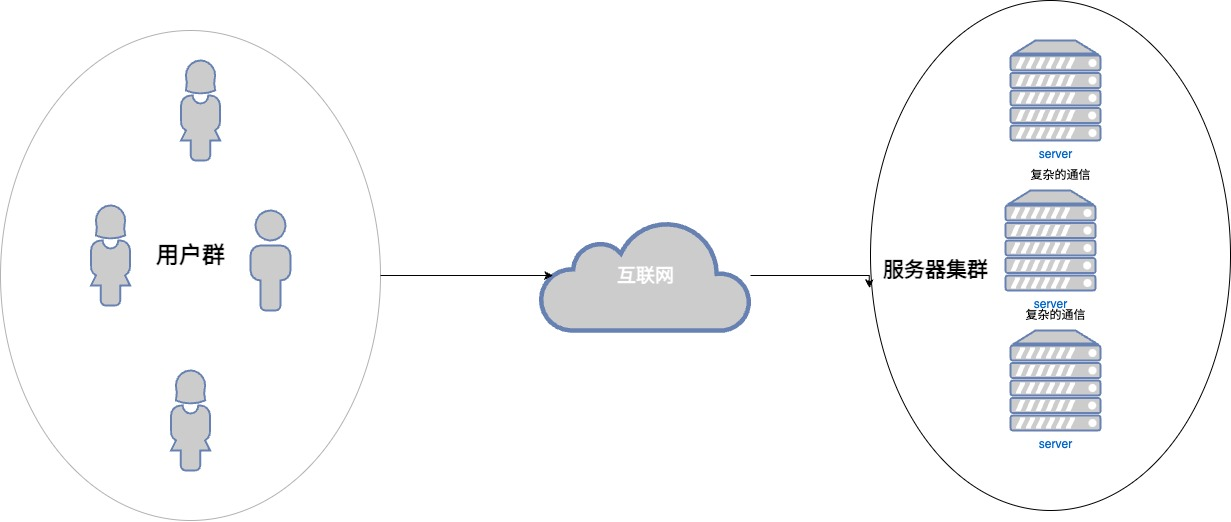
\includegraphics[width=\textwidth]{figures/cluster-and-client.jpg}
  \caption{服务器集群与客户端}
\end{figure}

\subsection{服务器集群的架构优势}

(1)高性能

服务器集群通过协调不同物理硬件性能的服务器,在服务器服务节点处理客户端的请求时,尤其是高并发的场景下,相比于
单个服务器而言,集群架构表现了优越的性能。这种优越的性能不仅仅是不同性能设备能力的叠加,更是因为通信细节的互相协作,紧密联系造就的。

(2)高可用

服务器集群的高可用性体现在服务器集群的容灾和故障转移之上\cite{刘金秀2019基于}。对于大型开发,企业业务来说,服务器的因为处理器负载过高或者其他
导致服务器出现问题而重启崩溃的问题是不可容忍的。集群能够处理这种单独服务器而引发的问题,即使集群中某个服务节点出现故障,
也不能够导致集群不可用,集群中其他服务节点需要立即分摊异常节点的工作。
而只有当集群中所有服务节点同时不可用时,集群才会停止服务。

(3)可伸缩性

可伸缩性实现了对服务器节点灵活管理,并且用户对此并无感知。在负载比较大的情境下,就需要增加对服务器节点的投入,相反
如果负载比较小的情景下,就可以减少集群内的服务器节点

而本文主要优化的方向就是可伸缩性方面,判断不同情境下可能的负载程度,通过对负载情况的预测,能够对实现可伸缩性较大程度的优化。

\subsection{服务器集群的分类}

服务器集群的分类标准有多种,依据不同的标准可以得到不同的集群类别。
例如以多业务结构划分集群,除去常见的同构集群类型外还有目前大量商用化的异构集群。
若以集群实际功能结构划分的话,有三类集群是比较常见的,依次是高性能计算集群、高可用集群以及负载均衡集群\cite{刘卓2017基于Nginx的负载均衡集群设计与实现}。

(1)高性能计算集群

目前高性能计算集一个分支,一直以来都在不断研究多机并行算法及相关软件的开发,
致力于打造超级计算机用于进行复杂的科学运算\cite{xuzongyu}。
通过使用并行计算技术,HPC集群将海量运算问题分解为若干个小部分进行独立运算,
最终结果将由各服务器的计算结果的汇总得到,即通过多台机器提高数据运算的能力,降低数据运算的时间成本。

伴随着当前大数据人工智能技术的发展,HPC集群已经逐渐渗透到科学研究的各个领域,给海量数据运算工作提供了强有力的保障。
高性能计算集群在地形分析、生物制药、数据挖掘以及图像处理等领域发挥着十分重要的作用

(2) 高可用集群

高可用集群顾名思义,即使在高负载、高并发的场景下,可以将该服务器中的服务、资源、IP等转移到另外一台服务器上,从而满足业务的持续性;这两台或多台服务器构成了服务器高可用集群。
简单来说就是京东淘宝24小时不断买买买,微信QQ不断发短信,保证了服务器的不间断运行。然而永远的不间断运行几乎是不可能的,常见的算法并不能彻底处理突然之间的高并发和高负载,比如在双十一期间,某购物网站无法处理突然增加的大量订单
用户刷新造成的DDoS行为,具体衡量标准请看下面这份表。

\noindent\begin{longtblr}[
  caption = {HA衡量标准\cite{信息安全技术信息系统灾难恢复规范}},
  ]{
    hlines,
    vlines,
    % colspec={|X[c]|X[c]|X[c]|X[c]|},
  }
    描述 & 通俗叫法 & 可用性级别 & 年度停机时间 \\
    基本可用性 & 2个9 & 99\% & 87.6小时 \\
    较高可用性 & 3 个9 & 99.9\% 8.8小时 \\
    具有故障自动恢复能力的可用性 & 4 个9 & 99.99\% & 53 分钟\\
    极高可用性 & 5 个9 & 99.999\% & 5 分钟 \\
\end{longtblr}

(3)负载均衡集群

当大量用户并发访问时,将请求转发到不同的机器止实现负载均衡。负载均衡集群是由前端的负载均衡器与后端的服务器构成负载均衡器
介于客户端和服务器之间,通过负载均衡调度策略将负载分发到后端服务器处理,负载均衡集群可以分散单台服务器的访问压力
和存储压力降低单台服务器宕机带来的业务影响\cite{吴宝花2020基于}。为了保证客户端发送的请求能够成功的发送给后端服务器。
处理负载均衡器会判断后端服务器是否正常可用,如果检查到后端服务器状态正常则根据相应的负载均衡策略从这些可用的服务器中选择一台服务器处理对应的请求,
但是如果检查到后端服务器状态异常,则该服务器会被自动剔除待其恢复正常再加入集群系统中。

\begin{figure}[ht]
  \centering
  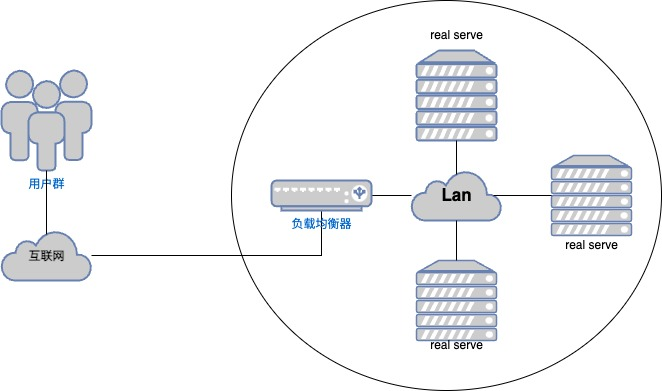
\includegraphics[width=12cm]{figures/负载均衡集群基本结构.jpg}
  \caption{负载均衡集群的基本架构}
\end{figure}

但是负载均衡集群存在一定的缺陷,负载均衡器无法对集群服务器性能进行监控,因而分配请求时容易导致服务器过载或者空闲情况的出现。
针对这种情况,该类集群将收集业务服务器动态负载状况的性能监控程序部署在请求分发服务器上,通过对该程序的使用可以时时刻刻掌握
上游服务器的负载变化。本论文的研究内容即是负载均衡集群下深度学习算法的使用。

\subsection{服务器性能指标}

负载均衡集群通过使用性能监控程序观察上游服务器的性能情况,要达到这一点,其中最主要的一点是如何选取评价节点当前负载状况的指标,且这些指标获取简单,获取时占用
系统资源少,更能有效的反映出的服务器节点的资源使用情况,可以将这些指标称作为负载向量。通过研究发现,反应服务器性能指标通常从这几个方面考虑:
CPU,内存,网络带宽,磁盘I/O,通过研究发现,采用不同的性能评价指标对负载均衡算法有较大的改变,而随着应用环境的改变,评价指标也会有不同的变化。

通过监控资源利用率(如 CPU、内存、磁盘 I/O 和网络带宽),系统可以确保工作负载均匀分布在所有可用资源上。
这样可以确保没有任何单个资源的过度使用,从而最大化整体性能。当业务增长时,可以根据资源利用率数据来决定何时需要
扩展硬件或调整系统配置,以优化性能和成本。

计算机一个重要的硬件就是 CPU,通常CPU的利用效率就几乎相当于服务器节点的性能情况,如果利用率过高,那么性能就会变低,
负载程度变大。每个 CPU 的大小核和频率也是影响 CPU 性能的重要组成条件,每个CPU的型号不同,那么需要将CPU性能作为负载向量的评价也就越难。
服务器节点的内存访问速率对 CPU 的任务处理效率影响较大。
而当网络请求量的增加带来的数据访问也会不断增加,在内存中数据请求和移动造成的分页错误或缺页的概率也会不断上升。
这样会严重影响CPU中任务处理效率,服务器节点处理请求任务的效率下降,导致集群整体的性能下降

如果主要对服务器的计算有着高性能的需求,那么最好将 CPU 和内存作为重要的评价指标,
若是处理的任务需要频繁的进行数据的传输和存储,那么网络和磁盘 I/O 对这种任务类型的影响更大。

上述负载向量指标只是服务器节点实时的工作状态\cite{mahato2017scheduling},而队列的长度是节点处理请求任务的,完成某项任务的整个流程法人方向来思考的,这种方式具有预测性的。
此时,如果有任务入队列,那么此时的服务器节点负载程度比较高,并不能接受更多的任务。性能监控程序只能监控当先服务器的实时性能,但是网络任务是作为队列被负载均衡器分发的
虽然能够判断队列的长度,但是队列里对任务消耗资源的能力是无法得知的,所以任务队列的长度不能准确反应节点的负载能力。队列一般考虑的是 CPU 的队列长度
获取 CPU 的队列长度,可以通过两个视角来呈现,其一是获取 CPU 一段时间内的平均队列长度,其二是获取 CPU 某个时刻的队列长度。

由于不能简单的使用 CPU 性能和任务队列长度作为负载向量指标,所以我们需要一个综合的负载信息评价标准,获取多种不同的指标信息,
经过数学运算,得到一个能够从多方面体现节点负载程度的新指标。通过对黄伟华,一种特征加权模糊聚类的负载均衡算法\cite{黄伟华2017一种特征加权模糊聚类的负载均衡算法}
 的研究,主要有三种方法。第一种方法既是使用队列长度作为主要指标,同时考虑使用 CPU 和磁盘IO 作为次要指标;另一种是完全结合,同时将队列的长度和资源利用
率作为参考指标;最后一种是通过优先级作为主要指标,比如内存占用情况,在内存充足的情况下,在考虑其他次要的指标。

\subsection{本文选择的参考指标}

依据自身经济和技术情况,选择使用观察节点的各种资源利用情况作为负载均衡能力的指标,并选取了 CPU,内存,磁盘 I/O 和网络带宽作为评价各个节点性能的指标。
具体的系统状态评价对应的资源利用率情况本文进行了整理,如下图表所示。

\noindent\begin{longtblr}[caption={稳定系统的资源状态和评价}]
  {hlines,vlines, colspec = {X[c]X[c]X[c]}}
  性能指标 & 资源利用率 & 状态评价 \\ 
  \SetCell[r=3]{c} CPU 利用率 & 70\% & 好 \\
                              & 85\% & 坏 \\
                              & 90\%+ & 很差 \\
  \SetCell[r=3]{c} 磁盘IO & <30\% & 好 \\
                          & <40\% & 坏 \\
                          & <50\% & 很差 \\
  运行队列 & <2*CPU数量 & 好 \\
  网络带宽 & <30\%带宽 & 好 \\
  \SetCell[r=3]{c} 内存 & 没有页交换 & 好 \\
                        & 每个 CPU每秒10个页交换 & 坏 \\
                        & 更多的页交换 & 很差\\
\end{longtblr}

设 $C_j$、$M_j$、$D_j$、$M_j$ 分别作为第 j 个节点的 CPU 剩余性能,内存剩余性能,磁盘剩余性能,网络带宽剩余性能。
在服务器集群处理大量任务和网络请求时,由于分发的请求量和请求所处理的数据量的不同,可能会出现有的节点处于高负载,
有的节点处于低负载的情况,这样服务器集群的性能就不能得到充分的发挥,所以需要一直监控集群中
各个节点的负载状况,不断调整任务队列的分配方案。下面是计算当前服务器节点的负载状态的数学公式
\[
  U_j = 1000 \cdot (W_{cpu} \cdot C_j + W_{mem} \cdot M_j + W_{io} \cdot D_j + W_{net} \cdot N_j)\tag{1.1}
\]
$U_j$ 为当前服务器节点的总体剩余性能。通过对 $U_j$ 值的监控,观察其变化范围作为判断是否需要修改请求人文分配方案的依据。

\section{负载均衡技术}

\subsection{什么是负载均衡}

负载均衡是在支持应用程序的资源池中平均分配网络流量的一种方法。现代应用程序必须同时处理数百万用户,并以快速、可靠的方式将正确的文本、视频、图像和其他数据返回给每个用户。为了处理如此高的流量,大多数应用程序都有许多资源服务器,它们之间包含很多重复数据。负载均衡器是位于用户与服务器组之间的设备,充当不可见的协调者,确保均等使用所有资源服务器。

\subsection{负载均衡的优势}

负载均衡可以定向和控制应用程序服务器与其访客或客户端之间的互联网流量。因此,它可提高应用程序的可用性、可扩展性、安全性和性能。

(1)应用程序可用性

服务器故障或维护可能会增加应用程序停机时间,使访客无法访问应用程序。
负载均衡器可以通过以下方式提高系统的容错能力,自动检测服务器问题并将客户端流量重定向到可用服务器。
运行应用程序服务器维护或升级而无需使应用程序停机,为备份站点提供自动灾难恢复,
执行运行状况检查并防止出现可能导致停机的问题。

(2)应用程序可扩展性

可以使用负载均衡器在多个服务器之间智能地定向网络流量。
应用程序可以处理数千个客户端请求,防止任何一台服务器出现流量瓶颈,
预测应用程序流量,以便可以在需要时添加或移除不同服务器,
为系统增加冗余度,使我们可以放心扩展。

(3)应用程序安全

负载均衡器具有多项内置的安全功能,它们是应对分布式拒绝服务攻击的有用工具,
在这种攻击中,攻击者会用数百万个并发请求淹没应用程序服务器,从而导致服务器故障。负载均衡能够做到:
监控流量并阻止恶意内容,预测应用程序流量,
将攻击流量自动重定向到多个后端服务器,以最大限度减少影响,
通过一组网络防火墙路由流量,以提高安全性。

(4)应用程序性能

负载均衡器通过增加响应时间和减少网络延迟来提高应用程序性能。它们可以执行诸如以下几项关键任务:
在服务器之间平均分配负载以提高应用程序性能,将客户端请求重定向到地理位置较近的服务器以减少延迟;
确保物理和虚拟计算资源的可靠性和性能。

\subsection{负载均衡的类型}

实现负载均衡的方式有很多种,最常见的时间负载均衡类型有三种。

(1)软件和硬件负载均衡

基于硬件的负载均衡器是一种硬件设备,可以安全地处理千兆字节的流量并将其重定向到数百个不同的服务器。可以将其存储在数据中心,并使用虚拟化创建多个可以集中管理的数字或虚拟负载均衡器。
基于软件的负载均衡器是执行所有负载均衡功能的应用程序。可以将它们安装在任何服务器上,也可作为完全托管的第三方服务的形式访问。

硬件负载均衡器需要初始投资、配置和持续维护。也可能不会满负荷使用它们,尤其只是为了处理高峰时段的流量高峰。如果流量突然增加到超出其当前容量,这将影响用户,
直到能购买并设置另一个负载均衡器为止。
相比之下,基于软件的负载均衡器要灵活得多\cite{常智2013高性能}。
它们可以轻松地纵向扩展或缩减,并且与现代云计算环境更加兼容。随着时间推移,它们的设置、管理和使用成本也会降低。

(2)静态和动态负载均衡

静态负载均衡是根据相关规则制定的负载均衡算法,典型的静态负载均衡策略有加权轮询、IP-HASH等。
静态负载均衡又称作确定性调度,这是由于在请求分发过程中该类策略不会考虑服务器实际运行时的负载性能,
这就容易导致出现性能好的服务器处于过载而性能一般的服务器处于轻载甚至空闲状态的不均衡状况,
集群资源利用率得不到充分发挥,系统性能被大大削减。静态负载均衡容易实现,配置简单,
因此也是比较常见且应用较多的一种负载均衡实现方式。

动态负载均衡的实现需要更为复杂的技术支撑,它在静态负载均衡的实现基础上,
需要对集群系统各服务器的运行状态加以评估,通过某些反映服务器运行时负载情况的负载评价指标的变化来动态调节各服务节点的请求分发比例,
从而能够将集群系统的资源充分利用在处理高并发客户端请求上,以达到集群负载动态均衡的目标。
在实践中,动态负载均衡能够大大提升集群系统的负载性能,但其实现是建立在一定量的系统资源消耗之上,对于一些没有资源的企业来说可能有点困难,但是对于大型企业来说这些成本就可以忽略不计。

根据负载均衡技术类型的不同,下表分析了常见的 Nginx 负载均衡策略。

\noindent\begin{longtblr}
  [caption = {常见 Nginx 负载均衡算法分析表}]
  {
    hlines,
    vlines,
    colspec = {X[c]X[c]X[l]X[l]},
  }
  负载均衡算法分类 & 算法名 & 优点 & 缺点 \\
  \SetCell[r=3]{c} 静态负载均衡 & 轮询算法 & 配置简单 & 不能考虑后端服务器性能差异 \\
                                & 加权轮询算法 & 能够考虑不同服务器的性能差异 & 不能考虑负载后服务器的状态变化 \\
                                & IP 哈希法 & 可以解决 session 问题 & 但在 Nginx 非最前服务器后失效 \\
  \SetCell[r=4]{c} 动态负载均衡 & 平均分配认为 & 不能考虑服务器处理能力不同 \\
                                & 加权最小连接法 & 考虑处理能力的不同 & 无法衡量服务器负载状态 \\
                                & 最短响应时间法 & 根据服务器响应时间分配请求 & 通信开销过大 \\
                                & 基于资源的方法 & 性能最大化,控制分散灵活 & 配置复杂,不一定反映实际负载 \\
\end{longtblr}

(3)四层到七层负载均衡

大型的网站服务一般会用这样的架构,在业务应用前面加七层负载均衡,然后在七层负载均衡前面加四层负载均衡。当用户发送 HTTP 请求的时候,请求会(经过机房内的路由器,交换机等设备)首先到达四层负载均衡,四层转发给七层,七层转发给应用。
四层负载均衡只解析网络包到第四层,根据四层的内容(比如 TCP port,IP 等)就能确定转发给谁,
七层负载均衡解析网络包到第七层,要根据七层的内容(比如 HTTP URL path,HTTP header 等)才能确定转发给谁。

七层即应用层\cite{pak2015efficient},要解析 HTTP 内容(不仅仅是 HTTP,其他应用层协议的负载均衡,比如一些数据库 proxy,gRPC 代理,等等,
都需要解析完成应用层才能确定转发目标),首先要将 Header 全部读完,读完之后要看下
Content Length 是有多长,然后知道 Body 要读到哪里。根据不同的 URL Path,
还要确定路由到哪一个 upstream。


四层即传输层,对于用户任务,四层负载均衡器首先通过预先配置好的负载均衡策略在内部网络
中挑选一台最好的服务器,接着将请求报文中的目标IP地址和端口号修改为内部最佳的服务器IP和端口号
并建立TCP链接转发请求,最后将响应结果返回给用户。用 Nginx 模拟四层负载均衡如下图所示。

\begin{figure}[htb]
  \centering
  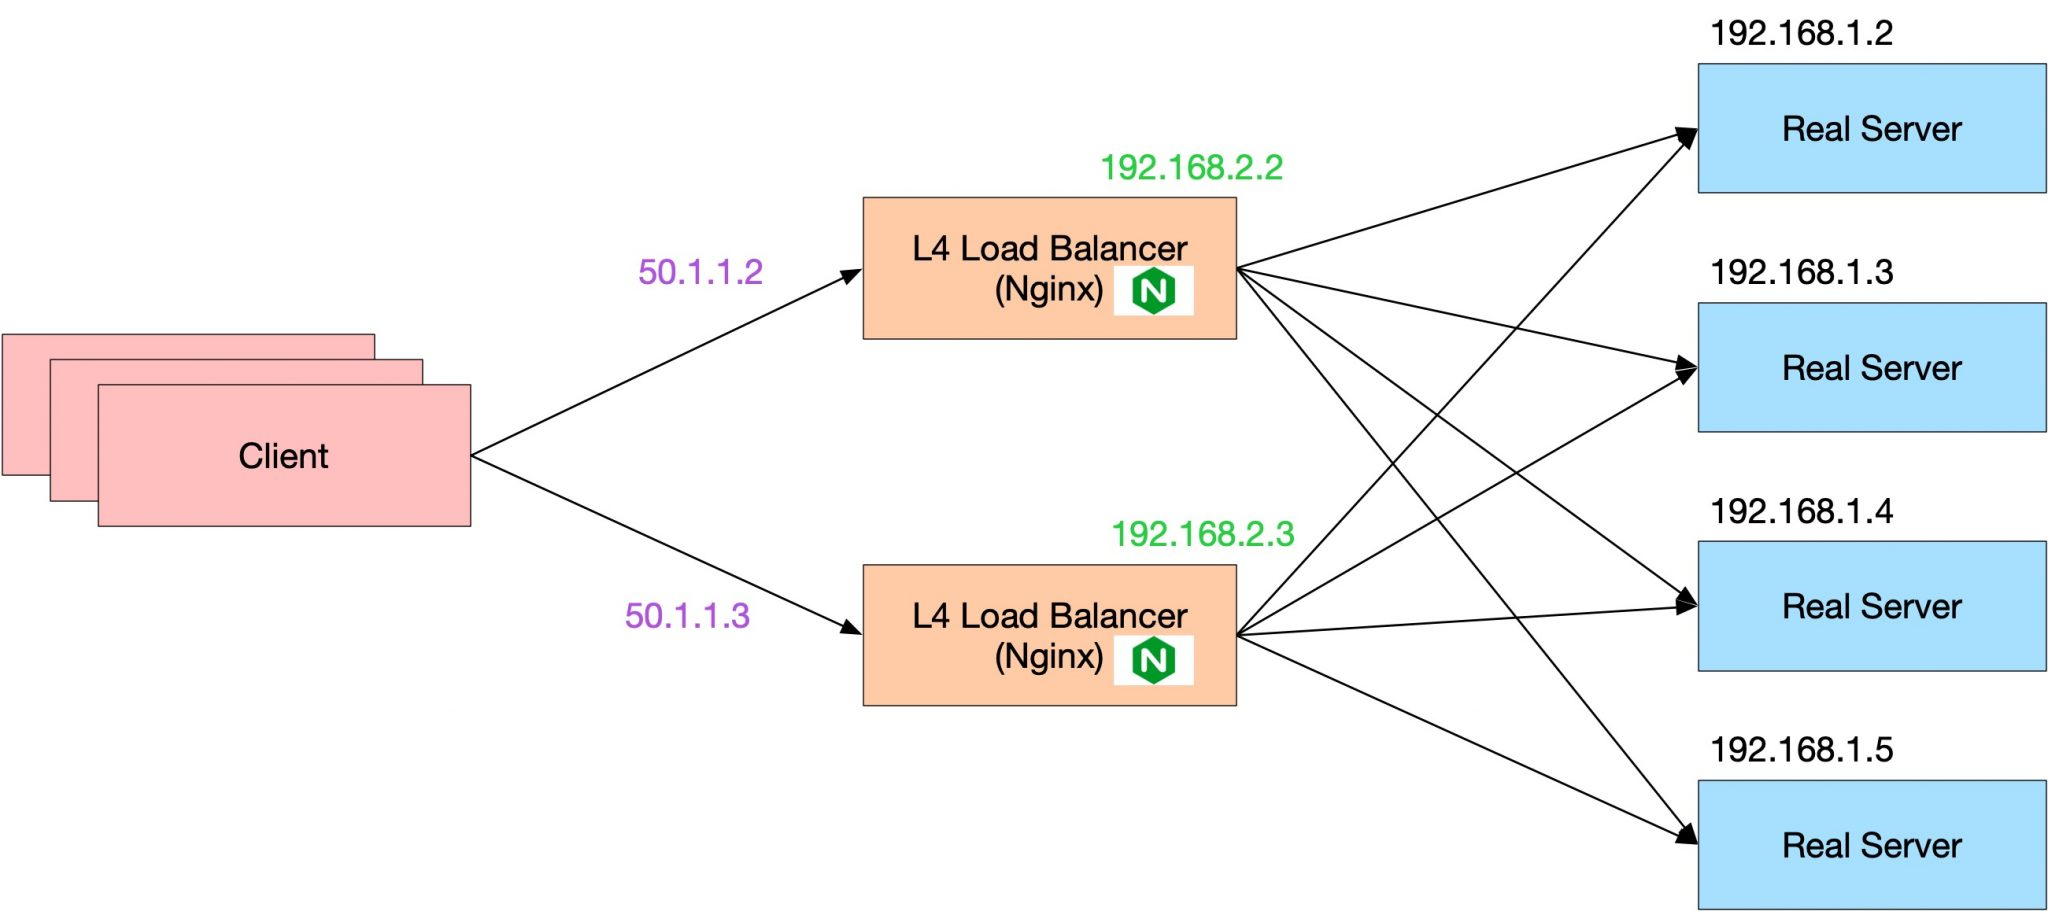
\includegraphics[width=\textwidth]{figures/nginx-l4lb-2048x911.jpg}
  \caption{Nginx 作为四层负载均衡使用}
\end{figure}

\newpage

\section{Nginx 服务器}

Nginx是一款轻量级的Web服务器/反向代理服务器及电子邮件代理服务器。本身具有占用内存少,并发能力强等特点,其并发能力在同类型的网页服务器中表现较好。
Nginx是由伊戈尔·赛索耶夫为俄罗斯访问量第二的Rambler.ru站点开发的,第一个公开版本0.1.0发布于2004年10月4日。
Nginx 相较于之前盛行的 LAMP(Linux Apache MySQL PHP/Python/Perl)由于 Apache 服务器同步多进程的处理方式,
而 Nginx 是基于事件驱动架构,在处理任务请求是异步而非阻塞的,因此应对高并发请求是以就能够保持资源的低消耗、响应能力迅速以及稳定性强的特点\cite{凌质亿2013高并发环境下}。包括百度,京东等众多服务器都是采用Nginx。

\subsection{Nginx 工作模式和进程模型}

Nginx 有单进程和多进程两种工作模式,默认进程为多进程。通常情况下,单进程仅仅只在开发环境下调试使用,对外发布服务时
常常使用多进程。多进程模型既是 master-worker 进程模型

\noindent\begin{enumerate}
  \item Nginx 启动后,会产生一个 master 主进程,主进程执行一系列的工作后会产生一个或者多个工作进程 worker
  \item 在客户端请求动态站点的过程中,Nginx 服务器还涉及和后端服务器的通信。Nginx 将接收到的 Web 请求通过代理转发到后端服务器,由后端服务器进行数据处理和组织
  \item Nginx 为了提高对请求的响应效率,降低网络压力,采用了缓存机制,将历史应答数据缓存到本地。保障对缓存文件的快速访问
\end{enumerate}

首先,worker 进程之间是平等的,每个 worker 进程都是从 master 进程 fork 过来,
在 master 进程里面,先建立好需要 listen 的 socket(listenfd)之后,
然后再 fork 出多个 worker 进程。每个 worker 进程,处理请求的机会也是一样的。
所有 worker 进程的 listenfd 会在新连接到来时变得可读,为保证只有一个进程处理该连接,
所有 worker 进程在注册 listenfd 读事件前抢 accept\_mutex,抢到互斥锁
的那个 worker 进程注册 listenfd 读事件,在读事件里调用 accept 接受该连接。
当一个 worker 进程在 accept 这个连接之后,就开始读取请求,解析请求,处理请求,产生数据后,
再返回给客户端,最后断开连接,这样就是一个完整的请求就是这样的了。

具体图示如下

\noindent\begin{figure}[htb]
  \centering
  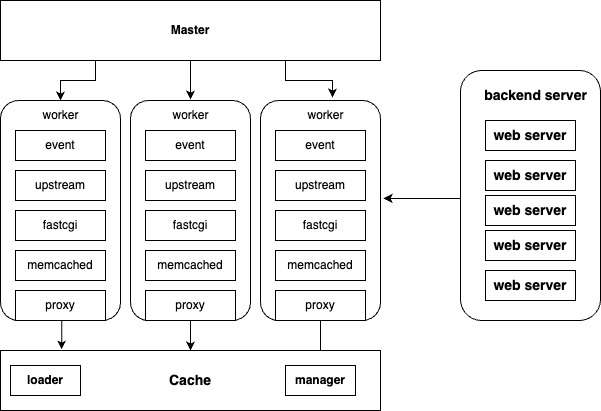
\includegraphics[width=0.8\textwidth]{figures/master-worker.jpg}
  \caption{Nginx 多进程工作模式}
\end{figure}

由于 Nginx 底层基于 epoil 事件驱动模型实现异步非阻塞 IO,一个进程可以监听多个 socket,因此每一个 worker 进程
都可以并发多个链接甚至上万个连接\cite{张炜森2018nginx},这保证了 Nginx 的高并发性能,而且消耗的内存非常少。

\subsection{Nginx的反向代理}

代理简单来说,就是如果我们想做什么,但又不想直接去做,那么这时候就找另外一个人帮我们去做。那么这个例子里面的中介公司就是给我们做代理服务的,我们委托中介公司帮我们找房子。
弄清楚代理是什么了,既然有反向代理,那么正向代理是什么?先从反向代理解释起。
反向代理,其实客户端是没有任何感知的,因为客户端不需要任何配置既可以访问。
我们只需要将请求发送到反向代理服务器,由反向代理服务器去选择目标服务器获取数据后,在返回给客户端,此时反向代理服务器和目标服务器对外就是一个服务器,暴露的是代理服务器地址,隐藏了真实服务器IP地址。

理解这两种代理的关键在于代理服务器所代理的对象是什么,正向代理代理的是客户端,我们需要在客户端进行一些代理的设置。而反向代理代理的是服务器,作为客户端的我们是无法感知到服务器的真实存在的。
总结起来就一句话:正向代理代理客户端,反向代理代理服务器\cite{崔娟2023基于Nginx反向代理解决公网上服务跨域问题的研究}。

用一个图片对比正向和反向代理

\begin{figure}[htb]
  \centering
  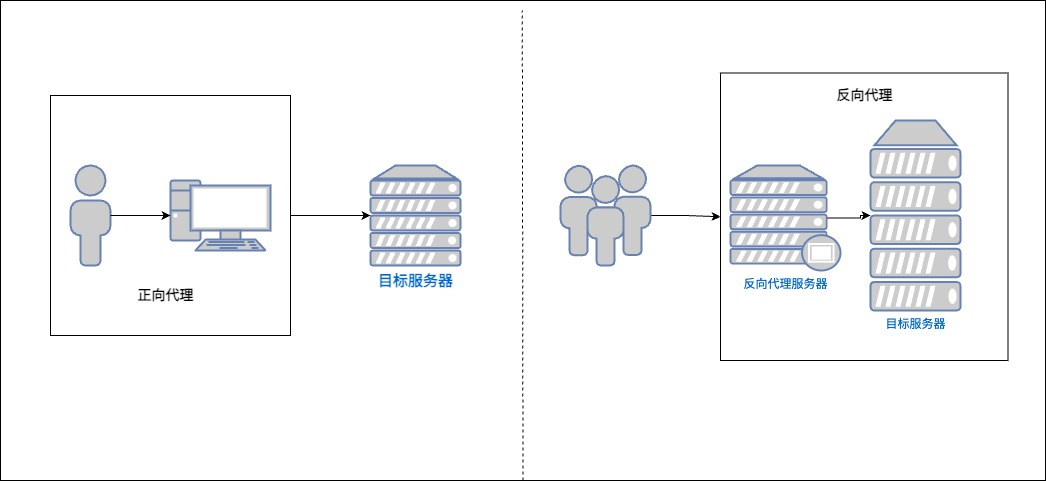
\includegraphics[width=\textwidth]{figures/Forward-Proxy-Reverse-Proxy.jpg}
  \caption{正向代理与反向代理的对比}
\end{figure}

Nginx反向代理功能使其能够逾越单机的局限性,并拥有在网络上接收、转发以及处理数据的能力\cite{马原龙2016nginx}。
通过proxy\_pass指令可以配置Nginx反向代理,proxy\_pass的语法结构为proxy\_passURL,
这个URL即表示Nginx所代理的上游服务器地址信息。
Nginx反向代理的一个配置实例如下所示,配置中的“proxy\_set\_headerX-Real-IP”表示定义了一个值为“\$remote\_addr”的首部“X-Real-IP”,
也即客户端的IP地址。当上游服务器接收到客户端请求时,该自定义的首部将以客户端IP的形式被打印到服务器访问日志中,
上游服务器便能够依据真实客户端的IP地址而非Nginx的IP地址做日志统计分析\cite{吴陈2020基于Nginx的服务器集群负载均衡策略的研究与改进}。

\newpage

\noindent \begin{lstlisting}[caption={Nginx 反向代理默认配置}]
location \index{
  set $upstream_url "";
  proxy_set_header X-Real-IP $remote_addr;
  rewrite_by_lua_file /home/${HOME}/luafile/log.lua
  proxy_pass http://upstream_url;
}
\end{lstlisting}

在客户端与 Nginx 通信过程中,当请求到达 Nginx 服务器时,Nginx 并不能立即与目标服务器建立 TCP 连接
而转发请求工作,而是将任务请求储存在内部缓存队列中,之后在与目标服务器通信发送请求,这种工作模式大大降低里服务器某一节点的负载压力。
另外,由于客户端与 Nginx 是在公网上进行网络通信传输,属于慢速连接,而 Nginx 与上游服务器一般是在内部网络进行通信,属于高速连接,考虑到 HTTP 连接具有无状
态性,客户端与 Nginx 可以开启 Keep-Alive 功能,Nginx 与上游服务器之间的 Keep-Alive
则可以关闭,因此更能将占用上游服务器的系统资源释放掉,进一步减轻服务器负载。

当上游服务器针对客户端HTTP请求处理结束并生成响应报文发送给Nginx反向代理服务器后,
Nginx首先将拆开报文进行相关处理,二次封装完成响应给客户端。
在这个过程中,Nginx是在接收上游服务器传来的响应报文的同时向客户端发送响应报文,
而不像客户端请求资源时Nginx先接收,接收完成后再发送给上游服务器的情况一样,
Nginx边接收边转发的工作模式可以极大地减小客户端响应的延迟\cite{邓仲举2012高可靠性集群部署的设计与实现}。

\subsection{Nginx 负载均衡}

Nginx 自身支持多种负载均衡算法,除了使用源码自带的内置调度算法之外,还可以支持第三方扩展的
负载均衡技术\cite{sufiev2016dynamic}。如果想要开启源码自带的调度算法可以则可以把指定调度算法
的模块打开。一般来说,不需要单独下载某一模块,需要使用时在配置文件中指定即可。Nginx 内置的调度
算法有加权轮询算法、最小连接算法、IP 哈希算法。第三方扩展算法则需要安装第三方模块,将模块放在指定的扩展算法
模块路径,在编译Nginx过程中,扩展算法会一并编译在二进制程序中,最后使用便可以依据配置指令使用指定的
第三方调度算法。常见的第三方调度算法有 fair 响应时间比算法(需要安装ngx\_http\_upstream\_fair\_module),URL 哈希算法(需要安装ngx\_http\_upstream\_hash\_module)
等。下面将对常见的Nginx调度算法进行分析。

(1)加权轮询算法

默认轮询算法(Round Robin)的策略是:将请求“依次”分发到候选机器。如下图所示,轮询负载均衡器收到来自客户端的 6 个请求,编号为 1、4 的请求会被发送到服务端 0;编号为 2、5 的请求会被发送到服务端 1;编号为 3、6 的请求会被发送到服务端 2。

\begin{figure}[htb]
  \centering
  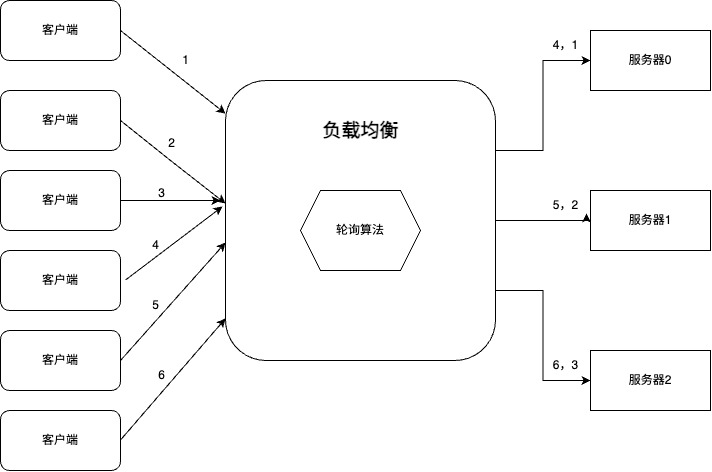
\includegraphics[width=\textwidth]{figures/round-robin.jpg}
  \caption{默认情况下的负载均衡算法}
\end{figure}

默认的轮询算法是等值轮询,即按照一比一的比例向不同的服务器节点分发请求,当配置文件
没有任何 weight 权值参数是,则采用默认的轮询算法。于是加权轮询算法则考虑了不同性能特点
的服务器节点,性能好的服务器则设置较大的权值,性能不好的服务器则设置较小的权值。
当任务入队列时负载均衡器则可以按照设置好的权值比例合理的悬着服务器执行请求调度

\begin{lstlisting}
# 默认的轮询算法
upstream backend {
    server 127.0.0.14:80 max_fails=2 fail_timeout=10s;
    server 127.0.0.15:80 max_fails=2 fail_timeout=10s;
}
# 加权轮询算法
upstream backend {
    server 127.0.0.14:80 weight=5 max_fails=2 fail_timeout=10s;
    server 127.0.0.15:80 weight=10 max_fails=2 fail_timeout=10s;
}
\end{lstlisting}

通过对 Nginx 源码的研究,在 ngx\_http\_upstream\_round\_round\_robin.c 这个文件下 ngx\_http\_upstream\_get\_round\_robin\_peer
函数是对加权轮询算法的实现。在具体分配任务的环节,为了记录上游集群节点服务器的权值公设有四个变量,
依次是 weight、effective\_weight、total 和 current\_weight。

\noindent\begin{longtblr}
  [caption = {加权轮询算法变量及描述}]
  {hlines, colspec = {|X[1, c]|X[2, c]|}}
  变量 & 描述 \\
  weight & 初始权值,固定不变 \\
  effective\_weight & 发生错误,权值减小 \\
  total & 集群服务器权值总和 \\
  current\_weight & 实时权值,初始为零 \\
\end{longtblr}

在一次任务中,负载均衡器勉励上游服务器节点的 current\_weight 加上起对应的有效权值 effective\_weight,
负载均衡器将会选择 current\_weight 最大的服务器节点为本轮最佳服务器。当该服务器正在进行任务时,负载均衡器会
降低其 current\_weight。Nginx 定义了两个事件状态,NGX\_OK 表示成功选择最佳服务器,NGX\_BUSY 表示服务器选择失败
或者通信发生错误。加权轮询算法详细流程如下图2.8 所示。

\begin{figure}[htb]
  \centering
  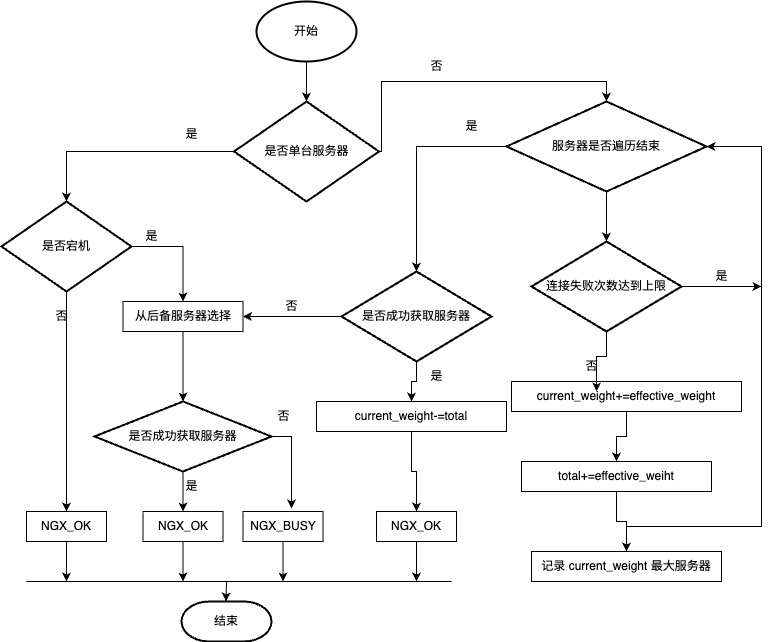
\includegraphics[width=\textwidth]{figures/round-flowchart.jpg}
  \caption{Nginx 加权轮询算法流程图}
\end{figure}

加权轮询算法,虽然考虑了上游服务器节点的不同性能差异,算法的复杂度比较低,执行效率较高,节点选择频次相对平滑,
配置简单,但是在具体任务过程中,有些任务比较繁忙,有些任务比较轻松,这种静态的权重调节无法根据真实负载
情况进行动态调整。为了解决这个问题,诞生了动态权值的加权轮询算法,基于手机各个后台服务器节点工作时的 CPU
利用率、内存利用率、网络性能和磁盘IO等性能情况,动态的调整后端服务器节点权重\cite{谭畅2021云中心基于}。该算法在高并发
的场景下,响应时间和实际并发方面表现更好。

(2)最小连接算法

最小连接算法(least\_conn)一句话概括就是:按nginx反向代理与后端服务器之间的连接数,连接数最少的优先分配\cite{周常志2023基于改进加权最小连接数的微服务负载均衡算法研究}。
要根据机器连接数分发,显然要先维护机器的连接数。
因此,最少连接数算法需要实时追踪每个候选机器的活跃连接数;
然后,动态选出连接数最少的机器,优先分发请求。最少连接数算法会记录当前时刻,
每个候选节点正在处理的连接数,然后选择连接数最小的节点。该策略能够动态、
实时地反应机器的当前状况,较为合理地将负责分配均匀,适用于对当前系统负载较为敏感的场景。

\begin{lstlisting}
# 最小连接算法
upstream backend {
    least_conn;
    server 127.0.0.14:80 max_fails=2 fail_timeout=10s;
    server 127.0.0.15:80 max_fails=2 fail_timeout=10s;
}
\end{lstlisting}

最小连接数调度算法每一个上游集群节点分别维护一个计数变量 number,每次负载均衡器分配个某一节点一个
任务时,就将其对应的 number 值上加上 1,当任务完成之后,再将 number 值减去 1。Nginx 根据集群各服务器
计数变量的变化,每次都会挑选 number 数值最小的服务器进行任务分配。同时最小连接算法与加权连接算法接轨,
如果初始为每一个性能各异的服务器分配初始权重,那么当分发任务请求时将选择连接数与权值比例最小的服务器
节点作为最佳服务器节点。最小连接算法流程图如下如下图所示。

\begin{figure}[htb]
  \centering
  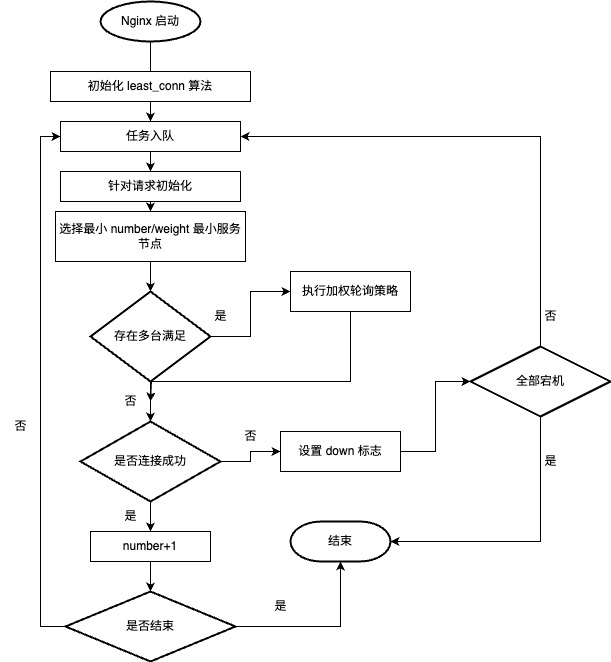
\includegraphics[width=\textwidth]{figures/least-flowchart.jpg}
  \caption{Nginx 最小连接算法}
\end{figure}

最小连接算法根据服务器连接数大小变化的统计结果来动态的选择服务器分发任务,对于服务器的实时
负载情况做了些许的考虑,一定程度上解决了加权轮询算法中请求到来时间间隔不一致所带来的负载差异。
但由于每条连接上的请求不同,该算法但从连接数大小来反应实时负载情况还是不够全面。

(3)IP 哈希算法

哈希算法(Hash)根据一个 key (可以是唯一 ID、IP、URL 等),通过哈希函数计算得到一个数值,用该数值在候选机器列表的进行取模运算,得到的结果便是选中的机器\cite{邱亚飞2021哈希算法的实现与验证}。
哈希算法解决的问题既是人工的判断某个具体任务需要的性能大小,如果该任务消耗的性能较多,负载均衡器将会对该请求连接进行分配到候选的高性能服务器中。
这种算法可以保证,同一关键字(IP 或 URL 等)的请求,始终会被转发到同一台机器上。哈希负载均衡算法常被用于实现会话粘滞(Sticky Session)。
但是 ,哈希算法的问题是:当增减节点时,由于哈希取模函数的基数发生变化,
会影响大部分的映射关系,从而导致之前的数据不可访问。要解决这个问题,
就必须根据新的计算公式迁移数据。显然,如果数据量很大的情况下,迁移成本很高;
并且,在迁移过程中,要保证业务平滑过渡,需要使用数据双写等较为复杂的技术手段。

\begin{figure}[htb]
  \centering
  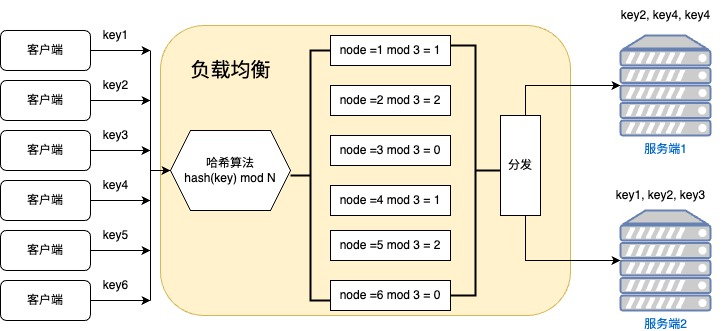
\includegraphics[width=\textwidth]{figures/hash-algo.jpg}
  \caption{Nginx 哈希算法拓扑图}
\end{figure}

Nginx 的IP 哈希算法则是将来源客户端的IP地址作为key,采用特定的哈希函数作哈希运算,最后将结果请求转发到特定的服务器上进行处理。
Nginx 负载均衡器受到客户端请求后,将该客户端的点分十进制前三段作为参数输入到哈希函数计算,哈希值的以保证 IP 地址前三段能够分发导通一个上游服务器,哈希
计算完成之后将此 hash 值 对集群中所有正常运行的服务器总数进行趋于,用来确定将任务请求分发到那台服务器上。在确定服务器节点过程中,
如果失败次数超过 20 次,将会替换为加权轮询策略。Nginx 配置 IP 哈希算法如下所示。

\begin{lstlisting}
# IP-HASH 算法
upstream backend {
    ip_hash;
    server 127.0.0.14:80 max_fails=2 fail_timeout=10s;
    server 127.0.0.15:80 max_fails=2 fail_timeout=10s;
}
\end{lstlisting}

IP 哈希算法流程图如下所示。

\begin{figure}[htb]
  \centering
  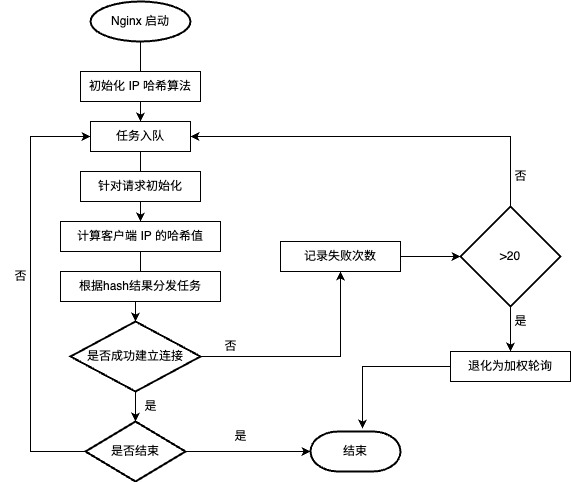
\includegraphics[width=\textwidth]{hash-flowchart.jpg}
  \caption{Nginx IP 哈希算法流程图}
\end{figure}

IP 哈希算法能满足用户会话保持的要求,因为同一个IP的用户请求将映射导通一个服务器节点进行处理。
当集群节点出现故障或者集群加入新节点,需要重新进行哈希运算,因此仍旧会出现会话沾性失效问题。
在资源占用率比较高的高并发情景下,IP 哈希算法对于不同资源的消耗仍旧无法考虑,还是容易导致某一个服务器节点过载而崩溃
而其他节点过于空闲的状态。所以任何不能彻底的明白每一个集群节点中的实时负载的负载均衡算法都无法保证节点是否过载或者过于空闲。

在上述的 Nginx 几种内置的常见调度算法,常见的扩展调度算法还有最小响应比算法。
fair 算法在分配客户端请求时依据上游服务器的响应时间作为参考量,将处理请求的高优先级赋予响应时间短的服务器,
由于响应时间越长的服务器负载相对越重,因此优先级滞后。fair 算法依据页面大小和加载时间长短能够自适应地进行负载均衡,
在一定程度上考虑到了上游服务器的性能差异。但在高并发情况下,没有考虑到网络拥塞可能带来的耗时延长的情况,
且单靠响应时间来判断负载过于片面,不够准确可靠\cite{张艳肖2023基于Fair函数神经网络的厚度传感器输出特性分析}。

经过上面的对Nginx几种内置的负载均衡算法可以得知,静态负载均衡算法配置一遍比较简单,而且执行效率很好,一定程度上能够反应集群节点的负载性能。
而动态负载均衡则配置比较复杂,在不考虑多方面的情况下,不够准确可靠,但是相比于静态负载均衡能够更加实时的了解某一节点的性能状态,以至于能够让
负载均衡器更好的分配工作。于是本文将从机器学习和神经网络方面探究动态负载均衡中关于网络方面的优化,并分析结果加以与原来对比。

\section{本章小结}

本章主要阐述了常规负载均衡算法探究涉及的相关理论和技术。首先介绍了服务器集群的概念和分类,
同时确定了如何测量服务器剩余节点性能的标准。其次分析了负载均衡技术的意义与优势,在分析负载均衡类型的过程中
确认了要突破的方向。最后通过对于Nginx 源码的了解探究了 Nginx 的工作模式和进程模型,了解了常规的负载均衡算法以及实现,
让我明确了向动态负载均衡算法中关于网络方面的研究方向。

%%================================================
%% Filename: chap03.tex
%% Encoding: UTF-8
%% Author: 苏峻锋
%% Created: 2024-02-28
%% Last modified: 2024-02-28
%%================================================
\chapter{网站访问量时间序列预测研究}

Nginx 作为一款高性能的HTTP和反向代理服务器,其本身和时间序列不是直接相关。
但是,在监控Nginx性能的过程中,会涉及到时间序列数据。比如,Nginx的访问日志和错误日志都会记录下请求的时间信息,
这些日志数据就构成了时间序列数据。可以通过分析这些时间序列数据来理解Nginx的流量模式、
性能趋势以及潜在的问题。而且,对于时间序列的处理和分析还可以应用在Nginx及其它服务的自动化监控和告警系统中。
这样的系统可以帮助管理者更有效地了解服务状态,并在出现问题时迅速作出反应。

\section{时间序列预测基本方法}

时间序列是一组按照时间顺序排列的数据点。这种数据点是通常按照固定的时间间隔收集,
比如每天,每周,每月,每年的观测值。间序列数据用在许多领域,包括经济学、气象学、社会学、工程和自然科学等。例如,股票市场价格、气温记录或公司收入都可以被视作时间序列数据。通过对时间序列数据的分析,可以洞察到数据背后的趋势、季节性变化、循环等特征,也可以用来做出未来的预测。
在 Nginx 网络访问量的时间序列数据点则可以将每一天某个网页的访问量记录下来,按照日期的对应关系,每一个 datetime 对应一个 record。

时间序列预测方法有很多,简单的方法不多提,主要研究了指数平滑法、趋势延伸法、自回归滑动平均模型(ARMA)、差分整合移动平均自回归模型(ARIMA)。

(1)指数平滑法。指数平滑法则在历史时间序列的数据给予权重之后的和作出了一些优化改进。
指数平滑法根据平滑的次数来进行分类,有一次指数平滑法、二次指数平滑法和三次指数平滑法等。
但它们的基本思想与移动平均法类似,都是历史时间序列的数据给予权重之后的和,但是它给不同的信息数据的权重大小不同,
与目标预测值时间距离越近,权重越大。
趋势延伸法主要趋势延伸法主要是将历史时间序列数据在坐标图上标记处所在的位置,
然后画出一条能最好反映历史数据变化的直线或者曲线,并进行延伸得到预测目标。

(2)自回归滑动平均模型\cite{贾钟研2020基于时间序列的网络流量分析与预测}(ARMA)
结合了自回归模型(AR)和滑动平均模型(MA),ARMA模型能有效地捕捉时间序列数据的自相关结构。
AR(p)模型,它预测当前值作为前p个观测值(lags)的线性组合,模型中的p代表模型的阶数,
即延迟的观测值的数量。AR部分的如下所示
\begin{equation}
  X_t = \phi_1X_{t-1} + \phi_2X_{t - 2} + \cdots + \phi_pX_{t-p} + \epsilon_t
\end{equation}
其中,$X-t$ 是时间序列在时刻 t 的值,$\phi_1, \phi_2,\ldots,\phi_p$是模型参数,$\epsilon_t$是白噪声误差项。
MA(q)模型,即移动平均模型,它使用当前和过去的预测误差(即观测值与模型预测值之间的差)来预测当前值。模型中的q代表误差项的阶数。
\begin{equation}
  X_t = \epsilon_t + \theta_1\epsilon_{t-1} + \theta_2\epsilon_{t-2} + \cdots + \theta_q\epsilon_{t-1}
\end{equation}
其中,$\epsilon_t$ 是模型的白噪声误差项,$\theta_1, \theta_2, \ldots, \theta_q$是模型参数。把AR部分和MA部分结合起来就得到了 ARMA 模型。
\begin{equation}
  X_t = \phi_1X_{t-1} + \cdots  + \phi_pX_{t-p} + \epsilon_t + \theta_1\epsilon_{t-1} + \cdots + \theta_q\epsilon_{t-q}
\end{equation}

ARMA模型的参数通常通过极大似然估计(Maximum Likelihood Estimation, MLE)或者最小二乘法来确定。在使用ARMA模型之前,往往需要确定模型的p和q值,这通常通过模型的自相关函数(ACF)和偏自相关函数(PACF)来辅助确定。此外,模型需要时间序列数据是平稳的,如果数据不平稳,往往需要通过差分等手段将其转化为平稳时间序列。

网络访问量的时间序列在一定时间内是比较平缓的,比如在每天的凌晨至第二天上午7点,七点到下午 5 点。这个时间点以外的访问量就比较复杂。遇见节日天气,访问量的预测就愈发困难。ARMA模型适合处理和预测短期的平稳时间序列数据,而在处理非平稳时间序列时,经常会使用ARMA模型的扩展版-ARIMA模型。

(3)自回归差分移动平均模型(ARIMA)。

ARIMA模型是在ARMA模型的基础上增加了差分的操作,以处理非平稳时间序列数据。ARIMA模型的一般形式为ARIMA(p, d, q)。其中,p是自回归项的阶数,d是差分次数,q是移动平均项的阶数。ARIMA模型的一般形式为
\begin{equation}
  (1 - \phi_1B - \cdots - \phi_pB^p)(1 - B)^dX_t = (1 + \theta_1B + \cdots + \theta_qB^q)\epsilon_t
\end{equation}

其中,B是差分操作符,$\phi_1, \phi_2, \ldots, \phi_p$是自回归项的系数,$\theta_1, \theta_2, \ldots, \theta_q$是移动平均项的系数,$\epsilon_t$是白噪声误差项。ARIMA模型的参数通常通过极大似然估计(Maximum Likelihood Estimation, MLE)或者最小二乘法来确定。在使用ARIMA模型之前,往往需要确定模型的p、d和q值,这通常通过模型的自相关函数(ACF)和偏自相关函数(PACF)来辅助确定。ARIMA模型的优点是能够处理非平稳时间序列数据,但是它的缺点是需要对模型的参数进行较为复杂的确定。

\section{访问量的时间序列预测算法}

对于访问量的预测能够有效的对服务器集群的负载能力加以调节,避免访问量过大导致的服务器集群某一节点的负载过高,使得任务处理能力下降,从而达到增强负载均衡的作用。

由于相关条件限制,未使用近几年的数据网页访问量数据作为原始数据。因此在此次预测模型测试中所使用的数据集为Kaggle比赛
“WebTrafficTimeSeries Forcasting”
所提供的的网络访问量数据集,该数据集收集了一些维基词条的日访问量情况,一共将近145000篇的维基百科页面。
train\_*.csv类型的文档包含了流量数据。其中每一行对应一篇特定的文章,每一列对应一个特定的日期。
train\_1.csv提供了从2015年7月到2016年12月一年多时间里共550天的的日访问情况,train\_2.csv提供了从2015年7月到2017年9月共803天的日访问情况。
key\_*.csv类型的文件提供用于预测的页名称和缩短的ID列之间的映射。

训练数据集由大约 145k 个时间序列组成。每个时间序列代表从 2015 年 7 月 1 日到 2016 年 12 月 31 日不同维基百科文章的每日浏览量。
每个时间序列,都有文章的名称以及该时间序列代表的流量类型(全部、移动、桌面、爬虫)。
此元数据和任何其他公开可用的数据来进行预测。缺点是该数据集的数据源不区分零流量值和缺失值。
缺失值可能意味着流量为零或当天的数据不可用。
本文采用了维基百科 “泰勒·斯威夫特” 词条的页面访问情况,如图3.1所示。

\begin{figure}[htb]
  \centering
  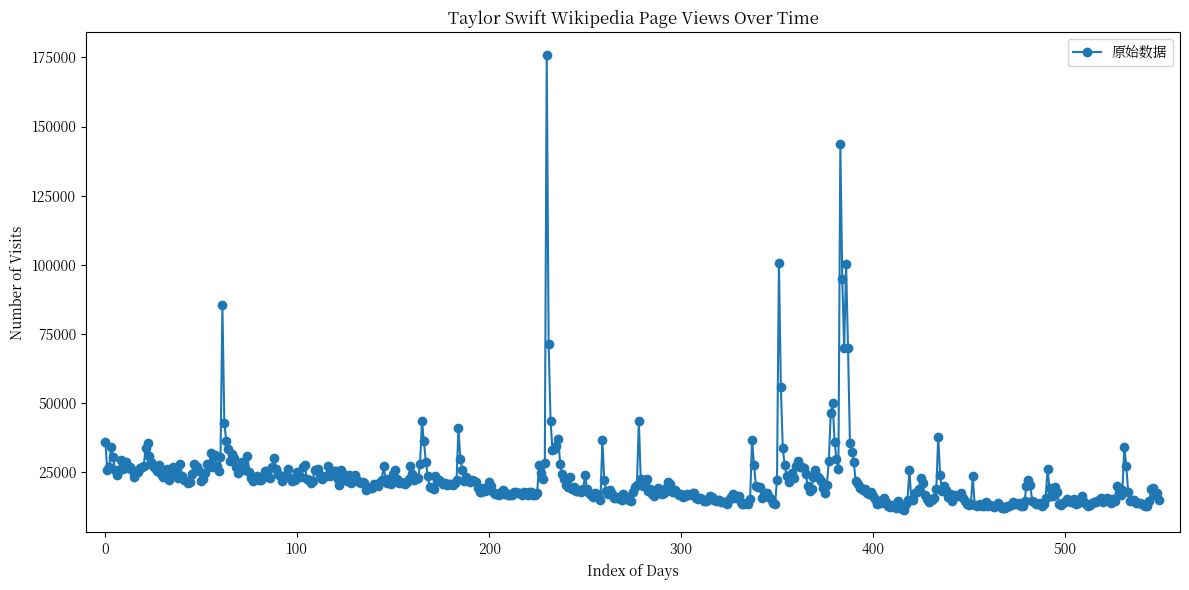
\includegraphics[width=\textwidth]{figures/taylor_source.png}
  \caption{泰勒·斯威夫特日访问量变化}
\end{figure}

为了能够知道模型的准确地,使用了重要指标 SMAPE(对称平均绝对百分比误差)一种常用于预测精度评估的指标,可以比较不同规模时间序列的误差。计算公式如下。

\begin{equation}
  SMAPE={\frac{100}{n}}\sum_{t=1}^{n}{\frac{|F_{t}-A_{t}|}{(|A_{t}|+|F_{t}|)/2}}
\end{equation}

其中这个公式的 $n$ 是观察总数,$F_t$ 是时间 t 的预测值,$A_t$ 是时间 t 的实际值。
SMAPE的值范围是0\%到200\%,较低的SMAPE值表示较高的预测精度。与其他评估指标相比,它同时考虑了预测值和实际值的误差,避免了过分强调其中一个
SMAPE通过相对误差进行测量,使其不依赖于数据的规模,因此适合比较不同规模的时间序列。

然而,SMAPE也存在一定的局限性,当时间序列的值接近零时,
SMAPE可以变得非常有问题。这是因为当实际值 ( A\_t ) 或预测值 ( F\_t ) 接近于零时,SMAPE的分母会变得很小,即使是很小的绝对误差也会导致很大的百分比误差。下面图3.2是关于 SAMPE 指标的极端测试图。

\begin{figure}
  \centering
  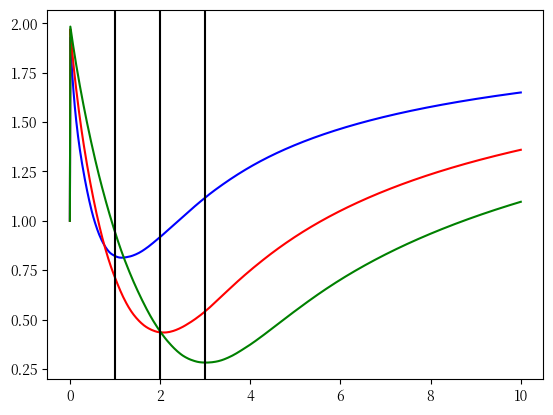
\includegraphics[width=0.8\textwidth]{figures/sampe_external.png}
  \caption{SAMPE 指标极端测试}
  \label{sampe-property}
\end{figure}

在图片\ref{sampe-property}中,垂直的线代表了真实值$1 , 2, 3$ 通过不同真实值的表现体现了 SAMPE 的动态分数。当实际值和预测值的差接近于零是,SMAPE 的分数会接近于无穷,所以要避免这个问题。

\subsection{ARIMA 算法访问量预测}

ARIME 模型也被称为 Box-Jenkins 模型,可能包含自回归项(AR)、移动平均(MA)、
差分运算(I)。

自回归即当前时刻的观察值是之前多个时刻观察值的线性组合加上一个随机误差项。
基本上,自回归的核心思想是,过去的值对未来的值有一定的预测能力,隐含地假设未来将与过去相似。
因为这个核心思想,所以必然的会有一定程度上的缺点。

移动平均(MA)是一种统计手段,用于分析时间序列数据。通过创建一系列平均数来平滑短期波动并突出显示长期趋势或周期。简单的举一个移动平均磨的模型,计算公式为 $SMA = \frac{P_1 + P_2 + \cdots + P_n}{n}$,其中P 是不同时间下的价格或者观察的序列,
而 n 是时间周期的长度即周期内一共有多少观察的时间数目

差分运算(I)是在时间序列分析中用于使非平稳的时间序列数据变得平稳的一种方法。如果一个时间序列是平稳地,意味着它的统计特性(均值、方差)不随着时间的变化。
平稳性是许多统计模型和预测方法的重要前提,非平稳时间序列可以通过差分变成平稳序列,这就是差分运算的作用。差分运算的基本形式是计算时间序列中连续观测值之间的差异。
举个例子,一阶差分的计算公式为 $\Delta Y_t = Y_t - Y_{t - 1}$,很好理解,如果一阶差分的时间序列不平稳,则可以进行更高级的差分,比如二阶差分:
\begin{equation}
  \Delta^2 Y_t = (Y_t - Y_{t - 1}) - (Y_{t - 1} - Y_{t - 2})
\end{equation}

一般来说,一阶或二阶差分足以处理大多数的非平稳序列。差分运算是构建ARIMA(自回归积分滑动平均)模型的关键步骤之一

对于 ARIMA 模型来说,可以通过上面三个关键含义来理解这个模型。自回归是指显示变化变量的模型,该变量根据自身的滞后值或者先验值进行回归;差分,表示
原始观测值与先前值的差异,用来使时间序列变得平稳;移动平均结合了观测值与应用于滞后的观测值的移动平均模型之间的残差之间的依赖性

(1)数据的预处理

由于 Kaggle 比赛中使用的数据命名的混乱,比如存在 52\_Hz\_I\_Love\_You\_zh.wikipedia.org\_all-access\_spider 
复杂的命名需要进行重新命名和分类,同时需要填充不存在的数值为 NaN
同时由于 ARIMA 模型对数据进行分析和预测要求序列是有一个零均值平稳随机过程产生,因此需要需要判断数据的平稳性\cite{赵鹏2020基于},通过使用 ADF 检验序列中是否存在单位根,如果存在则为非平稳时间序列。
ADF检验的核心是基于一个时间序列模型来测试序列中的单位根。具体来说,ADF检验通常使用以下的回归模型来进行单位根的测试。
\begin{equation}
    \Delta y_t = \alpha + \beta t + \gamma y_{t-1} + \delta_1 \Delta y_{t-1} + \cdots + \delta_p \Delta y_{t-p} + \epsilon_t
\end{equation}
在这个公式中,$y_t$ 是时间序列数据,$\Delta$ 是一阶差分运算符,$\Delta y_t = y_t - y_{t-1}$,$t$ 是趋势项,$\alpha$是常数项,$\beta$ 是时间趋势项的系数,$\gamma$ 是滞后一阶的系数,ADF检验的关键在于检验这个系数;如果$\gamma = 0$,则存在单位根,$\delta_1, \delta_2, \cdots, \delta_p$ 是差分项的系数,$\epsilon_t$ 是随机误差项,$p$ 是滞后阶数,它可以根据各种信息准则(如AIC或BIC)来确定。下表给出了泰勒·斯威夫特词条进行ADF检验的结果。

\noindent\begin{longtblr}[
  caption = {泰勒·斯威夫特的 ADF 检验},
]{
  width = \linewidth,
  colspec = {Q[312]Q[279]Q[410]},
  cell{1}{1} = {c=2}{0.591\linewidth,c},
  cell{2}{1} = {r=3}{},
  cell{5}{1} = {c=2}{0.591\linewidth,c},
  cell{6}{1} = {c=2}{0.591\linewidth,c},
  hline{1,7} = {-}{0.08em},
  hline{2} = {-}{},
}
参数    &            & 值             \\
测试临界值 & level 1\%  & -3.442361e+00 \\
      & level 5\%  & -2.866838e+00 \\
      & level 10\% & -2.569592e+00 \\
t统计量  &            & -7.674316e+00 \\
P 值   &            & 1.563457e-11  
\end{longtblr}

ADF 的检验结果可知,
ADF 值即 t 统计量远远小于 level 1\%、level 5\%、level 10\%的三个显著性水平条件下的临界值,故该原始序列为平稳时间序列,非常适合 ARIMA 模型来进行预测。

(2)参数标定

根据 ADF 的检验结果得知,该时间序列是一个平稳的时间序列,已经不需要进行差分,所以参数 d 即原始观测值差异的次数;也称为差异度为 0。
而 q 和 p 的数值则需要通过自相关及偏自相关函数来进行判断。

在时间序列分析中,p和 q 是ARIMA模型(自回归差分移动平均模型)的关键参数\cite{TJJC201923008},
其中p代表自回归(AR)项的阶数,它是过去值的数量, q代表移动平均(MA)项的阶数,它是预测误差的数量。
为了得到合适的 p 和 q 值,自相关函数(ACF)为移动平均组件 q 提供界限。ACF 图显示了时序和它自己滞后版本之间的相关性。
偏自相关函数(PACF):为自回归组件 p 提供界限。PACF 图仅显示不被更早滞后项解释的当前滞后项的相关性。自相关和偏自相关函数系数和滞后值关系如下:

\begin{figure}[htb]
  \centering
  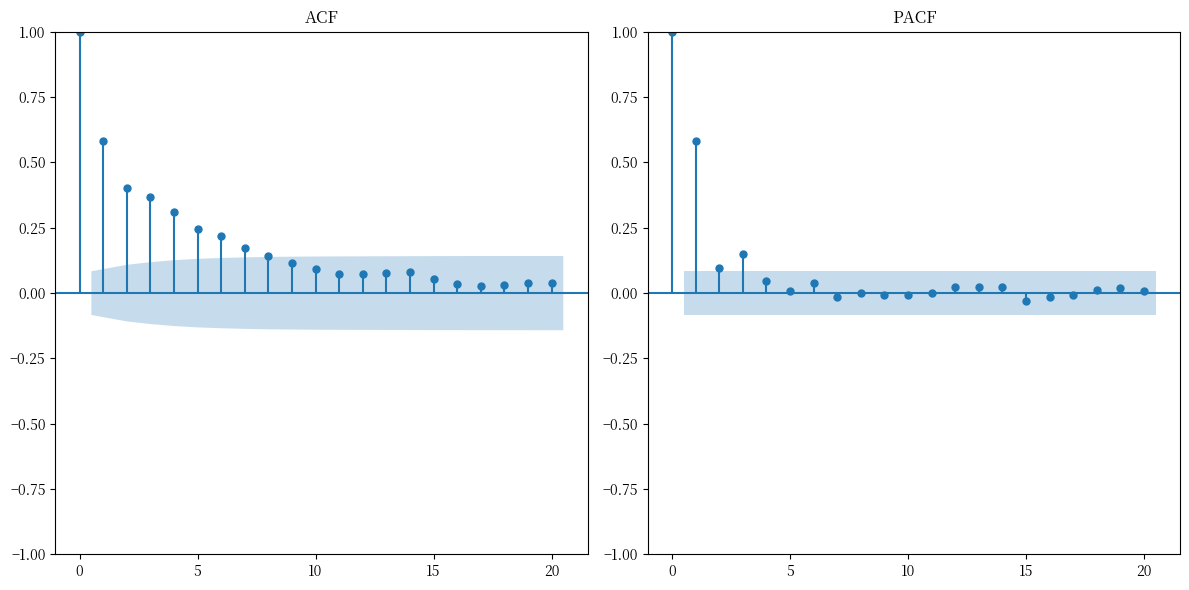
\includegraphics[width=\textwidth]{figures/acf_pacf.png}
  \caption{ACF 与 PACF 相关系数和滞后值的联系}
\end{figure}

如图3.2 所示,x 值即滞后值,y 值即相关系数,蓝色的区域是显著性水平分界线,如果在蓝色之内则是非显著的,
因为我们必须要对数据具有显著性的要求,毕竟如果没有显著性的差异,也就很难有什么变化或者预测了。ACF 图和 PACF 表示的是一个 AR 过程和 MA 过程一个相关性不断减小的过程。
当PACF图在滞后数p之后截尾,即相关性突然下降到不显著水平,则可以用来辨识AR模型的阶数p即为2; 当ACF图在滞后数q之后截尾即相关性突然下降到不显著水平,则可以用来辨识MA模型的阶数q 即为 1。利用 Python 对该模型的个参数进行估计,得到参数估计结果见表3.6。

\noindent\begin{longtblr}[
  caption = {ARIMA 模型拟合结果},
]{
  width = \linewidth,
  colspec = {Q[292]Q[173]Q[237]Q[173]},
  hline{1,6} = {-}{0.08em},
  hline{2} = {-}{},
}
模型     & 系数    & t 统计量   & P 值   \\
AR(1)  & 0.169 & 6.796   & 0.000 \\
AR(2)  & 0.107 & -2.310  & 0.021 \\
MA(1)  & 0.163 & -4.059  & 0.000 \\
SMA(2) & 3.086 & 3.4e+07 & 0.000 
\end{longtblr}

其中 $p$ 值是一个统计假设检验的概念,帮助决定观察到的数据是否显著性的与假设矛盾,进而否定这个假设。如果 $p$ 值很小,小于 0.05 那么就说结果具有统计学上的显著性,这表示出现极端数据的概率很低,反之则没有统计学上的相关性,很难找到统计学上的意义。
可以看出 ARIMA(2,0,1)在 1\%的显著水平下,AR(1)、AR(2)、MA(1)、SMA(2)的相关系数显著不为 0,回归系数的 $p$ 值均小于 0.05,所以对于 泰勒斯威夫特这个词条,通过了显著性检验。

已经确定了 $p$, $d$, $q$, 的值,则可以直接对泰勒·斯威夫特的时间进行预测,图3.4 是泰勒·斯威夫特的ARIMA预测值与实际值的对比。

\begin{figure}[htb]
  \centering
  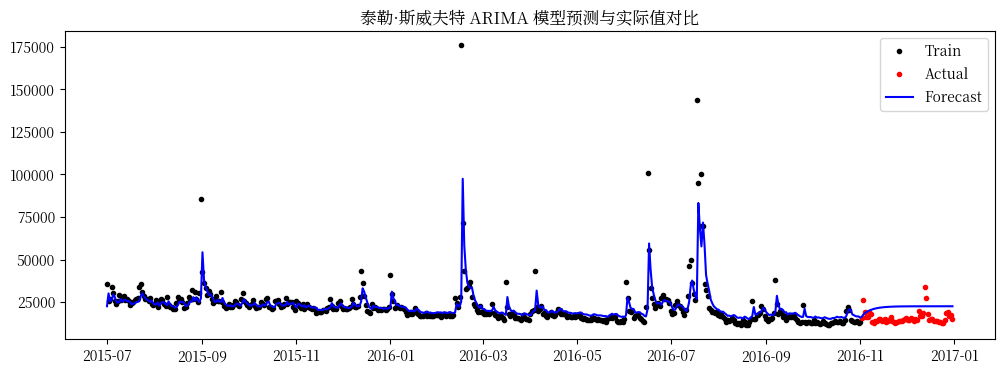
\includegraphics[width=\textwidth]{figures/taylor_arima.png}
  \caption{泰勒·斯威夫特词条 ARIMA 模型预测结果}
\end{figure}

可以看到蓝色的线条基本覆盖掉原始的训练实际值,但是在使用拟合的模型来进行预测的时候,可以看到蓝色的线条并不能很好的覆盖掉真实的实际值即模型仍旧没有很好的预测到真实的实际情况,需要进一步的分析研究。

在某些场景下,ARIMA模型通常被认为是适用于短期预测的,自回归部分依赖于时间序列的先前值,而移动平均则依赖于预测误差的先前值。因此,模型特别关注数据中的局部波动,而这些往往在短期内更加稳定。
但是在长期预测场景下,可能存在许多不可预测的外部因素和趋势变化,这些因素很难被ARIMA模型所捕捉。为了解决上述问题,让时间序列更好的得到预测,笔者使用了 Facebook 的 prophet 模型对词条进行预测。

\subsection{Facebook prophet 算法访问量预测}

Facebook的Prophet模型是一个开源的时间序列预测工具,由Facebook的Core Data Science团队开发\cite{taylor2018forecasting}。
Prophet的设计目标是让时间序列的预测工作变得更加简单,并且它对于具有强季节性效应的历史数据尤其适用。
它在处理缺失数据和异常值方面具有鲁棒性,并且能容忍时间序列中的一些非常规变化,因此对实际应用场景非常友好。此外,Prophet还支持添加重要的节假日效应。

Prophet模型在使用上很灵活,使得用户可以根据自己的需求和熟悉的环境来选择合适的工具进行预测。
Prophet背后的模型基础是一个可加性模型,其中趋势、季节性和节假日效应可以分解非常清晰地展示出来,这使得模型的结果很容易解释。

在时间序列分析领域,有一种常见的分析方法叫做时间序列的分解(Decomposition of Time Series),
它把时间序列 $y_t$ 分成几个部分,分别是季节项 $S_t$ 趋势项 $T_{t}$ ,剩余项 $R_{t}$;
一般来说,在实际生活和生产环节中,除了季节项,趋势项,剩余项之外,通常还有节假日的效应。所以,
在 prophet 算法里面,作者同时考虑了以上四项,也就是:$y(t) = g(t) + s(t) + h(t) + \epsilon_{t}$ 

其中 $g(t)$ 表示趋势项,它表示时间序列在非周期上面的变化趋势;$s(t)$ 表示周期项,或者称为季节项,
一般来说是以周或者年为单位;$h(t)$ 表示节假日项,表示在当天是否存在节假日;$\epsilon_{t}$ 表示误差项或者称为剩余项。Prophet 算法就是通过拟合这几项,然后最后把它们累加起来就得到了时间序列的预测值。

(1)趋势项 $g(t)$

在 Prophet 算法里面,趋势项有两个重要的函数,一个是基于逻辑回归函数(logistic function)的,
另一个是基于分段线性函数(piecewise linear function)的。

在逻辑回归函数中,一般形式是 $\sigma(x) = 1/(1+e^{-x})$ ,它的导数是 $\sigma'(x) = \sigma(x) \cdot(1-\sigma(x))$,而且$\lim_{x\rightarrow +\infty} \sigma(x) = 1, \lim_{x\rightarrow -\infty} \sigma(x) = 0$。
如果增加一些参数的话,那么逻辑回归就可以改写成如下方程\cite{李威2021Prophet模型在GNSS坐标时间序列中的插值分析} 。
\begin{equation}
  g(t) = \frac{C}{1 + e^{-k(t - m)}}
\end{equation}
方程式中,$C$ 是曲线的最大渐进值,即 $g(t)$ 随着时间增加越来趋向于 $C$;$k$ 为曲线的增长率;m 为曲线的偏移量。
但是在现实环境中,函数$g(t) = \frac{C}{1 + e^{-k(t - m)}}$的三个参数 $C, k, m$ 不可能都是常数,而很有可能是随着时间的迁移而变化的,因此,在 Prophet 里面,作者考虑把这三个参数全部换成了随着时间而变化的函数,也就是$C = C(t), k = k(t), m = m(t)$。
在现实的时间序列中,曲线的走势肯定不会一直保持不变,在某些特定的时候或者有着某种潜在的周期曲线会发生变化,这种时候,就有学者会去研究变点检测

假设已经放置了 $S$ 个变点,并且变点的位置是在时间戳 $s_{j}, 1\leq j\leq S$ 上,在这些时间戳上,我们就需要给出增长率的变化。
如果一开始的增长率我们使用$k$ 来代替的话,那么在时间戳$t$ 上的增长率就是$k + \sum_{j:t>s_{j}} \delta_{j}$ 通过一个指示函数 $\mathbf{a}(t)\in \{0,1\}^{S}$
那么在逻辑回归函数的形式如下,其中 $\mathbf{a}(t) = (a_{1}(t),\cdots,a_{S}(t))^{T},  \mathbf{\delta} = (\delta_{1},\cdots,\delta_{S})^{T}, \mathbf{\gamma} = (\gamma_{1},\cdots,\gamma_{S})^{T}$。
\begin{equation}
  g(t) = \frac{C(t)}{1+\exp(-(k+\mathbf{a}(t)^{t}\mathbf{\delta}) \cdot (t - (m+\mathbf{a}(t)^{T}\mathbf{\gamma})}
\end{equation}

在prophet程序里面有两种方法,一种是通过人工指定的方式指定变点的位置;另外一种是通过算法来自动选择。
在默认的函数里面,Prophet 会选择 n\_changepoints = 25 个变点,然后设置变点的范围是前 80\%(changepoint\_range),也就是在时间序列的前 80\% 的区间内会设置变点。

在分段线性函数的趋势项中,在每一个子区间上,函数都是线性函数,但是在整段区间上,函数并不完全是线性的。故根据变点的位置和变化量之间的关系,得出的分段线性函数如下。
\begin{equation}
  g(t) = (k + \mathbf{a}(t)\mathbf{\delta}) \cdot t + (m + \mathbf{a}(t)^T\mathbf{\gamma})
\end{equation}

其中$k$ 表示全局增长率(growth rate),$\delta$ 表示增长率的变化量,$m$ 表示偏移量,$a(t)$ 是一个向量,其中的每一项在t小于突变点时为0,在突变点之后为1。
而这两种方法(分段线性函数与逻辑回归函数)最大的区别就是 $\gamma$ 的设置,在分段线性函数中,$\gamma$ 是校正项,
其定义为在突变点上的增长率乘以突变点的时间即 $\gamma=(\gamma_{1},\cdots,\gamma_{S})^{T}$,$\gamma_{j}=-s_{j}\delta_{j}$ 

针对泰勒·斯威夫特词条的数据,在趋势项中没有什么值得改变的,顶多需要指定一下变点的位置,本文选择使用程序算法自己选择。

(2)季节项 $s(t)$

几乎所有的时间序列预测模型都会考虑这个因素,因为时间序列通常会随着天,周,月,年等季节性的变化而呈现季节性的变化,也称为周期性的变化。
在论文中\cite{taylor2018forecasting},作者使用傅立叶级数来模拟时间序列的周期性,当$T = 7, N = 3$ 时,表示以周为周期,当$T = 362.25, N = 10$ 表示以年为周期。
\begin{equation}
  s(t) = \sum_{n=1}^{N}\bigg( a_{n}\cos\bigg(\frac{2\pi n t}{P}\bigg) + b_{n}\sin\bigg(\frac{2\pi n t}{P}\bigg)\bigg)
\end{equation}

下图\ref{Trend-decomposition}是对泰勒·斯威夫特词条时间序列的趋势分解图,包括趋势,季节性,残差,经过趋势分解,发现并没有明显的季节性因素
。

\begin{figure}[htb]
  \centering
  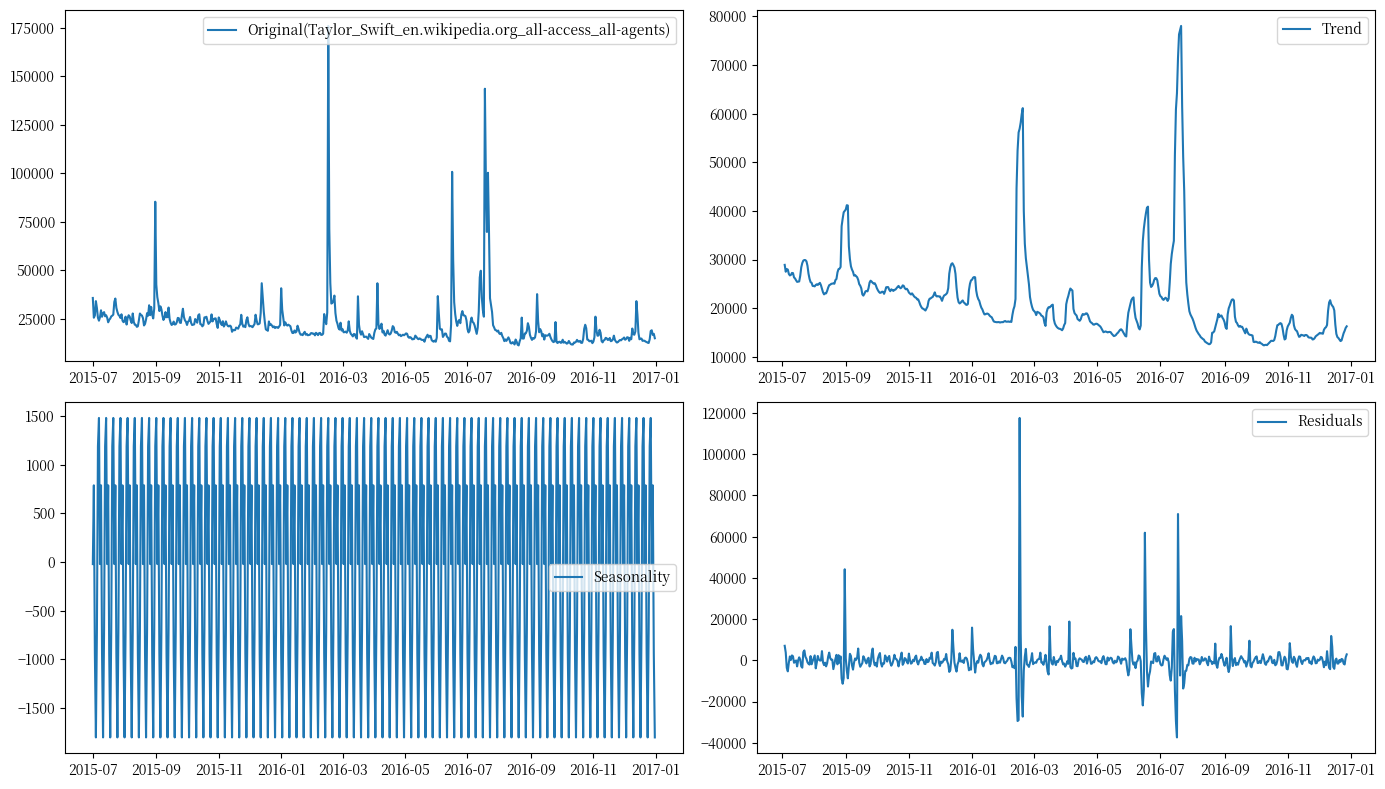
\includegraphics[width=\textwidth]{figures/Trend-decomposition.png}
  \caption{泰勒·斯威夫特趋势分解}
  \label{Trend-decomposition}
\end{figure}

(3) 假日项以及特殊因素

$h(t)$可用来反映时间序列中某时刻的特殊变动,Prophet模型根据每个假日项在不同时刻下产生的影响构建独立的模型,
并为各个假日项设置不同的前后窗口期,以及产生相应的虚拟变量\cite{JSJA2019S1097}。$h(t)$ 的表达形式如下。
\begin{align}
  h(t)&=\sum_{i=1}^{L}K_{i}1\ (t\in D_{i}), \\
  Z(t)&=[1(t\in D_{1}),...,1\ (t\in D_{L})], \\
  h(t)&=Z(t)_{k},k\sim normal(0, \gamma)
\end{align}

在现实环境中,除了周末,同样有很多节假日,而且不同的国家有着不同的假期。
在 Prophet 里面,通过维基百科里面对各个国家的节假日的描述,hdays.py 收集了各个国家的特殊节假日。
针对泰勒·斯威夫特这个词条来说,每一次专辑的发售都是一次重要的影响,发售专辑的时间可以算做一个假日。

通过加上不同影响因素,模型的准确度也会不一样。笔者通过加上不同的选项比如周期性,假日性和普通 prophet 模型加以对比,选出了效果比较好的一个模型。

\begin{figure}[htbp]
\centering
\begin{subfigure}{.5\textwidth}
  \centering
  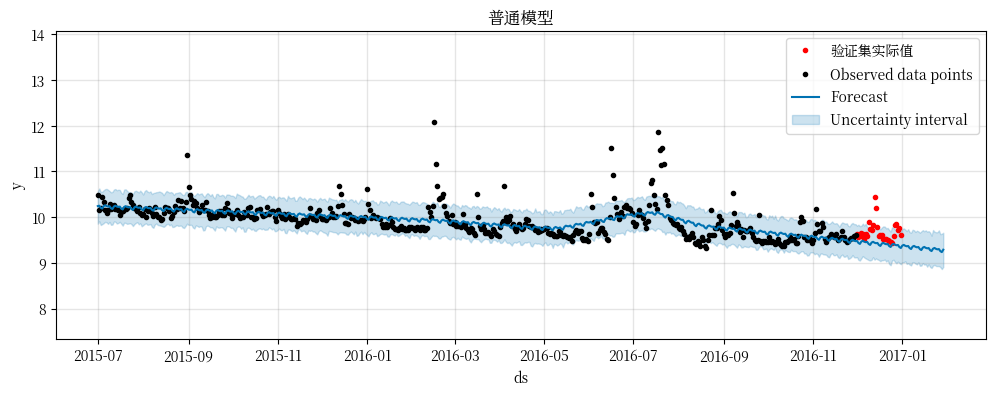
\includegraphics[width=\linewidth]{figures/prophet_normal.png}
  \caption{ProPhet 普通模型}
\end{subfigure}%
\begin{subfigure}{.5\textwidth}
  \centering
  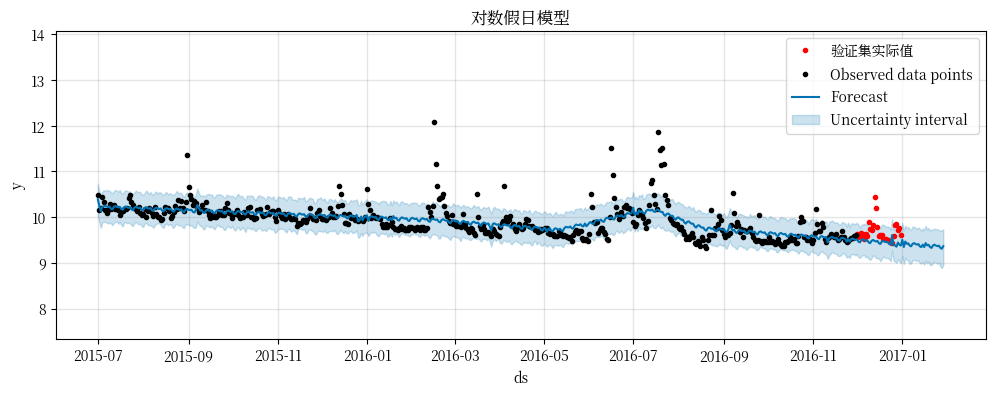
\includegraphics[width=\linewidth]{figures/prophet_holidays.png}
  \caption{Prophet 假日模型}
\end{subfigure}\\
\begin{subfigure}{\textwidth}
  \centering
  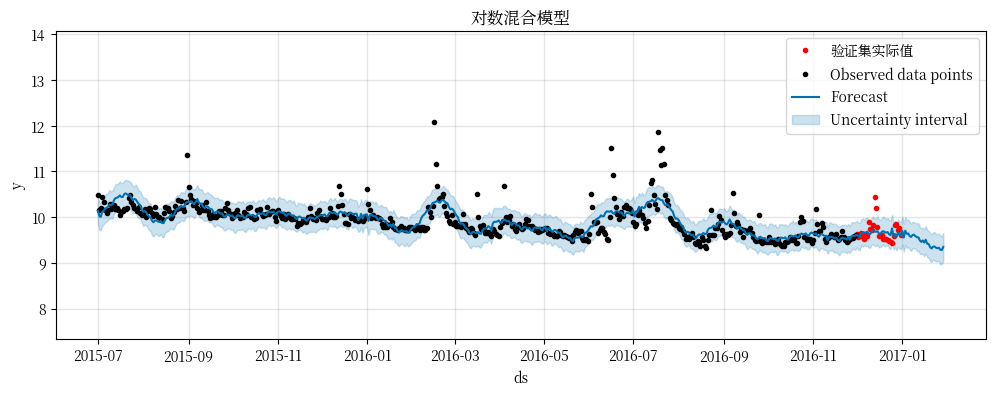
\includegraphics[width=\linewidth]{figures/prophet_mix.png}
  \caption{Prophet 混合模型}
\end{subfigure}
\caption{Prophet 几个模型的结果}
\label{compare_model}
\end{figure}

图\ref{compare_model}中,使用普通模型的 SMAPE 的分数为 0.25758,使用假日模型的 SMAPE 的分数为 0.22900,使用混合模型的 SMAPE 的分数 0.14071。SMAPE 的分数越低,代表着模型的预测性能越好。
三个图片中,小红点是验证集的实际值,小黑点显示训练集的实际值,蓝色的线代表着prophet模型的预测值,蓝色的区域是置信区间,上面是可能区间上限,下面是可能区间下限。
可以很直观的看到,仍旧存在某些没有预测到的特殊因素,需要额外的参数输入。
经过查询与泰勒·斯威夫特的新闻有很大关系。总的来说虽然蓝色的线并没有覆盖掉全部的训练集数据,但是在其他的条件下,基本有效的预测了访问量数据。
考虑了周期性和假日性的 prophet 还是没有达到最好的效果,不过勉强也可以了。

\section{两种算法的比较以及选择}

通过 SMAPE(对称平均绝对百分比误差)的比较,得到了了两个模型根据相同数据下最好的参数下的表现。但是仅仅是针对这一条数据下的表现,不具有普遍性,所以需要对每一个词条都要做拟合并预测得到每一个词条的 SAMPE 分数。
最后比较最后的平均值即可。结果如下图\ref{compare_model2}所示。

\begin{figure}[htbp]
  \centering
  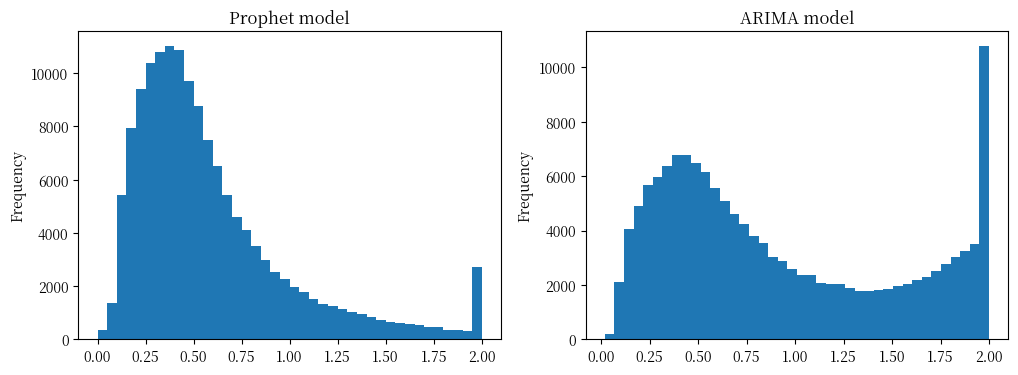
\includegraphics[width=\textwidth]{validation_compare.png}
  \caption{模型 SMAPE 分数的比较}
  \label{compare_model2}
\end{figure}

很直观的看到了两个模型的性能,prophet 的最后 SAMPE 得分为 $0.586509$,ARIMA 的最后得分为 $0.919387$。
虽然在某些个词条例如泰勒斯威夫特下表现和 prophet 的模型没有太大差异,但是没有经过一个一个对词条的参数的调整(笔者最后使用 auto\_arima 自动选择合适的词条参数),拟合结果就不尽人意,ARIMA 的预测准确度会大大下跌。
所以最后选择了考虑了周期性(季节性)、假日性、特殊因素、趋势项的 prophet 模型。

\section{本章小结}

在本章节首先介绍了数据的来源以及数据的特点,并对预测词条的时间序列做了处理。然后探讨当前常见的时间序列预测算法,决定使用 ARIMA 和近年来比较先进的 prophet 算法进行实验和探究。最后比较两个算法对所有词条的分数的平均值,结果表明prophet算法有更好的预测效果。

%%================================================
%% Filename: chap04.tex
%% Encoding: UTF-8
%% Author: 苏峻锋
%%================================================
\chapter{基于时间卷积网络的剩余性能的预测}
服务器集群运行时,由于访问时间,访问任务的不同,某些时间段整个集群可能处于忙碌的状态,某些节点可能处于任务繁忙任务重的而其他节点空闲的问题。
这样的两种节点是两种状态,高负载状态和低负载状态,处于低(高)负载状态的需要通过负载均衡器调整为正常负载状态,可以提高集群的总体资源利用率,环节高负 载节点的压力。
因此本章通过对于时间卷积网络的研究,针对某一个节点的剩余性能的预测,使得对服务器节点的负载分配进行均衡的调整。本文通过对普遍的 Linux 进行研究来获取相关数据。
\section{服务器剩余性能的获取}
动态负载均衡算法的负载性能会受到服务器负载指标选取的影响。选择合适的负载信息生成合适的负载指标能够真实的反映服务器运行是的负载情况,
提升算法的准确度和动态负载均衡的负载效果。在第二章中已经知道了有哪些负载信息值得挑选和收集,但是没有一个真正的合适的负载综合指标来体现真实的负载情况。
具体的剩余性能的获取可以使用 Linux 的 proc 文件系统获取,该文件储存在内存里,不会占用外存的空间。

(1)CPU 信息的获取 

要获取 Linux 系统中的 CPU 详细使用情况可以使用 cat/proc/stat,CPU 详细使用情况如下表。

\begin{longtblr}[
  caption = {CPU 详细信息解释},
]{
  width = \linewidth,
  colspec = {Q[102]Q[837]},
  vline{2} = {-}{},
  hline{1,9} = {-}{0.08em},
  hline{2} = {-}{},
}
参数      & 解释                                   \\
user    & 系统从启动到当前时刻,用户态 CPU 时间,不含 nice 值为负的进程 \\
nice    & 系统从启动到当前时刻,nice 值为负的进程占用的 CPU 时间     \\
system  & 系统从启动到当前时刻,核心时间                      \\
idle    & 系统从启动到当前时刻,除硬盘等待外其他等待时间              \\
iowait  & 系统从启动到当前时刻,硬盘等待时间                    \\
irq     & 系统从启动到当前时刻,硬中断时间                     \\
softirq & 系统从启动到当前时刻,软中断时间                     
\end{longtblr}

那么 CPU 利用率的计算公式为:$CPU_{usg} = 1 - (idle_2 - idle_1) / (cpu_2 - cpu_1)$ 通过使用 cat /proc/cpuinfo 命令获取服务器 CPU 配置,然后在 benchmark 上可纯到该 CPU 性能的分数作为 $CPU_{mark}$。则一个节点的 CPU 的剩余性能如下。
\begin{align}
  C_{j}=(1-CPU_{usg_{j}})\frac{n^{\ast}CPU_{mark_{j}}}{\sum_{1}^{n}CPU_{mark}}
\end{align}

(2) 内存信息获取
获取内存使用情况则可以 cat /proc/meminfo 命令,其中最重要的是 MemFree、Buffers、Cached 三个信息分别是完全空闲的内存大小、缓存文件系统的元数据和跟踪正在读写的块设备、存储页缓存和slabs的内存大小。所以内存使用率的计算方式如下。
\begin{equation}
  MEM_{usg} = (1 - MemFree + Buffers + Cached) / MemFree
\end{equation}

(3)磁盘信息获取

磁盘信息可以通过 iostat -x /dev/sda1  命令获取。重要信息如下表。

% \usepackage{tabularray}
\begin{longtblr}[
  caption = {磁盘信息获取},
]{
  width = \linewidth,
  colspec = {Q[81]Q[860]},
  hlines,
  vlines,
  hline{1,8} = {-}{0.08em},
}
标示~     & 说明                                                 \\
Device~ & 监测设备名称                                             \\
rkB/s~  & 每秒实际读取的大小,单位为KB                                    \\
wkB/s~  & 每秒实际写入的大小,单位为KB                                    \\
await~  & 等待I/O平均的时间(milliseconds)                           \\
svctm~  & I/O需求完成的平均时间                                       \\
\%util~ & 设备带宽的使用率,达到100\%表示饱和,达到性能瓶颈,如果是支持处理并发请求的设备则不代表性能瓶颈 
\end{longtblr}

(4)网络带宽信息获取

获取网络带宽使用 cat /proc/net/dev 命令,统计一段时间内 Receive 和 Tramsmit 的 bytes 值变化,可以获取网口传输速率 $T_{bytes}$,而网络带宽为 Bandwidth,则带宽利用率为:$NET_{usg} = T_{bytes} / Bandwidth$

获取了这几个重要的剩余性能的指标之后,也需要有一个能够体现综合负载情况的评价指标。为了以一种数学方法客观的计算出服务器节点当前的负载量,需要改造一个综合负载决策来组合各项负载指标。
常见的指标组合形式有加权和法和加权乘法,通过阅读不同的文献可知,在构建服务器负载状态的数学模型中,加权和法具有不错的效果\cite{lixbhunj}。在以往的负载均衡策略研究中这些权重系数通常依靠经验赋值确定,缺乏必要的数学分析和定量依据,为了使得服务器的计算结果更加准确和可靠,本文选取了主成分分析法科学计算综合负载决策函数的权系数向量。

主成分分析法(Principal Componet Analysis, PCA)最早是由 Pearson\cite{kpfrs1901lines}提出的一种多元统计方法,
该方法通过正交变换将原始数据转换成一组由线性无关变量变量表示的数据,以达到数据降维的目的\cite{李可佳2023基于主成分分析和函数机制的差分隐私线性回归算法}。具体步骤如下。

已经收集了服务器节点的 CPU 利用率、内存利用率、设备 IO 使用率,和带宽使用率的数据,将这些数据保存在以个表中,每一列代表一个指标,每一行代表一个观测时间点的数据。
由于主成分分析法的要求,将不同的特征量纲统一到相同的尺度,这样就可以公平地比较和组合这些特征,需要对给定数据集进行标准化。
对于每个指标,计算所有数据点的均值。公式为:$\mu=\frac{1}{N}\sum_{i=1}^{N}x_{i}$ 其中$\mu$ 为均值,N 是观测的个数,$x_{i}$ 每个观测的值。
计算标准差:然后计算每个指标的标准差。公式为:$\sigma = \sqrt{\frac{1}{N} \sum_{i = 1}^{N} \left(\right. x_{i} - \mu \left(\left.\right)\right)^{2}\frac{\sigma}{2}}$其中$\sigma$是标准差。
最后进行Z-score标准化:对每个指标的每个数据点进行标准化,公式为 $z = \frac{(x_{i} - \mu)}{\sigma}$ 其中 $z$ 就是最后每个指标每个观测时间的标准化后的值。

给定标准化后的数据集 $X = [x_1, x_2, \cdots, x_n]^{\mathbf{T}} \in \mathbb{R}^{n \times d}$,其中 $n$ 为样本的数量,$d$ 指标的数量,
结合在一起,\( X \) 是一个由 \( n \) 个 \( d \)-维的实数向量构成的数据集,并且以矩阵形式表示,其中每一行是一个样本,每一列是一个特征。则数据集的协方差公式矩阵如下。
\begin{equation}
  A={\frac{1}{n}}X^{\mathsf{T}}X={\frac{1}{n}}\sum_{i\,=\,1}^{n}x_{i}x_{i}^{\mathsf{T}}=V\Sigma V^{\mathsf{T}}\in\mathbb{R}^{d\cdot d}
\end{equation}

对 $\mathbf{A}$ 进行特征分解后得到一组降序排列的特征值$\lambda_1 \ge \lambda_2 ... \ge \lambda_n > 0$ 相对应的单位特征向量 $v_1, v_2, \dots, v_n$。
其中,特征值越大的,其对应的主成分越重要。于是,综合负载决策函数如下。
\begin{equation}
  \mathbf{X} = \mu_1C_{usg} + \mu_2M_{usg} + \mu_3D_{usg} + \mu_4N_{usg}
\end{equation}

通过指定欲保留的主成分比重阈值 $\theta \in (0, 1]$ 来确定目标唯独 k 的大小。
具TCN 模型参数组合体来说$\k$可以通过 $\frac{\sum^{k}_{i = 1}\lambda_i}{\sum^{d}_{i = 1}\lambda_i} \ge \theta$ 来得到。
取前 $k$ 个特征值对应的特征向量组成的主成分空间$\mathbb{V}_{d \times k} = (v_1, v_2, \cdots, v_k)$。将标准化后的原始数据集$\mathbf{X}_{n \times d}$ 投影到由前 $k$ 个特征向量构成的主成分空间 $\mathbf{V}_{d \times k}$中,得到了降维后的 $k$ 维数据集。
\begin{equation}
  \mathbf{Z}_{n \times k} = \mathbf{X}_{n \times d}\mathbf{V}_{d \times k}
\end{equation}

在这个公式中,$\mathbf{X}_{n \times d}$ 表示标准化后的原始数据集,其中 $n$ 是样本数,$d$ 是原始特征数。$\mathbf{V}_{d \times k}$ 包括了前 $k$ 个特征值对应的特征向量(这些特征向量通常是按照特征值大小从大到小排列的),它们构成了主成分空间。这个空间的维度($k$)通常远小于原始特征空间的维度($d$)。

当原始数据集 $\mathbf{X}$ 与主成分空间 $\mathbf{V}_{d \times k}$ 相乘时,得到的 $\mathbf{Z}_{n \times k}$ 就是投影到这个 $k$ 维空间的数据集。在这个 $k$ 维空间中,每一行代表了原始数据的一个样本,每一列则对应一个主成分。$\mathbf{Z}$ 的列向量提供了在主成分空间中的坐标,即降维后的数据表示。

其中在进行特征分解后,就已经得到了主成分空间,空间内含有了最重要的4个特征值,
这个特征值就是权重的系数,通过降维与原始数据值相乘后得到的就是每个指标乘以权重系数后的数据集,只需要对降维的数据集进行每一列的相加,即可对得到时间序列-综合负载指标的数据集。

\section{时间卷积网络的关键特征}
时间卷积网络由传统的 CNN 改进的专门处理时间序列的深度学习模型\cite{lea2016temporal}。一开始认为,时序问题(如语言、语音等等)天生就是 RNN 的地盘。然而现在这一观点要成为过去式了。时间卷积网络(Temporal Convolutional Nets, TCNs)作为 CNN 家族中的一员健将,拥有许多新特性,如今已经在诸多主要应用领域中击败了 RNN。看起来 RNN 可能要成为历史了。

卷积神经网络(Convolutional Neural Nets, CNNs)是图像和视频识别领域公认的主力军,
而循环神经网络(Recurrent Neural Nets, RNNs)在自然语言处理领域的地位与其是相似的。
但二者的一个主要不同是,CNN 可以识别静态图像(或以帧分割的视频)中的特征,
而 RNN 在文本和语音方面表现出色,因为这类问题属于序列或时间依赖问题。
也就是说,待预测的后一个字符或单词依赖于前面的(从左到右)字符或单词,因此引入时间的概念,
进而考虑到序列。实际上,RNN 在所有的序列问题上都有良好表现,包括语音 / 文本识别、机器翻译、手写体识别、序列数据分析(预测),
甚至不同配置下的自动编码生成等等。但是它的问题是极度地计算密集,因为在整个任务运行完成之前,必须保存所有的中间结果,深度神经网络必须等前一个单词处理完,才能进行下一个单词的处理,于是 TCN 便应运而生。

时间卷积网络需要的数据集和RNN 有一定的类似,在处理时间序列数据集时都要进行嵌入(Embedding)操作。Embedding的主要目的是将时序数据映射到一个稠密的连续向量空间中,使得相似的语义信息在该向量空间中也能够彼此接近。这样,神经网络就可以基于这些向量表示学习到输入数据的复杂语义信息,并在相似的向量表示之间进行泛化。图是具体的嵌入过程。

\begin{figure}[htbp]
  \centering
  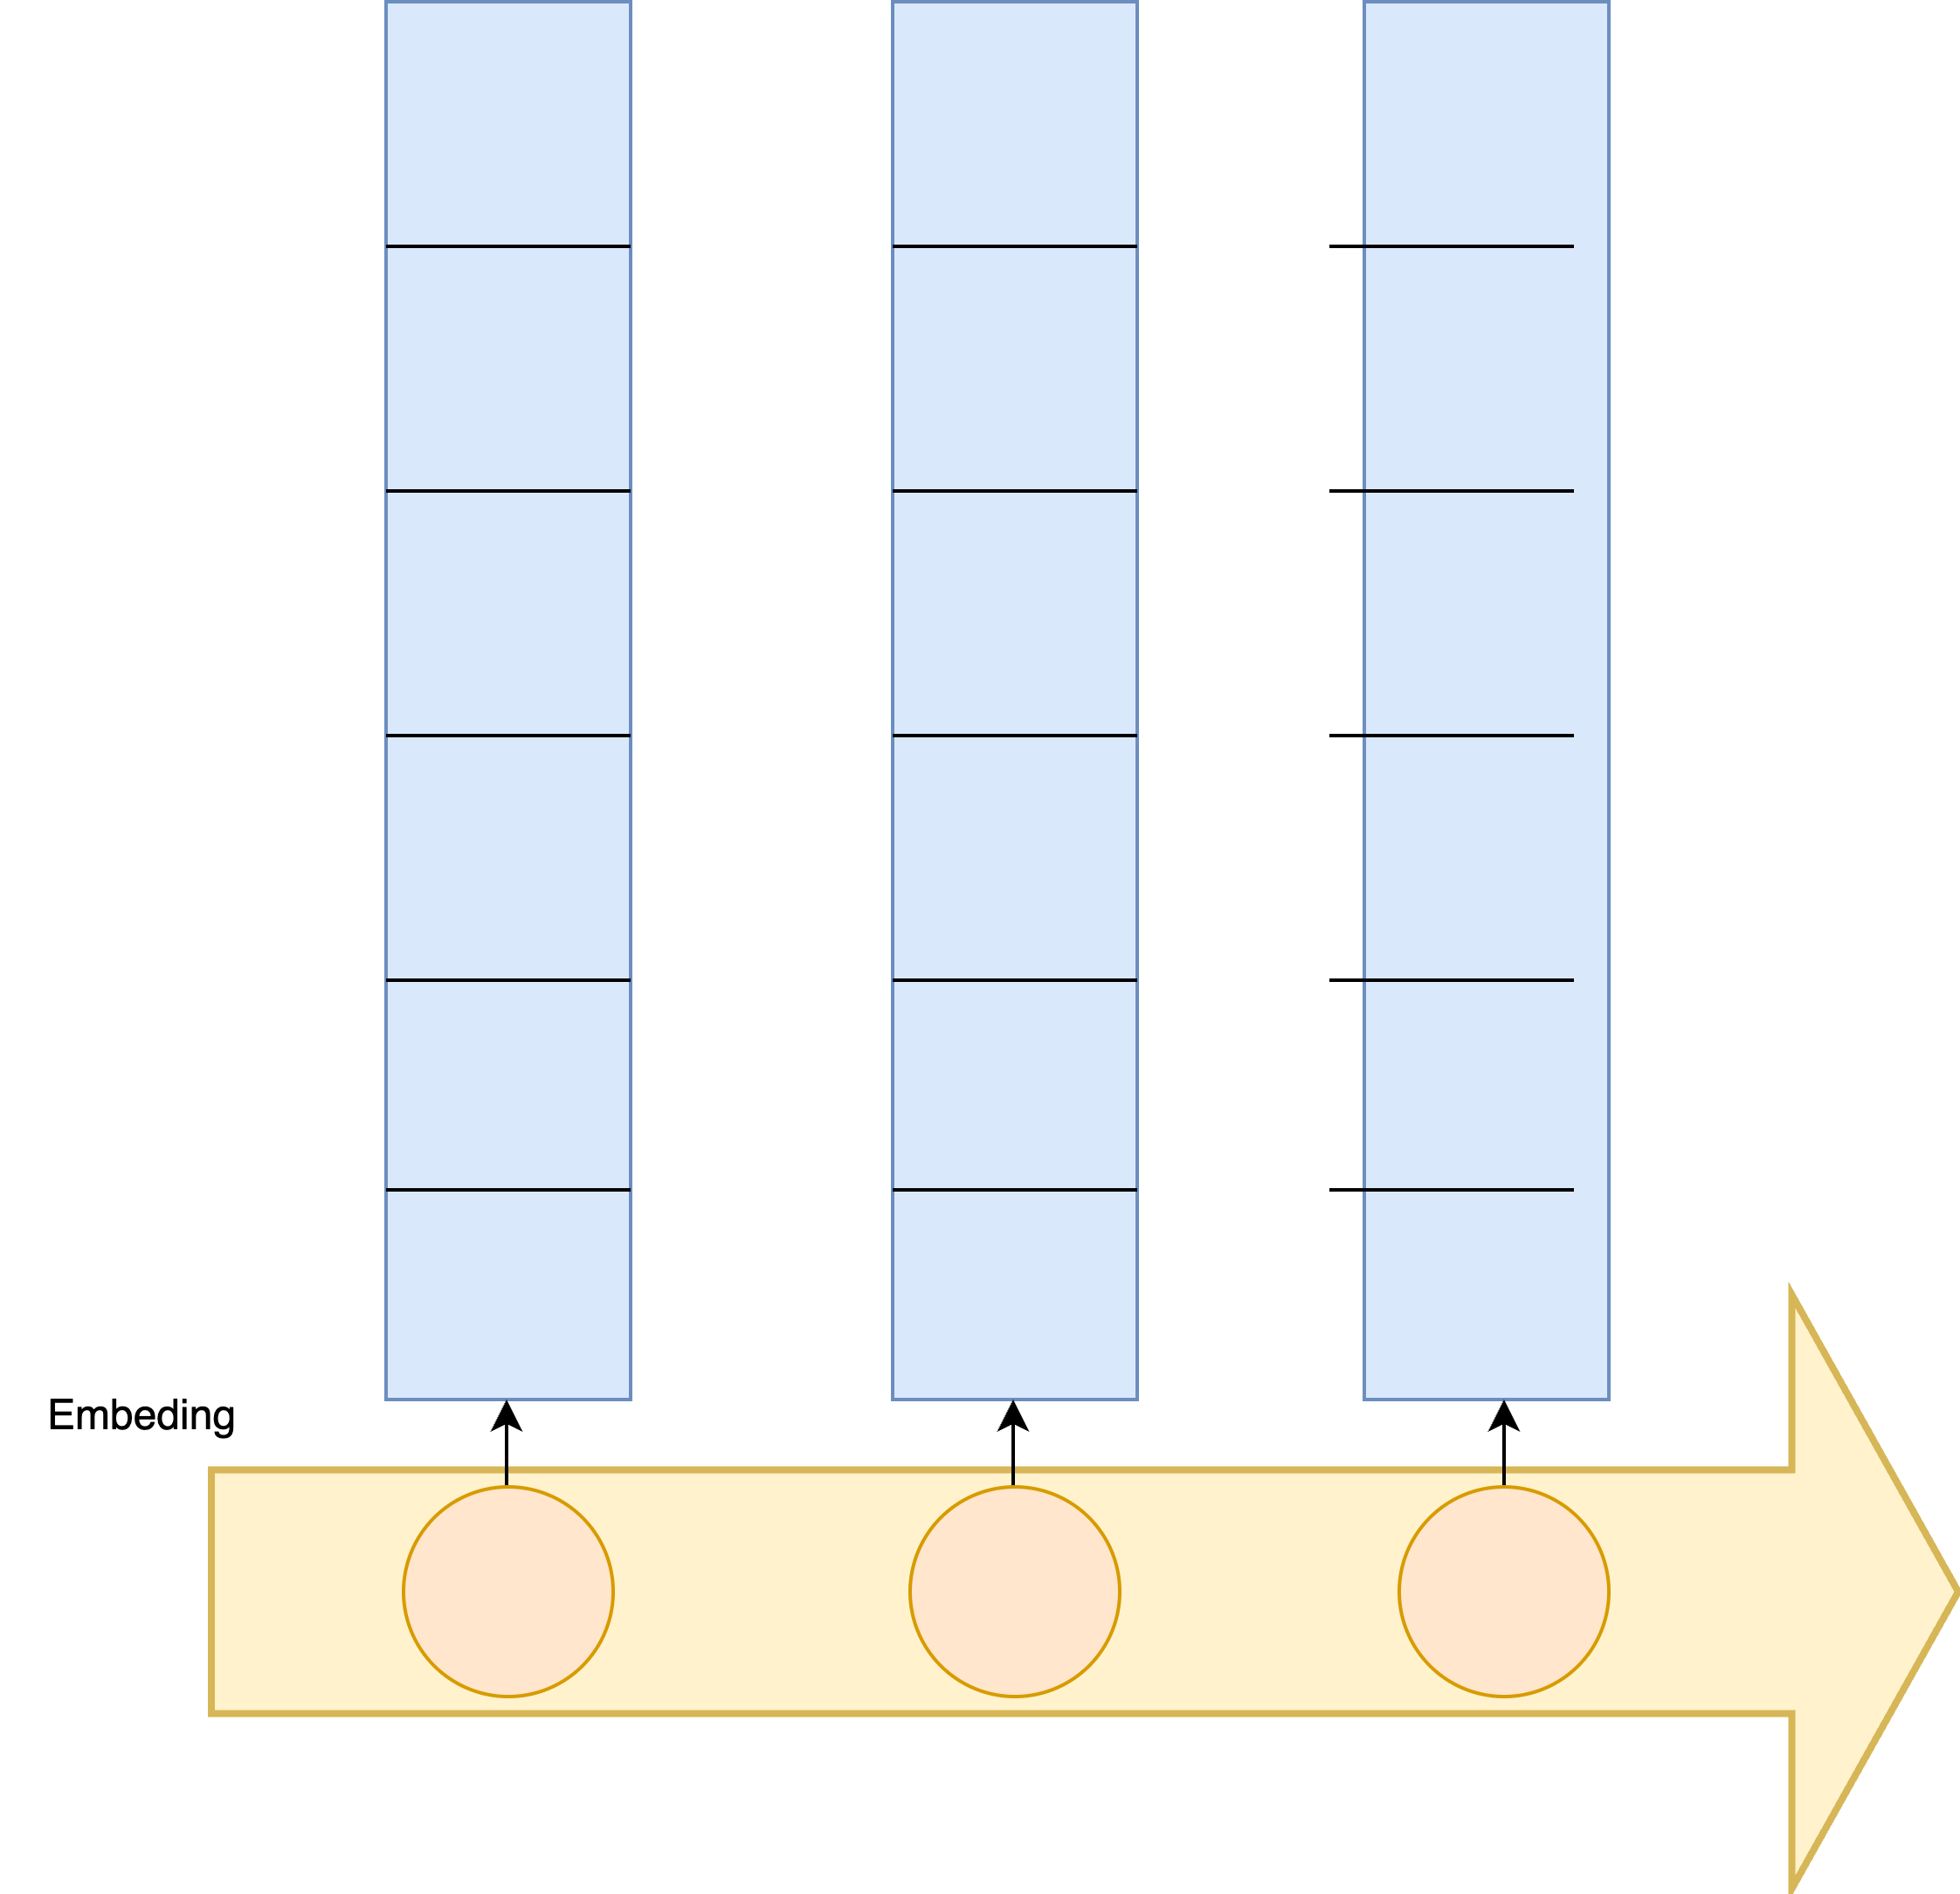
\includegraphics[width=0.7\textwidth]{figures/embedding.png}
  \caption{原始时序序列嵌入生成向量}
\end{figure}

TCN所依赖的卷积操作在本质上就是一维卷积(1D-CNN)。一维卷积利用多个大小固定的卷积核与输入序列进行卷积运算来生成输出序列。卷积核的形状由输入通道数$in\_channels$ 和卷积核大小$kernel\_size$ 共同决定,卷积核的数量则由输出通道数$out\_channels$决定。
经过Embedding后的时序数据的通道数由1扩展成了$embedding\_size$ ,对于有着 $in\_channels$ 个通道的时序数据作为输入, 一维卷积使用 $out\_channels$ 个大小为($in\_channels, kernel\_size$)的卷积核进行卷积操作。

假设有一个时间序列,总共有五个时间点,比方说股市,有一个股票的价格波动:[10,13,12,14,15]。TCN 使用一个卷积大小为 2 的卷积核,对上面5个数据做一个卷积核大小为2的卷积是什么样子如下。

\begin{figure}[htbp]
  \centering
  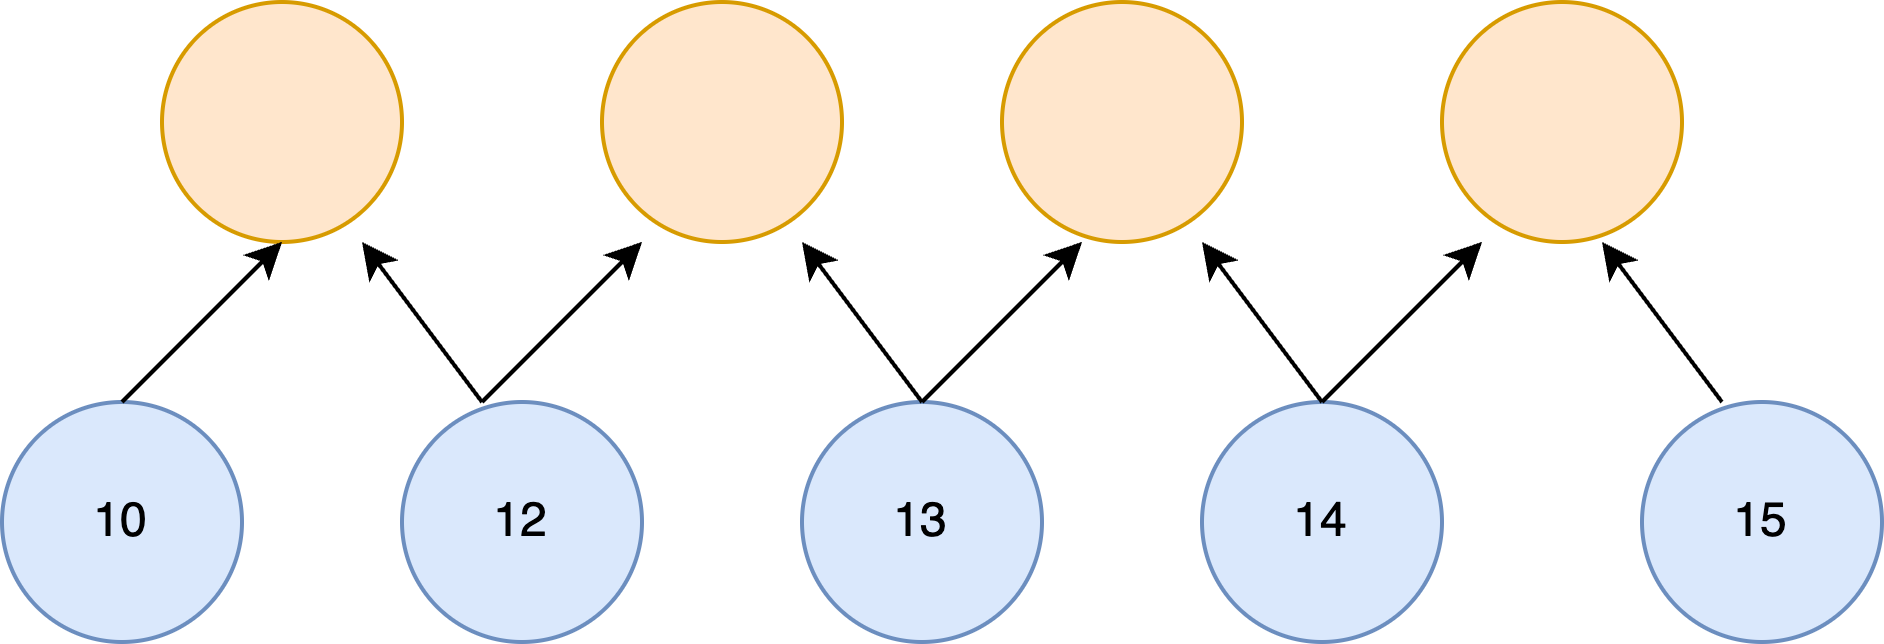
\includegraphics[width=.9\textwidth]{figures/convolution_1.png}
  \caption{卷积核为2的卷积过程}
\end{figure}

五个数据经过一次卷积,可以变成四个数据,
但是每一个卷积后的数据都是基于两个原始数据得到的,所以说,目前卷积的视野域是2。可以看到是输入是5个数据,但是经过卷积,变成4个数据了。TCN网络的第一个原则是输入和输出的形状必须相同。而在进行一维卷积操作时,假设第$i$ 层的输入长度为$L_i$ 卷积核大小为 $K$ 则输出长度为 $L_{i+1} = L_{i} - K + 1$。为满足这个原则,TCN在使用卷积神经网络进行序列处理时,通常需要进行 Padding 操作。通过在输入序列的左侧添加一定数量$K-1$ 的 0,实现信号维度的保持,使通过卷积和池化处理后的数据与输入数据的长度相同。在一维卷积中进行的Padding操作默认会在左右都进行填充,
所以TCN进行了额外的裁剪操作。

\begin{figure}[htbp]
  \centering
  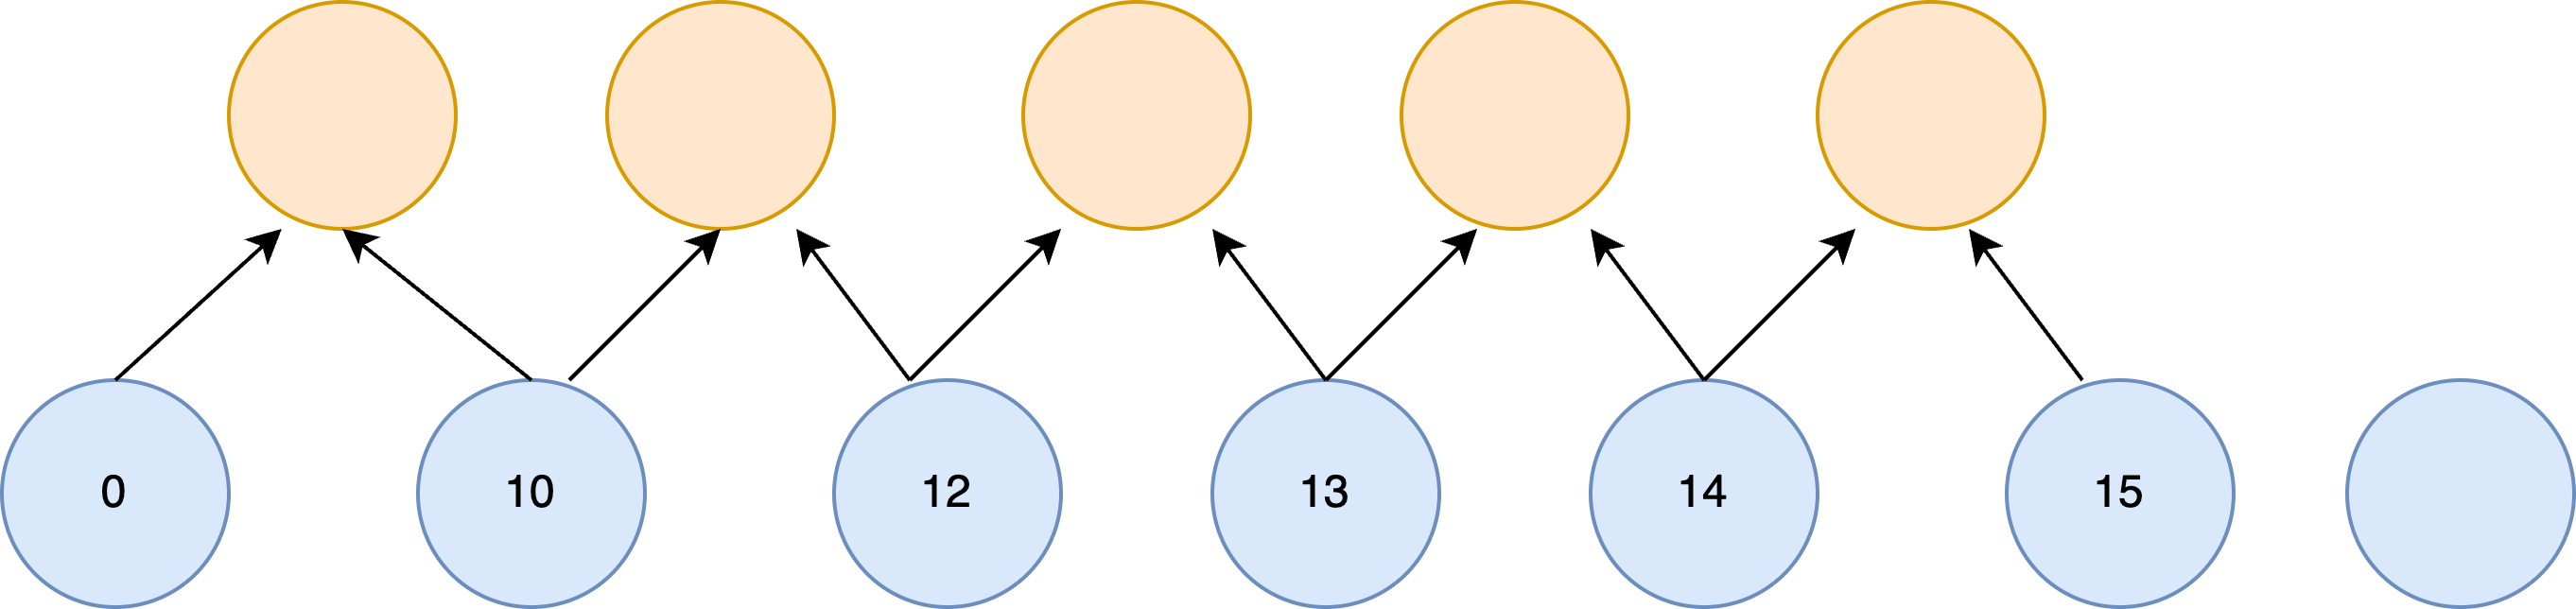
\includegraphics[width=0.9\textwidth]{figures/convolution_2.png}
  \caption{padding 后的卷积}
\end{figure}

padding是左右两头都增加0,如果padding是1的话,就是上图的效果,其实会产生6个新数据,但是秉着:“输入输出尺寸相同”和“我们不能知道未来的数据”,所以最后边那个未来的padding,就省略掉了,之后会在代码中会体现出来。

时间卷积网络有两个原则,其一就是上面的TCN 网络的输入和输出形状必须相同,以确保模型对时序数据的处理不会丢失信息。其二,TCN 网络中的每一时刻的输出仅由该时刻及其之前的输入卷积得到,以确保其在处理序列时具有因果约束。
通过使用因果卷积满足原则二,因果卷积是一种只考虑过去时间状态的一维卷积操作。因果卷积的具体步骤如下图所示。

\begin{figure}[htbp]
  \centering
  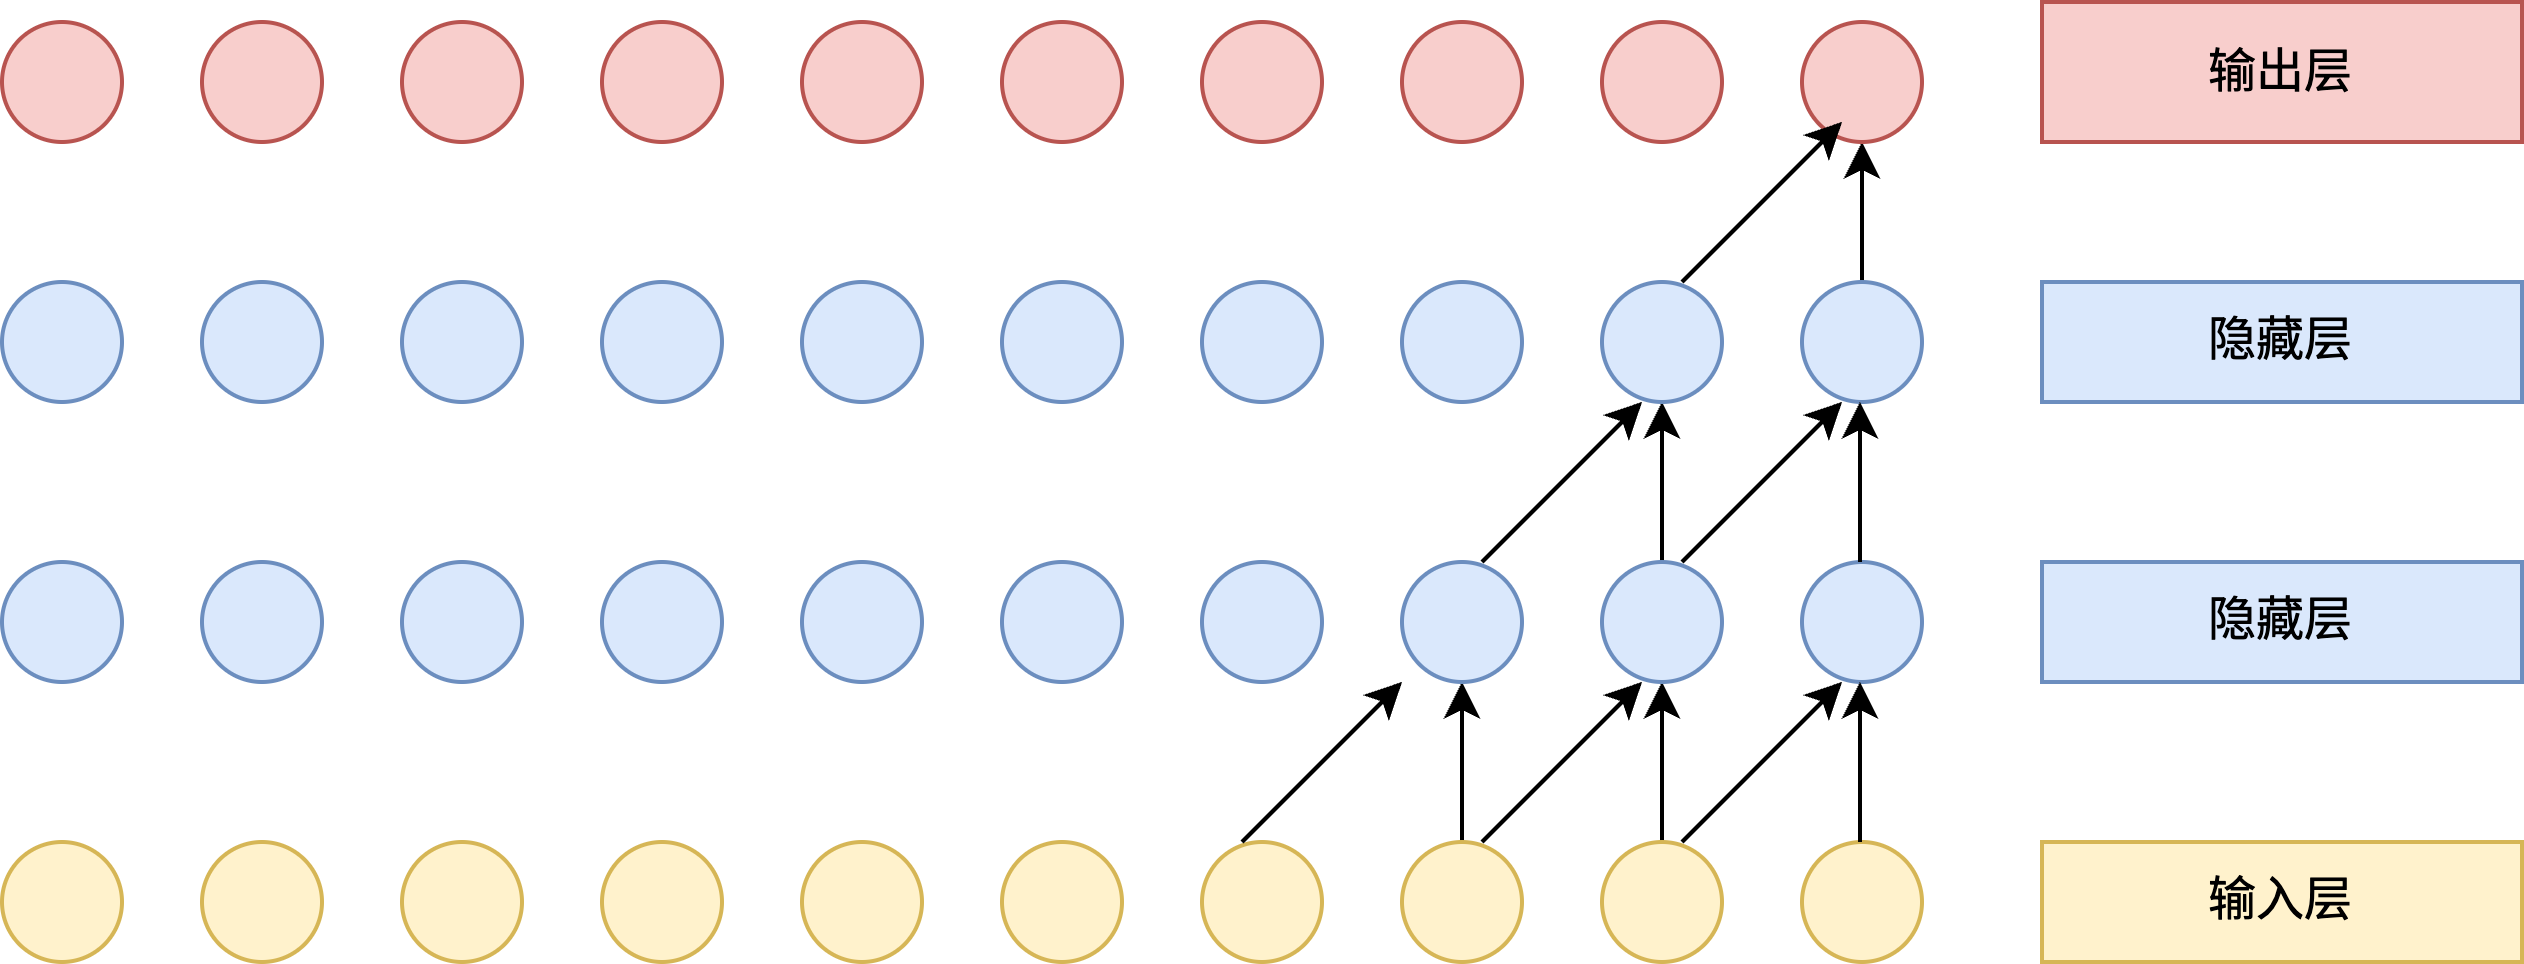
\includegraphics[width=\textwidth]{figures/causal_convolution.png}
  \caption{因果卷积}
\end{figure}

图中可以看到,因果卷积具备了两个特点。只考虑过去的信息。 时刻的输出$y_t$ 仅依赖于 $x_0,...,x_t$ ,而不依赖任何“未来”的输入$x_{t+1},...,x_T$。
同时追溯历史信息越久远,隐藏层越多。 图中,输出层期望采集输入层的4个时间步,则需要2个隐藏层。而业务的需求往往要求采取更多的时间步,确实是“深度”学习了。

由于因果卷积没有循环连接,它们通常比循环神经网络(RNN)训练速度更快,尤其是应用于非常长的序列。
但是,针对于一般的时间序列而言,往往是按照分钟记录的,那少说也是十万、百万的数据量,想要考虑之前1000个时间点呢?视野域要是1000,那意味着要999层卷积。
每经过一层,节点相对于前层减少一个,我们最后的输出只有一个节点,如果输入视野为1000,需要经过999层才能变为最后输出的一个节点。
啥计算机吃得消这样的计算。所以引入了膨胀因果卷积。

单纯的因果卷积还是存在传统卷积神经网络的问题,即对时间的建模长度是受限于卷积核大小的,如果要想抓去更长的依赖关系,就需要线性的堆叠很多的层。
标准的 CNN 可以通过增加 pooling 层来获得更大的感受野,而经过 pooling 层后肯定存在信息损失的问题。

膨胀卷积是在标准的卷积里注入空洞,以此来增加感受野。
和传统卷积不同的是,膨胀卷积允许卷积时的输入存在间隔采样,采样率受超参数 dilation rate控制,
指的是做卷积操作时kernel里面的元素之间的下标间隔。空洞的好处是不做 pooling 损失信息的情况下,增加了感受野,让每个卷积输出都包含较大范围的信息。下图就是 dilation=2 的时候的膨胀因果卷积的情况,

\begin{figure}[htbp]
  \centering
  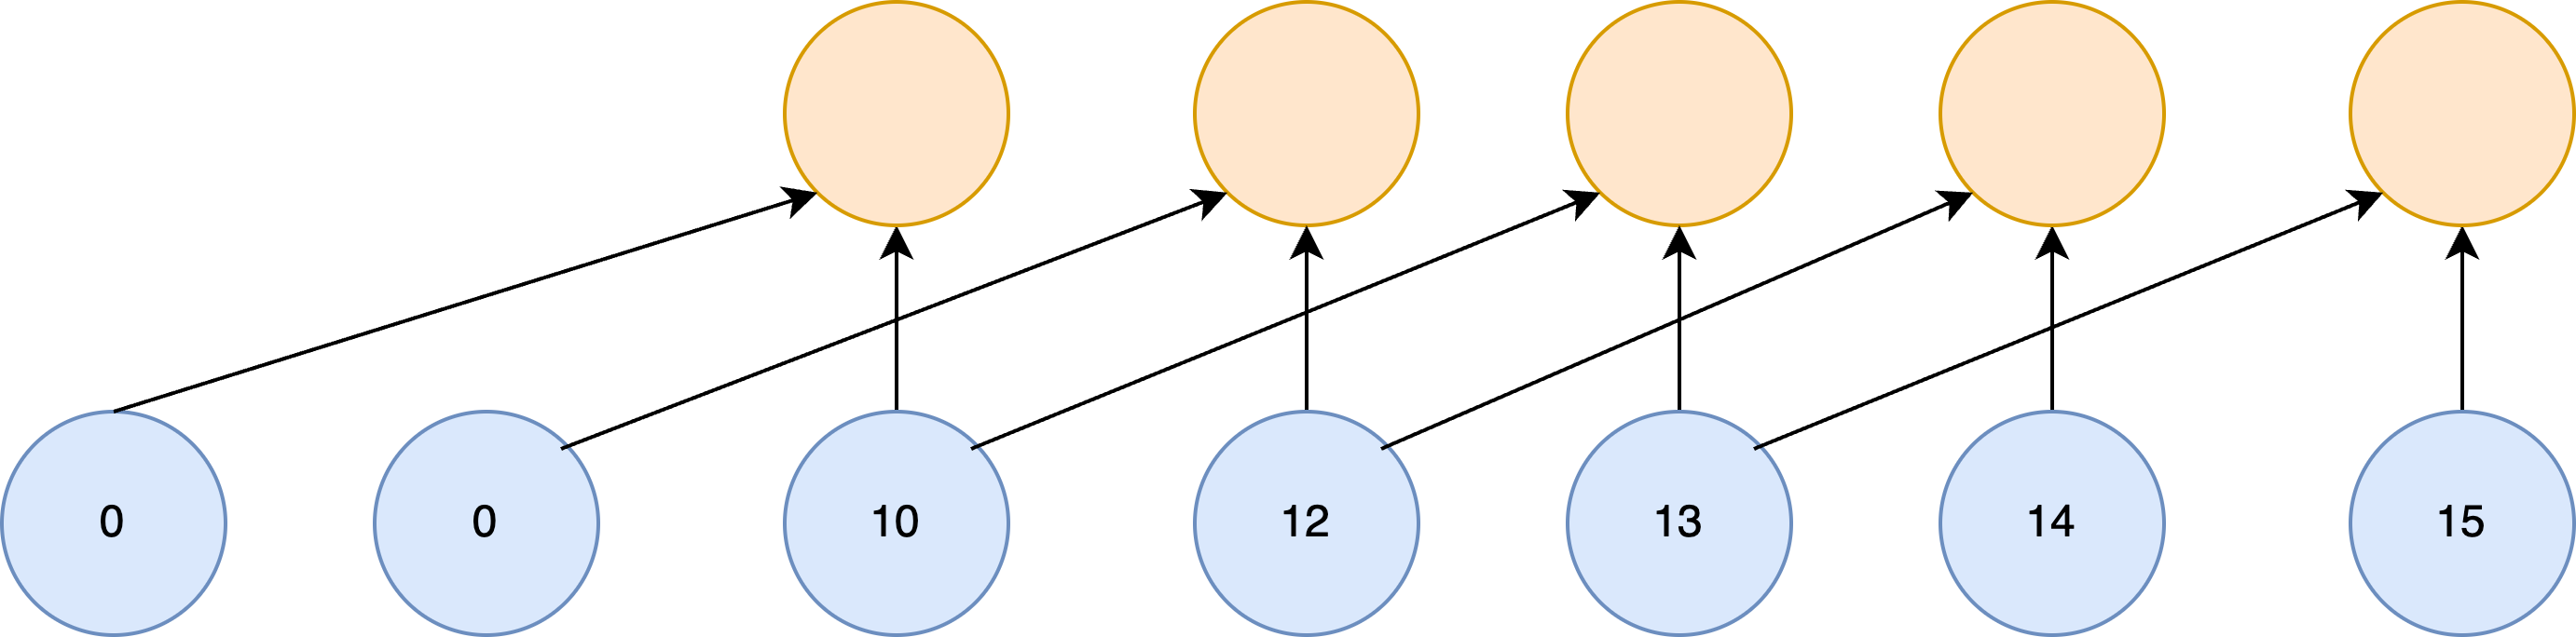
\includegraphics[width=\textwidth]{figures/dilation_convolution.png}
  \caption{dilation=1 的膨胀因果卷积}
\end{figure}

图中,可以看到卷积核大小依然是2,但是卷积核之间变得空洞了,每2个点采样一个作为输入;
如果dilation=3的话,那么可以想而知,这个卷积核中间会空的更大,每3个点采样一个作为输入。
因为dilation变大了,所以相应的padding的数量从1变成了2,所以为了保证输入输出的特征维度相同,
padding的数值在卷积核是2的情况下等于dalition的数值。
一般情况下,$padding=(kernel_size-1)\times dilation$,每个卷积核元素之间有 $dilation - 1$ 个空洞节点,
所以空洞因果卷积的感受野范围大小为 $(kernel_size-1) \times dilation + 1$。
以输入中的第一个元素作为空洞因果卷积的最后一个元素,则它的左边需要padding的个数为$(kernel_size-1) \times dilation$。于是较为完备的 TCN 训练网络如下。

\begin{figure}[htbp]
  \centering
  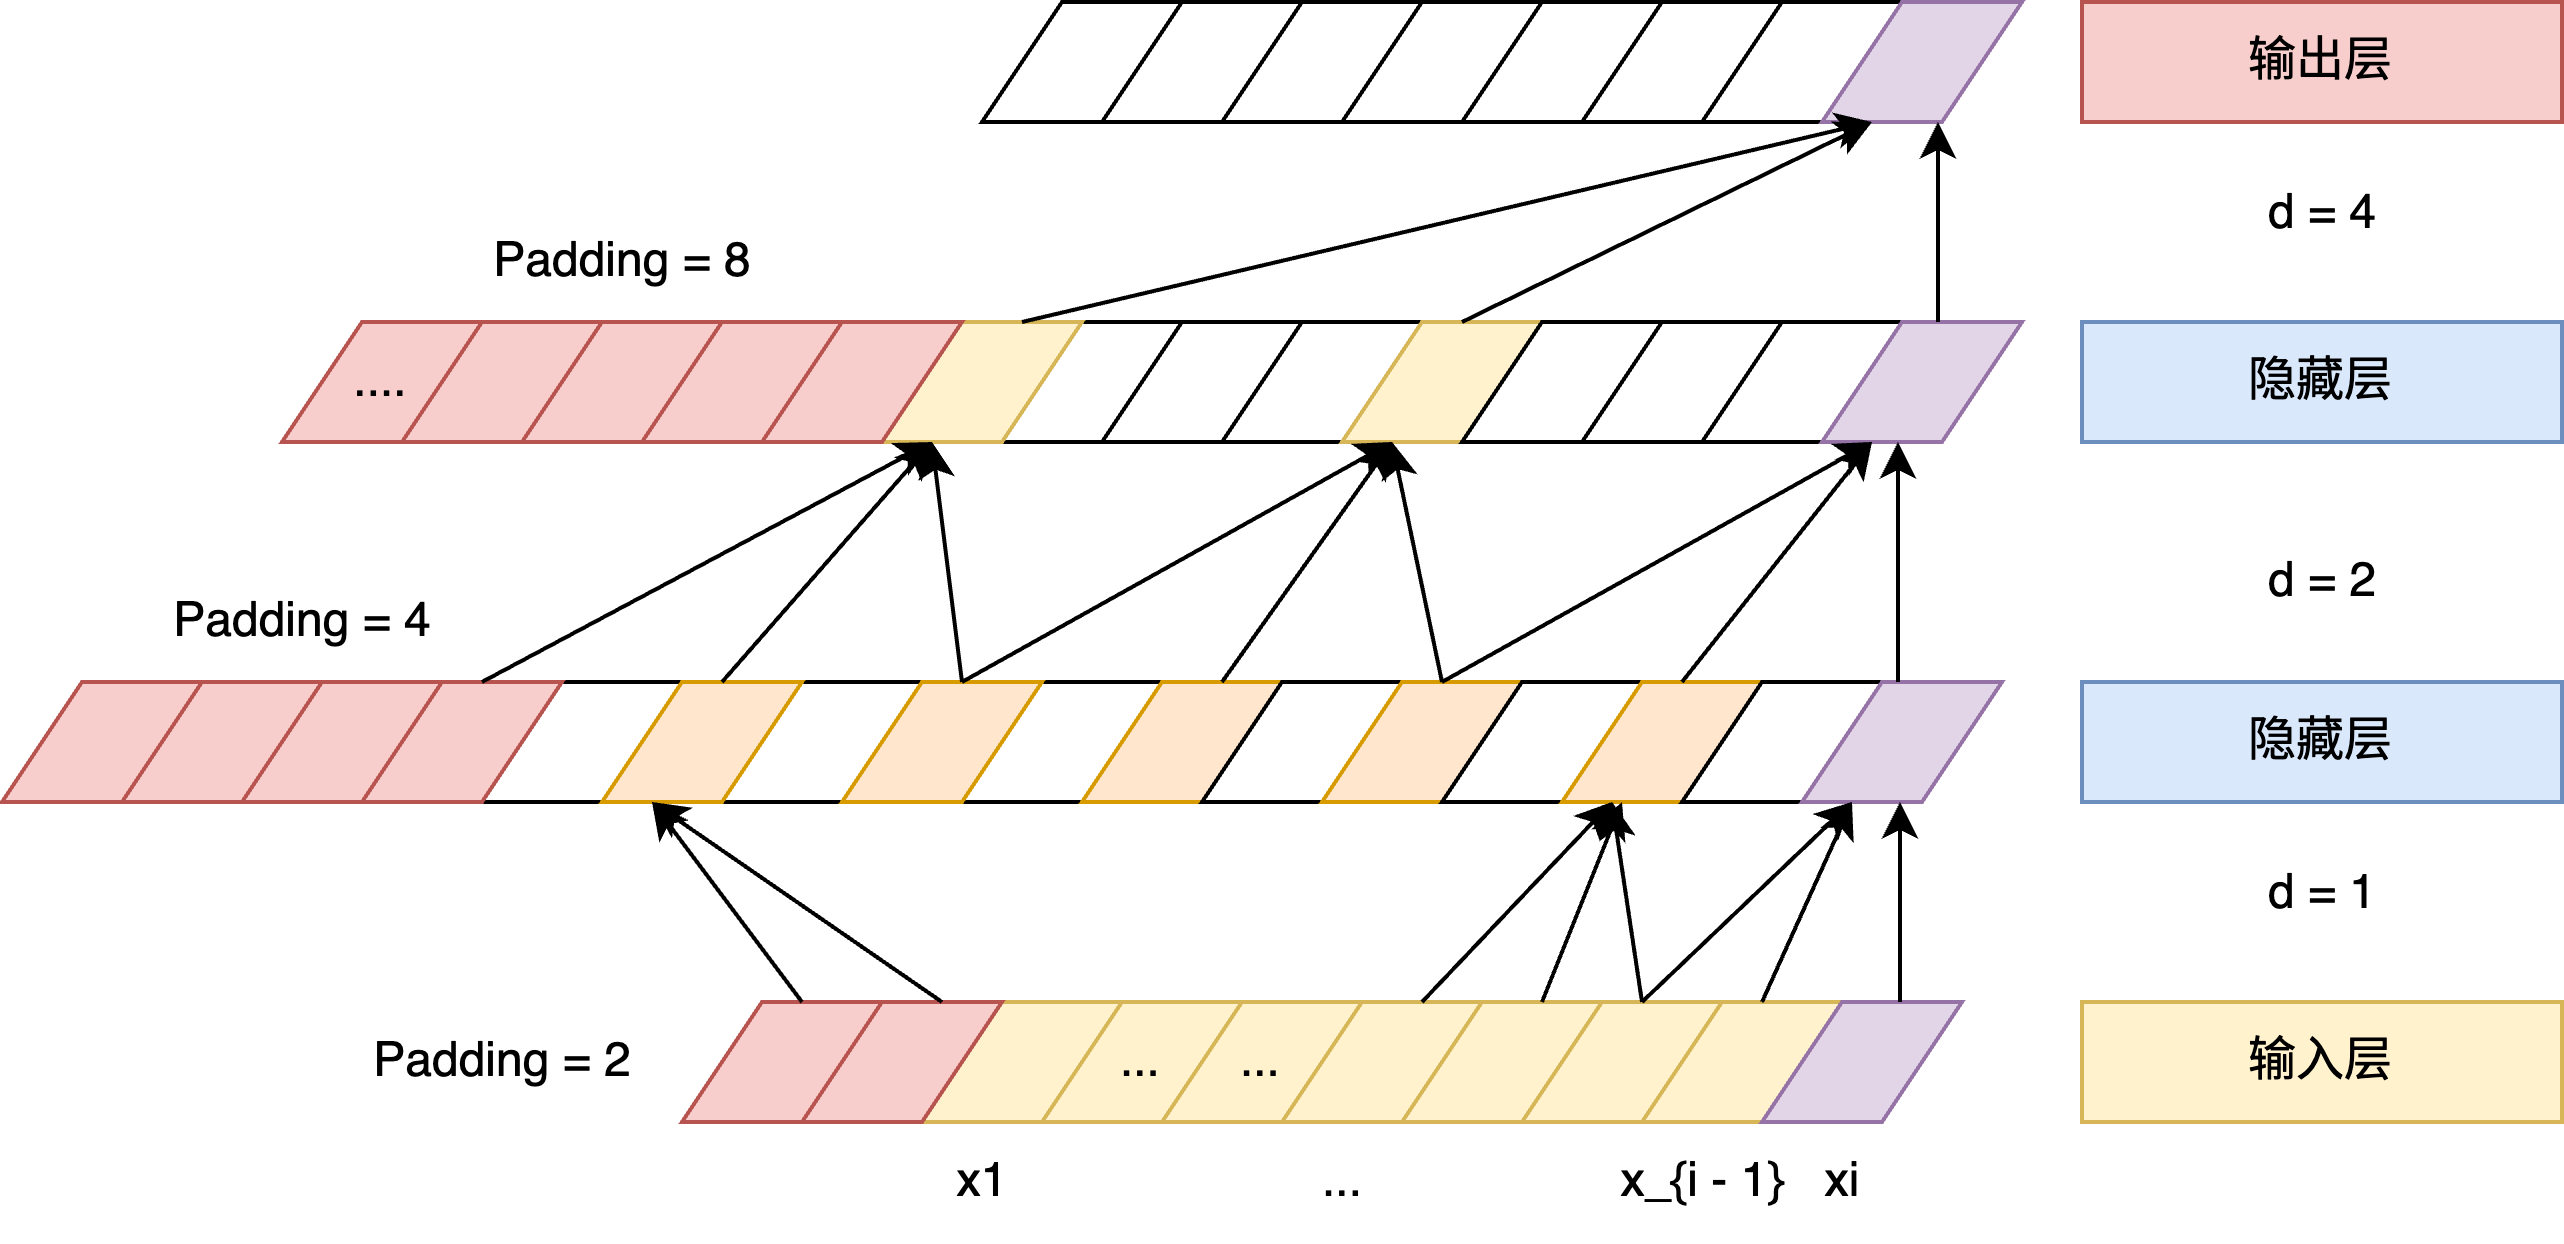
\includegraphics[width=\textwidth]{figures/tcn_1.png}
  \caption{TCN 训练网络骨干}
\end{figure}

从图中可以看到,每一层$t$ 时刻的值只依赖于上一层 $t, t - 1, \dots$ 时刻的值,体现了因果卷积的原则。而每一层对上一层信息的提取,都是跳跃式的,且逐层 dilated rate 以 2 的指数增长,体现了空洞卷积的特性。同时由于采用了空洞卷积,因此每一个隐藏层都需要做 padding,padding 的大小为 $padding = (kernel_size - 1)$。

在 CNN 中能够提取不同的特征,网络层数越多,意味着能够提取到不同等级的特征,并且,越深的网络提取的特征越抽象,越具有深层次的信息。但是如果简单的增加深度,就会导致梯度消失或者梯度爆炸。对于这个问题可以使用权重参数初始化和正则化层,这样可以训练几十层的网络\cite{吕国豪2014基于卷积神经网络的正则化方法}。
虽然解决了梯度消失的问题,但是网络退化出现了。高层次的神经网络空间虽然包含了低层次的网络空间,但是由于在训练中使用的是随机梯度下降策略,往往得到的是局部最优解,而不是全局最优解。

假设已经有了一个最优的网络结构,是 18 层。当设计网络结构时,并不知道具体多少层的网络拥有最优的网络结构,
假设设计了 34 层的网络结构。那么多出来的 16 层其实是冗余的,希望训练网络的过程中,模型能够自己训练这 16 层为恒等映射,也就是经过这16 层时的输入与输出完全一样。
但是往往模型很难将这 16 层恒等映射的参数学习正确,这样的网络一定比最优的 18 层网络表现差,这就是随着网络加深,模型退化的原因。
因此解决网络退化的问题,就是解决如何让网络的冗余层产生恒等映射即深层网络等价于一个浅层网络。

为了解决网络退化问题,残差模块应运而生,同时终结图片识别大赛。下面是一个残差模块的结构。

\begin{figure}[htbp]
  \centering
  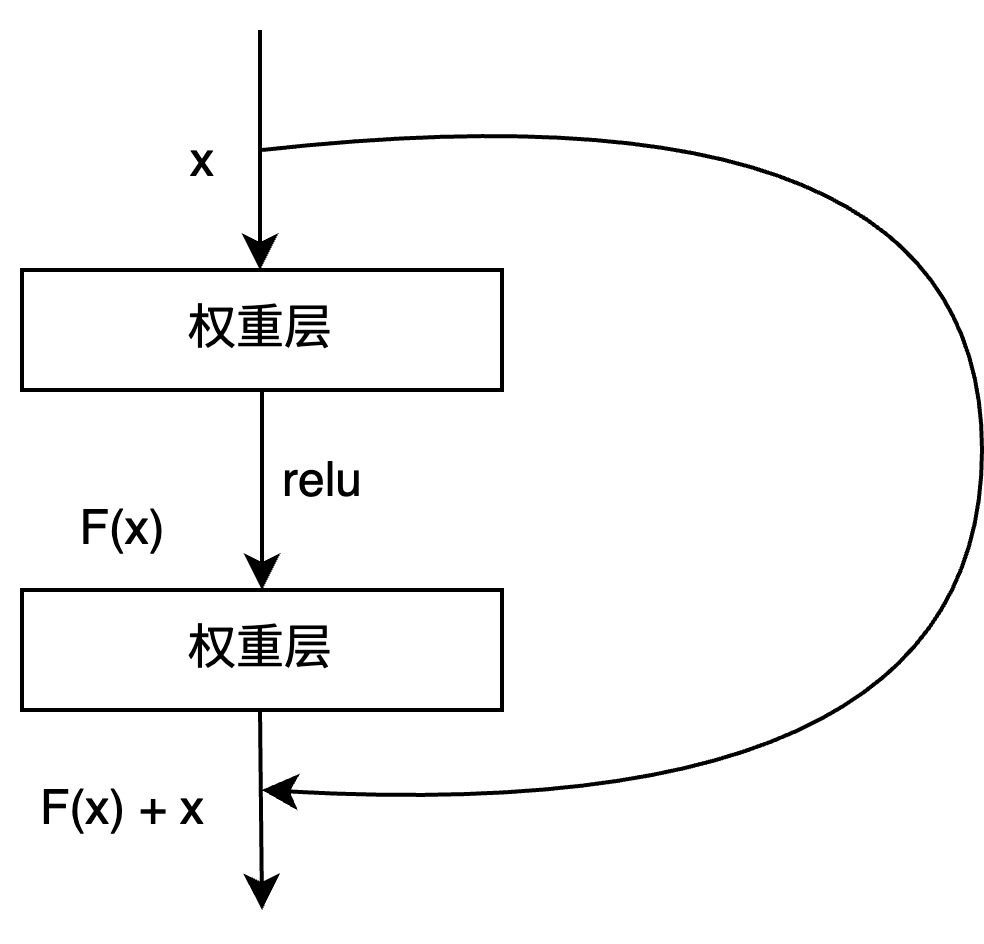
\includegraphics[width=0.5\textwidth]{figures/residual_block.png}
  \caption{残差模块}
  \label{residual_block}
\end{figure}

通常情况下让某一层网络学习恒等映射函数 $H(x) = x$ 比较困难,但是如果把网络函数设置为 $H(x) = F(x) + x$就可以吧恒等映射函数转化为一个残差函数 $F(x) = H(x) - x$,只要 $F(x) = 0$,就构成了一个恒等映射 $H(x) = x$。图\ref{residual_block}中,
iden mapping 被称为 shortcut 连接,residual mapping 即是 F(x)。残差的网络思想,如果网络已经到达最优,继续加深网络,residual mapping 将被 push 为 0,只剩下 identity mapping,这样理论上网络一直处于最优状态了,网络的性能也就不会随着深度增加而降低了。

实验证明,残差模块往往需要两层以上,单单一层的残差模块 并不能起到提升作用\cite{he2016deep}。shortcut 连接有两种,如果是同等维度的映射则 $F(x)=W_2σ(W_1x+b_1)+b_2,H(x)=F(x)+x$,
如果维度不同则 $F(x)=W_2σ(W_1x+b_1)+b_2,H(x)=F(x)+W_sx$。虽然残差模块刚开始是基于全连接层的表示,实际上残差模块可以用于卷积层。加法变为 channel 间的两个 feature map 逐个元素相加。下图\ref{residual_tcn}是时间卷积网络的残差模块。

\begin{figure}[htbp]
  \centering
  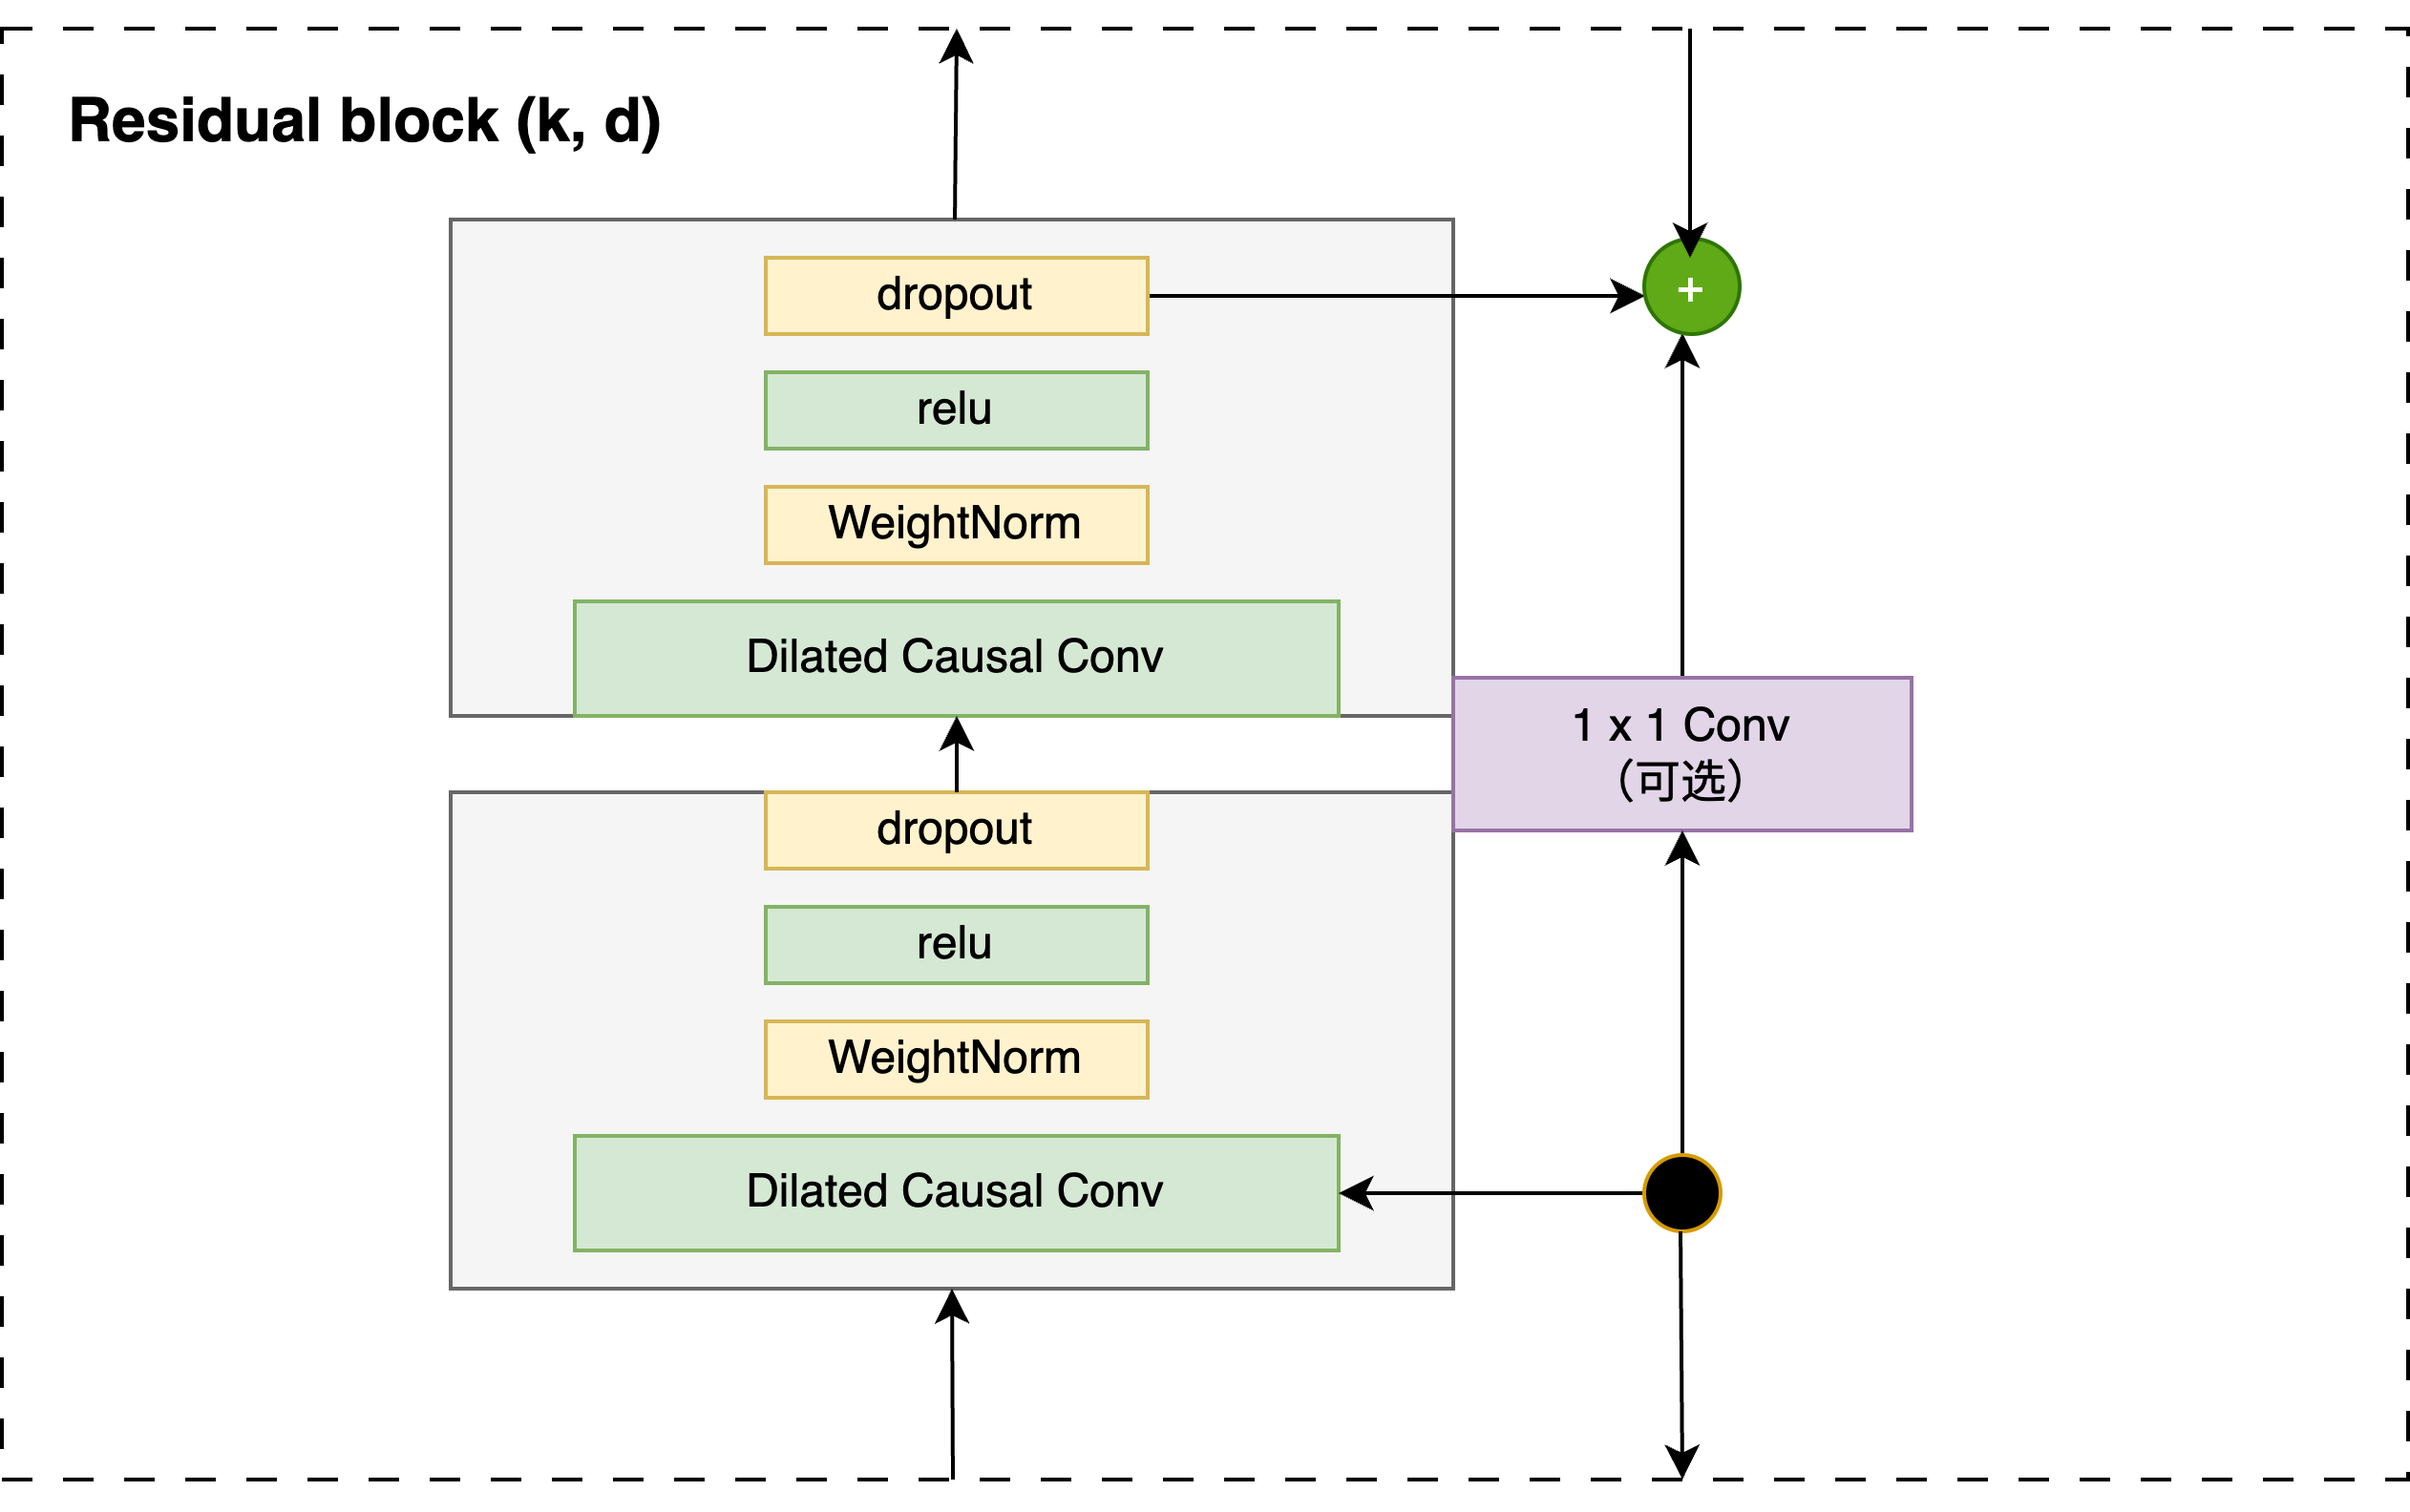
\includegraphics[width=\textwidth]{figures/resiual_tcn.png}
  \caption{TCN 的残差模块设计}
  \label{residual_tcn}
\end{figure}

于是整体的思路已经清晰,首先对时序数据集进行嵌入,嵌入使用指定大小的卷积核设置指定的膨胀因数,开始进行训练,进行归一向量化,和 ReLU 激活函数 Dropout 池化来防止梯度爆炸,最后用一个 Resnet 残差连接来避免梯度消失。

\section{时间卷积网络与负载情况的结合}
得到了综合负载评价指标和对应的时间就形成了一个常规的时间序列数据集,通过时间卷积网络深度学习即可较好的学习到时间序列内蕴藏的信息,通过蕴藏的信息预测未来的综合负载情况,返回给Nginx 集群内的负载均衡器,其以此来分配不同的不同的任务给空闲的服务器。

综合相关文献,对比了常规 RNN、LSTM、GRU 与 TCN 等循环神经网络在多种典型序列模型预测问题的性能表现上,结果表明 TCN 通常可以获得更好的预测精度,可以作为时间序列预测建模的有效手段\cite{bai2018empirical}\cite{赵洋2022基于时间卷积网络的短期电力负荷预测}。

(1)准备数据
通过使用监控脚本,周期性的收集 CPU、内存、磁盘 I/O 和网络带宽的利用率,并把这些数据保存到一个 CSV 文件中。由于作者本身的技能问题,不能使用高效率的监控程序,使用了 bash脚本来监控这些参数。

\begin{lstlisting}
#!/bin/bash

# 设置本地 CSV 文件路径
OUTPUT_FILE="/path/to/your/output_file.csv"

# 写入 CSV 文件的标题行
echo "Timestamp,CPU_Usage,Mem_Usage,Disk_Read,Disk_Write,Network_In,Network_Out" > $OUTPUT_FILE

# 设置网络接口名称
NETWORK_INTERFACE="eth0"

# 捕获信号,以便优雅地退出
trap "echo 'Script terminated'; exit" SIGHUP SIGINT SIGTERM

# 开始收集数据
while true; do
    # 获取 CPU 使用率
    CPU_USAGE=$(top -bn1 | grep "Cpu(s)" | awk '{print $2 + $4}')

    # 获取内存使用率 (使用的内存比例)
    MEM_USAGE=$(free -m | awk 'NR==2{printf "%.2f", $3*100/$2 }')

    # 获取磁盘读写数据 (需要 sysstat 包安装)
    DISK_IO=$(iostat -dx | awk 'NR>3 {print $6,$7}' | awk '{read+=$1; write+=$2} END {print read,write}')

    # 获取网络带宽使用数据 (需要 ifstat 包安装)
    NETWORK=$(ifstat -i $NETWORK_INTERFACE 1 1 | awk 'NR==3 {print $6,$8}')

    # 获取当前时间戳
    TIMESTAMP=$(date '+%Y-%m-%d %H:%M:%S')

    # 写入数据到 CSV
    echo "$TIMESTAMP,$CPU_USAGE,$MEM_USAGE,$DISK_IO,$NETWORK" >> $OUTPUT_FILE

    # 设置延迟时间,例如每隔 1 分钟收集一次数据
    sleep 60
done
\end{lstlisting}

这个脚本会无限循环到直到我手动暂停,可以设置循环次数,也可以设置循环大周期,比如使用 nohup 来进行循环次数的限制,使用每日,每周,每月作为一个大周期获得较为长远的数据,来进行更加准确的预测。通过主成分空间分析得到的原始数据集,然后分为按照 $9:1$ 分为训练集和测试集。

(2)TCN 参数设置

由膨胀因果卷积的原理可知,TCN 模型中的扩大因子$d$ 和卷积核大小 $K$ 是决定TCN 模型预测性能的主要参数。
此参数的选择目前尚无理论指导, 一般均需通过实验对比取得\cite{hewage2020temporal}。
由于实验数据以及实验环境的限制,无法通过实验来确定当前不同配置的TCN模型的 $MAE$ 值和 $RMSE$ 值来确定最佳参数。
但是可以列举几个比较通用的模型参数,其中, 扩大因子 d 分别取值为 2、4 、8 和 16 ;卷积核 K 分别取为 1×3、1×5 和 1×7 ,两组参数共构成 12 种组合形式,如下表所示。

% \usepackage{tabularray}
\begin{longtblr}[
  caption = {TCN 模型参数组合},
]{
  width = \linewidth,
  colspec = {Q[177]Q[158]Q[165]Q[183]Q[158]Q[160]},
  vline{4} = {-}{},
  vline{4} = {2}{-}{},
  hline{1,8} = {-}{0.08em},
}
序号 & $d$ & $K$ & 序号 & $d$ & $K$ \\
1  & 2     & 1x3   & 7  & 8     & 1x3   \\
2  & 2     & 1x5   & 8  & 8     & 1x5   \\
3  & 2     & 1x7   & 9  & 8     & 1x7   \\
4  & 4     & 1x3   & 10 & 16    & 1x3   \\
5  & 4     & 1x5   & 11 & 16    & 1x5   \\
6  & 4     & 1x7   & 12 & 16    & 1x7   
\end{longtblr}

通过使用不同参数的 TCN 模型可以得到 MAE(平均绝对误差)即观测值与预测值绝对差的平均值、RMSE(均方根误差)即观测值与预测值差的平方的平均值的平方根。来确定最佳参数。 通过指定训练参数 epoch 以及 lr 来获得预测值,在通过与观测值的比较即可选择到较好的模型参数。

(3)特征学习训练以及优化网络模型

指定时间卷积的参数扩大因子$d$ 和卷积核尺寸$K$,以及指定的 epoch 和 lr 开始训练;使用均方根误差作为目标函数计算预估值和真实值的误差,并利用 Adam 优化算法更新网络中的参数\cite{kingma2014adam}。下面是重要的训练代码。

\begin{lstlisting}
# 定义均方根误差为损失函数
class RMSELoss(nn.Module):
    def __init__(self):
        super().__init__()

    def forward(self, yhat, y):
        return torch.sqrt(torch.mean((yhat - y) ** 2))

# 初始化损失函数
loss_function = RMSELoss()
# 开始进行训练
for epoch in range(num_epochs):
    for batch in train_loader:
        inputs, targets = batch
        optimizer.zero_grad()  # 清除过往梯度
        outputs = model(inputs)  # 获取模型预测结果
        loss = loss_function(outputs, targets)  # 计算损失
        loss.backward()  # 反向传播,计算梯度
        optimizer.step()  # 使用 Adam 更新模型权重
\end{lstlisting}

(4)输出预估值

在PyTorch中,可以直接调用模型对象并直接将输入数据传递给它以获得预测值。
\begin{lstlisting}
# 切换模型到评估模式
model.eval()

# 不计算梯度来加速计算和减少内存消耗
with torch.no_grad():
    for inputs in test_loader:
        # 输入新数据集
        predictions = model(inputs)
        # 输出预测值
        print(predictions)
\end{lstlisting}

在上述的代码中,prediction变量包含了模型基于inputs给出的预测结果。如果是预测未来一个时间步,prediction可能只是一个数字。如果是预测未来多个时间步,prediction可能是一个Numpy数组或者PyTorch张量,其中包含一系列预测值。如果输入的一条数据,那么输出的就是单一的预测值,如果输入的是一个序列,那么输出的就是包含多个值的序列。可以通过预测后的序列值观察综合负载情况,然后进行判断。

\section{本章总结}

本章首先探讨了如何获取到剩余性能的数据,并根据科学的主成分分析法来选取合适的权重参数,用合适的权重参数得到了能较好体现负载情况的综合负载指标数据集。

接着讨论了时间卷积网络与其他循环神经网络的不同之处,得到了其在时间序列预测性能的特征和具体原理和具体过程。最后将综合负载指标已经对应的时间戳形成对应的时间序列数据集。通过设置 epoch 和 lr 来暂时确定 MAE 和 RMSE 的走势情况,以获取训练的最佳参数。
设置了最佳参数后可以进行更大的 epoch 来实现更好的预测性能。总体描述使用时间卷积网络来进行训练的步骤,分化训练集和测试集,然后根据上面得到的最佳参数设置,进行网络训练拟合,最后输出我们想要的预估值。


% 参考文献、致谢、附录等
\backmatter

% \bibliographystyle{gbt7714-unsrt.bst}%符合国标 GB/T 7714-2015 的文献风格
\bibliographystyle{zzubib.bst}%学校规范中示例文献风格
\bibliography{ref/refs}%参考文献

% 附录
% 研究生论文:综述
% \makeatletter
% \ifzzu@bachelor\else
%   %%================================================
%% Filename: review.tex
%% Encoding: UTF-8
%% Author: Yuan Xiaoshuai - yxshuai@gmail.com
%% Created: 2020-04-01 09:19
%% Last modified: 2020-04-05 20:38
%%================================================
\begin{review}

English words like `technology' stem from a Greek root beginning with
the letters $\tau\epsilon\chi\ldots\,$; and this same Greek word means {\sl
art\/} as well as technology. Hence the name \TeX, which is an
uppercase form of $\tau\epsilon\chi$. 

\section*{Section I}

Insiders pronounce the $\chi$ of \TeX\ as a Greek chi, not as an `x', so that
\TeX\ rhymes with the word blecchhh. It's the `ch' sound in Scottish words
like {\sl loch\/} or German words like {\sl ach\/}; it's a Spanish `j' and a
Russian `kh'. When you say it correctly to your computer, the terminal
may become slightly moist.

The purpose of this pronunciation exercise is to remind you that \TeX\ is
primarily concerned with high-quality technical manuscripts: Its emphasis is
on art and technology, as in the underlying Greek word. If you merely want
to produce a passably good document---something acceptable and basically
readable but not really beautiful---a simpler system will usually suffice.
With \TeX\ the goal is to produce the {\sl finest\/} quality; this requires
more attention to detail, but you will not find it much harder to go the
extra distance, and you'll be able to take special pride in the finished
product. 

\section*{Section II}

On the other hand, it's important to notice another thing about \TeX's name:
The `E' is out of kilter. This 
displaced `E' is a reminder that \TeX\ is about typesetting, and it
distinguishes \TeX\ from other system names. In fact, TEX (pronounced
{\sl tecks\/}) is the admirable {\sl Text EXecutive\/} processor developed by
Honeywell Information Systems. Since these two system names are
pronounced quite differently, they should also be spelled differently. The
correct way to refer to \TeX\ in a computer file, or when using some other
medium that doesn't allow lowering of the `E', is to type `TeX'. Then
there will be no confusion with similar names, and people will be
primed to pronounce everything properly.

\section*{References}

\begin{enumerate}[{$[$}1{$]$}]
\item Donald E. Knuth. The \TeX book. Addison-Wesley, 1984. ISBN: 0-201-13448-9
\item Paul W. Abrahams, Karl Berry and Kathryn A. Hargreaves. \TeX\ for the
  Impatient. Addison-Wesley, 1990. ISBN: 0-201-51375-7
\item David Salomon. The advanced \TeX book.  New York : Springer, 1995. ISBN:0-387-94556-3
\end{enumerate}

\end{review}
% \fi
% \makeatother

\makeatletter%致谢,研究生论文中在参考文献后,附录前
\ifzzu@bachelor\else
  %%================================================
%% Filename: ack.tex
%% Encoding: UTF-8
%% Author: Yuan Xiaoshuai - yxshuai@gmail.com
%% Created: 2012-01-12 18:09
%% Last modified: 2016-08-28 21:05
%%================================================
\begin{ack}
在毕业之际,以毕业论文的方式结束大学四年的美好时光。在撰写毕业论文的过程中,深刻体会到法学知识就像建房子,扎实的知识基础才会有牢固的地基,构建好论文的框架和清析的逻辑思维才能写好一篇有质量的论文。此次的毕业论文也让我知道,独立的思考善于发现问题是作为一名计算机人应具备的美好品质。

本次毕业论文能顺利完成首先最感谢的是我的指导老师张格老师,从我们论文的选题、开题报告、一稿、二稿、定稿和最终稿,张格老师都以最负责、最认真的态度给我们进行指导,对学生的毕业论文进行严格把关,针对我们的论文进行专业的指导,针对我们存在的问题,给予有建设性的建议,给学生进行论文修改带来了很多便利。对张格老师表示诚挚的感谢。其次也非常感谢对我予以帮助的同学,感谢你们在我写作的过程中,遇到困惑时给予我帮助,对于我的毕业论文完成也起到关键作用。

感谢科技的发展,如果没有日新月异的大模型,就不能做出很多相关的实验。感谢网友的网友的指导,没有你们就没有论文的方向,感谢论文的参考文献的作者们,你们提供给我的理论支持和实验数据,是我论文的骨干。感谢父母背后对我的资金的支持和精神上的支持,没有你就没有安稳地写作环境。

大学四年即将画上圆满的句号,在此也感谢各位任课老师大学四年的教导。对于论文老师指出存在的问题,我会虚心听取,积极的改进。在此再次向各位帮助过我的老师和同学们表示诚挚的感谢。

\begin{center}
    请君试问东流水,别意与之谁短长。

    山水有相逢,来日皆可期。
\end{center}

\end{ack}

\fi
\makeatother

% 附录
% 本科生论文三个附录,分别是附表,外文翻译和外文原文
% 研究生论文无具体要求
\makeatletter
\ifzzu@bachelor
  \begin{appendix}
    %%================================================
%% Filename: app01.tex
%% Encoding: UTF-8
%% Author: Yuan Xiaoshuai - yxshuai@gmail.com
%% Created: 2012-04-25 15:16
%% Last modified: 2019-11-07 12:55
%%================================================
\chapter{表格附件}
% 替换相应表格即可

\section*{毕业设计(论文)任务书}
\addcontentsline{toc}{section}{附表~1:毕业设计(论文)任务书}

\clearpage
\section*{郑州大学毕业论文开题报告表}
\addcontentsline{toc}{section}{附表~2:郑州大学毕业论文开题报告表}

\clearpage
\section*{毕业设计(论文)计划进程表}
\addcontentsline{toc}{section}{附表~3:毕业设计(论文)计划进程表}

\clearpage
\section*{郑州大学毕业设计中期检查表}
\addcontentsline{toc}{section}{附表~4:郑州大学毕业设计中期检查表}

\clearpage
\section*{毕业设计(论文)成绩评定表}
\addcontentsline{toc}{section}{附表~5:毕业设计(论文)成绩评定表}
    %%================================================
%% Filename: app02.tex
%% Encoding: UTF-8
%% Author: Yuan Xiaoshuai - yxshuai@gmail.com
%% Created: 2012-05-04 18:51
%% Last modified: 2016-08-28 21:06
%%================================================
\chapter{\sl The Name of the Game}

English words like `technology' stem from a Greek root beginning with
the letters $\tau\epsilon\chi\ldots\,$; and this same Greek word means {\sl
art\/} as well as technology. Hence the name \TeX, which is an
uppercase form of $\tau\epsilon\chi$.

Insiders pronounce the $\chi$ of \TeX\ as a Greek chi, not as an `x', so that
\TeX\ rhymes with the word blecchhh. It's the `ch' sound in Scottish words
like {\sl loch\/} or German words like {\sl ach\/}; it's a Spanish `j' and a
Russian `kh'. When you say it correctly to your computer, the terminal
may become slightly moist.

The purpose of this pronunciation exercise is to remind you that \TeX\ is
primarily concerned with high-quality technical manuscripts: Its emphasis is
on art and technology, as in the underlying Greek word. If you merely want
to produce a passably good document---something acceptable and basically
readable but not really beautiful---a simpler system will usually suffice.
With \TeX\ the goal is to produce the {\sl finest\/} quality; this requires
more attention to detail, but you will not find it much harder to go the
extra distance, and you'll be able to take special pride in the finished
product. 

On the other hand, it's important to notice another thing about \TeX's name:
The `E' is out of kilter. This 
displaced `E' is a reminder that \TeX\ is about typesetting, and it
distinguishes \TeX\ from other system names. In fact, TEX (pronounced
{\sl tecks\/}) is the admirable {\sl Text EXecutive\/} processor developed by
Honeywell Information Systems. Since these two system names are
pronounced quite differently, they should also be spelled differently. The
correct way to refer to \TeX\ in a computer file, or when using some other
medium that doesn't allow lowering of the `E', is to type `TeX'. Then
there will be no confusion with similar names, and people will be
primed to pronounce everything properly.

\section*{References}
\noindent{\itshape NOTE: these references are only for demonstration, they are
  not real citations in the original text.}

\begin{enumerate}[{$[$}1{$]$}]
\item Donald E. Knuth. The \TeX book. Addison-Wesley, 1984. ISBN: 0-201-13448-9
\item Paul W. Abrahams, Karl Berry and Kathryn A. Hargreaves. \TeX\ for the
  Impatient. Addison-Wesley, 1990. ISBN: 0-201-51375-7
\item David Salomon. The advanced \TeX book.  New York : Springer, 1995. ISBN:0-387-94556-3
\end{enumerate}

    %%================================================
%% Filename: app03.tex
%% Encoding: UTF-8
%% Author: Yuan Xiaoshuai - yxshuai@gmail.com
%% Created: 2012-05-04 18:51
%% Last modified: 2016-08-28 21:07
%%================================================
\chapter{此名有诗意}

英语单词“technology”来源于以字母$\tau\epsilon\chi$……开头的希腊词根;
并且这个希腊单词除了technology的意思外也有art的意思。因此,名称\TeX{}是
$\tau\epsilon\chi$的大写格式。

在发音时,\TeX{}的$\chi$发音与希腊的chi一样, 而不是“x”,所以\TeX{}与blecchhh押
韵。“ch”听起来象苏格兰单词中的loch或者德语单词中的ach;它在西班牙语中是“j”,
在俄语中是“kh”。当你对着计算机正确读出时,终端屏幕上可能有点雾。

这个发音练习是提醒你,\TeX{}主要处理的是高质量的专业书稿:它的重点在艺术和专
业方面, 就象希腊单词的含义一样。如果你仅仅想得到一个过得去——可读下去但不那么
漂亮——的文书,那么简单的系统一般就够用了。使用\TeX{}的目的是得到最好的质量;
这就要在细节上花功夫,但是你不会认为它难到哪里去, 并且你会为所完成的作品感到
特别骄傲。

另一方面重要的是要注意到与\TeX{}名称有关的另一件事:“E”是错位的。这个偏移“E”
的标识提醒人们,\TeX{}与排版有关,并且把\TeX{}从其它系统的名称区别开来。实际
上,TEX(读音为tecks)是Honeywell Information Systems 的极好的Text EXecutive处
理器。因为这两个系统的名称读音差别很大,所以它们的拼写也不同。在计算机中表明
\TeX{}文件的正确方法,或者当所用的方式无法降低“E”时,就要写作“TeX”。这样,就
与类似的名称不会产生混淆,并且为人们可以x正确发音提供了条件。

  \end{appendix}
\fi
\makeatother

\makeatletter%个人简历
\ifzzu@bachelor\else
  %%================================================
%% Filename: resume.tex
%% Encoding: UTF-8
%% Author: Yuan Xiaoshuai - yxshuai@gmail.com
%% Created: 2012-01-12 18:07
%% Last modified: 2016-08-28 21:09
%%================================================
\begin{resume}

  \resumeitem{个人简历}

  xxxx 年 xx 月 xx 日出生于 xx 省 xx 县。
  
  xxxx 年 9 月考入 xx 大学 xx 系 xx 专业,xxxx 年 7 月本科毕业并获得 xx 学士学位。
  
  xxxx 年 9 月免试进入 xx 大学 xx 系攻读 xx 学位至今。

  \resumeitem{发表的学术论文} % 发表的和录用的合在一起

  \begin{enumerate}[{[}1{]}]
  \item Yang Y, Ren T L, Zhang L T, et al. Miniature microphone with silicon-
    based ferroelectric thin films. Integrated Ferroelectrics, 2003,
    52:229-235. (SCI 收录, 检索号:758FZ.)
  \item 杨轶, 张宁欣, 任天令, 等. 硅基铁电微声学器件中薄膜残余应力的研究. 中国机
    械工程, 2005, 16(14):1289-1291. (EI 收录, 检索号:0534931 2907.)
  \item 杨轶, 张宁欣, 任天令, 等. 集成铁电器件中的关键工艺研究. 仪器仪表学报,
    2003, 24(S4):192-193. (EI 源刊.)
  \item Yang Y, Ren T L, Zhu Y P, et al. PMUTs for handwriting recognition. In
    press. (已被 Integrated Ferroelectrics 录用. SCI 源刊.)
  \item Wu X M, Yang Y, Cai J, et al. Measurements of ferroelectric MEMS
    microphones. Integrated Ferroelectrics, 2005, 69:417-429. (SCI 收录, 检索号
    :896KM.)
  \item 贾泽, 杨轶, 陈兢, 等. 用于压电和电容微麦克风的体硅腐蚀相关研究. 压电与声
    光, 2006, 28(1):117-119. (EI 收录, 检索号:06129773469.)
  \item 伍晓明, 杨轶, 张宁欣, 等. 基于MEMS技术的集成铁电硅微麦克风. 中国集成电路, 
    2003, 53:59-61.
  \end{enumerate}

  \resumeitem{研究成果} % 有就写,没有就删除
  \begin{enumerate}[{[}1{]}]
  \item 任天令, 杨轶, 朱一平, 等. 硅基铁电微声学传感器畴极化区域控制和电极连接的
    方法: 中国, CN1602118A. (中国专利公开号.)
  \item Ren T L, Yang Y, Zhu Y P, et al. Piezoelectric micro acoustic sensor
    based on ferroelectric materials: USA, No.11/215, 102. (美国发明专利申请号.)
  \end{enumerate}
\end{resume}
%本科论文无要求
\fi
\makeatother

\makeatletter%致谢,本科论文在最后
\ifzzu@bachelor
  %%================================================
%% Filename: ack.tex
%% Encoding: UTF-8
%% Author: Yuan Xiaoshuai - yxshuai@gmail.com
%% Created: 2012-01-12 18:09
%% Last modified: 2016-08-28 21:05
%%================================================
\begin{ack}
在毕业之际,以毕业论文的方式结束大学四年的美好时光。在撰写毕业论文的过程中,深刻体会到法学知识就像建房子,扎实的知识基础才会有牢固的地基,构建好论文的框架和清析的逻辑思维才能写好一篇有质量的论文。此次的毕业论文也让我知道,独立的思考善于发现问题是作为一名计算机人应具备的美好品质。

本次毕业论文能顺利完成首先最感谢的是我的指导老师张格老师,从我们论文的选题、开题报告、一稿、二稿、定稿和最终稿,张格老师都以最负责、最认真的态度给我们进行指导,对学生的毕业论文进行严格把关,针对我们的论文进行专业的指导,针对我们存在的问题,给予有建设性的建议,给学生进行论文修改带来了很多便利。对张格老师表示诚挚的感谢。其次也非常感谢对我予以帮助的同学,感谢你们在我写作的过程中,遇到困惑时给予我帮助,对于我的毕业论文完成也起到关键作用。

感谢科技的发展,如果没有日新月异的大模型,就不能做出很多相关的实验。感谢网友的网友的指导,没有你们就没有论文的方向,感谢论文的参考文献的作者们,你们提供给我的理论支持和实验数据,是我论文的骨干。感谢父母背后对我的资金的支持和精神上的支持,没有你就没有安稳地写作环境。

大学四年即将画上圆满的句号,在此也感谢各位任课老师大学四年的教导。对于论文老师指出存在的问题,我会虚心听取,积极的改进。在此再次向各位帮助过我的老师和同学们表示诚挚的感谢。

\begin{center}
    请君试问东流水,别意与之谁短长。

    山水有相逢,来日皆可期。
\end{center}

\end{ack}

\else\fi
\makeatother

\end{document}
